\documentclass[12pt]{article} %***
\usepackage[sectionbib]{natbib}
\usepackage{array,epsfig,fancyheadings,rotating}
\usepackage[]{hyperref}  %<----modified by Ivan
%%%%%%%%%%%%%%%%%%%%%%%%%%%%%%%%%%%%
\usepackage{sectsty, secdot}
%\sectionfont{\fontsize{12}{15}\selectfont}
\sectionfont{\fontsize{12}{14pt plus.8pt minus .6pt}\selectfont}
\renewcommand{\theequation}{\thesection\arabic{equation}}
\subsectionfont{\fontsize{12}{14pt plus.8pt minus .6pt}\selectfont}
%%%%%%%%%%%%%%%%%%%%%%%%%%%%%%%%%%%%%%%%%%%%%%%%%%%%%%%%%%%%%%%%%%%%%%%%%%%%%%%%%%%%%%%%

\textwidth=31.9pc
\textheight=46.5pc
\oddsidemargin=1pc
\evensidemargin=1pc
\headsep=15pt
%\headheight=.2cm
\topmargin=.6cm
\parindent=1.7pc
\parskip=0pt

\usepackage{amsmath}
\usepackage{amssymb}
\usepackage{amsfonts}
\usepackage{multirow}
\usepackage{amsthm}
\usepackage[title]{appendix}

\usepackage{bm}
\usepackage{graphicx}
\usepackage{color}
\usepackage{booktabs}
\usepackage{algorithm}
\usepackage{algorithmic}
\usepackage{IEEEtrantools}
\usepackage{enumerate}



\DeclareMathOperator{\mytr}{tr}
\DeclareMathOperator{\mydiag}{diag}
\DeclareMathOperator{\myrank}{Rank}
\DeclareMathOperator{\myE}{E}
\DeclareMathOperator{\myVar}{Var}
\DeclareMathOperator*{\argmax}{arg\,max}
\DeclareMathOperator*{\argmin}{arg\,min}

\newcommand{\bQ}{\mathbf{Q}}
\newcommand{\bZ}{\mathbf{Z}}
\newcommand{\bA}{\mathbf{A}}
\newcommand{\bB}{\mathbf{B}}
\newcommand{\bE}{\mathbf{E}}
\newcommand{\bF}{\mathbf{F}}
\newcommand{\bX}{\mathbf{X}}
\newcommand{\bP}{\mathbf{P}}
\newcommand{\bY}{\mathbf{Y}}
\newcommand{\bH}{\mathbf{H}}
\newcommand{\bG}{\mathbf{G}}
\newcommand{\bJ}{\mathbf{J}}
\newcommand{\bC}{\mathbf{C}}
\newcommand{\bO}{\mathbf{O}}
\newcommand{\bR}{\mathbf{R}}
\newcommand{\bI}{\mathbf{I}}
\newcommand{\bU}{\mathbf{U}}
\newcommand{\bD}{\mathbf{D}}
\newcommand{\bV}{\mathbf{V}}
\newcommand{\bW}{\mathbf{W}}
\newcommand{\bL}{\mathbf{L}}

\newcommand{\bu}{\mathbf{u}}
\newcommand{\bw}{\mathbf{w}}

\newcommand{\ud}{\mathbf{d}}

\newcommand{\bfsym}[1]{\ensuremath{\boldsymbol{#1}}}
\def\blambda {\bfsym {\lambda}} 
\def\bLambda {\bfsym {\Lambda}} 
\def\bSigma {\bfsym {\Sigma}} 
\def\bTheta {\bfsym {\Theta}} 





\newtheorem{assumption}{Assumption}

\setcounter{page}{1}
\newtheorem{theorem}{Theorem}
\newtheorem{lemma}{Lemma}
\newtheorem{corollary}{Corollary}
\newtheorem{proposition}{Proposition}
\theoremstyle{definition}
\newtheorem{definition}{Definition}
%\newtheorem{proof}{Proof}
\newtheorem{example}{Example}
\newtheorem{remark}{Remark}
\pagestyle{fancy}

%%%%%%%%%%%%%%%%%%%%%%%%%%%%%%%%%%%%%%%%%%%%%%%%%%%%%%%%%%%%%%%%%%%%%%%%%%%%%%%%%%%%%%%%%%%%%%%%%%%%%%%%%%%%%%%%%%%%%%%%%%%%
\pagestyle{fancy}
\def\n{\noindent}
\lhead[\fancyplain{} \leftmark]{}
\chead[]{}
\rhead[]{\fancyplain{}\rightmark}
\cfoot{}
%\headrulewidth=0pt  %<-modified by Ivan

%%%%%%%%%%%%%%%%%%%%%%%%%%%%%%%%%%%%%%%%%%%%%%%%%%%%%%%%%%%%%%%%%%%%%%%%%%%%%%%%%%%%%%%%%%%%%%%%%%%%%%%%%%%%%%%%%%%%%%%%%%%%
%%%%%%%%%%%%%%%%%%%%%%%%%%%%%%%%%%%%%%%%%%%%%%%%%%%%%%%%%%%%%%%%%%%%%%%%%%%%%%%%%%%%%%%%%%%%%%%%%%%%%%%%%%%%%%%%%%%%%%%%%%%%

\begin{document}

%%%%%%%%%%%%%%%%%%%%%%%%%%%%%%%%%%%%%%%%%%%%%%%%%%%%%%%%%%%%%%%%%%%%%%%%%%%%%%%%%%%%%%%%%%%%%%%%%%%%%%%%%%%%%%%%%%%%%%%%%%%%
%%%%%%%%%%%%%%%%%%%%%%%%%%%%%%%%%%%%%%%%%%%%%%%%%%%%%%%%%%%%%%%%%%%%%%%%%%%%%%%%%%%%%%%%%%%%%%%%%%%%%%%%%%%%%%%%%%%%%%%%%%%%

\renewcommand{\baselinestretch}{2}

\markright{ \hbox{\footnotesize\rm Statistica Sinica
%{\footnotesize\bf 24} (201?), 000-000
}\hfill\\[-13pt]
\hbox{\footnotesize\rm
%\href{http://dx.doi.org/10.5705/ss.20??.???}{doi:http://dx.doi.org/10.5705/ss.20??.???}
}\hfill }

\markboth{\hfill{\footnotesize\rm Rui Wang AND Xingzhong Xu} \hfill}
{\hfill {\footnotesize\rm LEAST FAVORABLE DIRECTION TEST} \hfill}

\renewcommand{\thefootnote}{}
$\ $\par

%%%%%%%%%%%%%%%%%%%%%%%%%%%%%%%%%%%%%%%%%%%%%%%%%%%%%%%%%%%%%%%%%%%%%%%%%%%%%%%%%%%%%%%%%%%%%%%%%%%%%%%%%%%%%%%%%%%%%%%%%%%%

\fontsize{12}{14pt plus.8pt minus .6pt}\selectfont \vspace{0.8pc}
\centerline{\large\bf LEAST FAVORABLE DIRECTION TEST FOR }
\vspace{2pt} \centerline{\large\bf MULTIVARIATE ANALYSIS OF VARIANCE}
\vspace{2pt} \centerline{\large\bf IN HIGH DIMENSION}
\vspace{.4cm} \centerline{
    Rui Wang, Xingzhong Xu
} \vspace{.4cm} \centerline{\it
Beijing Institute of Technology
}
 \vspace{.55cm} \fontsize{9}{11.5pt plus.8pt minus
.6pt}\selectfont

%%%%%%%%%%%%%%%%%%%%%%%%%%%%%%%%%%%%%%%%%%%%%%%%%%%%%%%%%%%%%%%%%%%%%%%%%%%%%%%%%%%%%%%%%%%%%%%%%%%%%%%%%%%%%%%%%%%%%%%%%%%%

\begin{quotation}
\noindent {\it Abstract:}
This paper considers the problem of multivariate analysis of variance for normal samples.
    When the sample dimension is larger than the sample size, the classical likelihood ratio test is not defined since the likelihood function is unbounded.
    Based on the unboundedness of the likelihood function, we propose a new test called least favorable direction test.
    The asymptotic null distribution of the test statistic is derived and the local asymptotic power function of the test is also given.
    %{\color{red}
    %These asymptotic results also hold under spiked covariance matrix which can characterize the strong correlations between variables.
%}
    The asymptotic power function and simulations show that the proposed test has particular high power when variables are strongly correlated.

\vspace{9pt}
    \noindent {\it Key words and phrases:}
    High dimensional data, least favorable direction test, multivariate analysis of variance, principal component analysis, spiked covariance.
%Balanced incomplete block design, Hadamard matrix, nearly balanced incomplete block design, orthogonal array.
\par
\end{quotation}\par



\def\thefigure{\arabic{figure}}
\def\thetable{\arabic{table}}

\renewcommand{\theequation}{\thesection.\arabic{equation}}


\fontsize{12}{14pt plus.8pt minus .6pt}\selectfont

\setcounter{section}{1} %***
\setcounter{equation}{0} %-1
\noindent {\bf 1. Introduction}

Suppose there are $k$ ($k\geq 2$) independent samples of $p$-dimensional data.
Within the $i$th sample ($1\leq i\leq k$), the observations $\{X_{ij}\}_{j=1}^{n_i}$ are independent and identically distributed (iid) as $\mathcal{N}_p(\xi_i,\bSigma)$, the $p$-dimensional normal distribution with mean vector $\xi_i$ and common variance matrix $\bSigma$.
%Suppose there are $k$ normal populations with possibly different means $\xi_1,\ldots,\xi_k$, but all with the same variance $\bSigma$.
%Suppose we observe $k$ independent random samples, each from the distribution $\mathcal{N}_p(\xi_i,\bSigma)$, where $1\leq i\leq k$, $k\geq 2$ is a fixed constant, $\xi_i$ and $\bSigma$ are unknown parameters.
%Denote by $X_{ij}\in \mathbb{R}^p$ the $j$th observation in group $i$, $j=1,\ldots,n_i$, $i=1,\ldots, k$,  where $n_i$ is the samples size of group $i$, $1\leq i \leq k$.
We would like to test the hypotheses
\begin{equation}\label{hypothesis}
    H_0: \xi_1=\xi_2=\cdots=\xi_k\quad \text{v.s.}\quad H_1: \text{$\xi_i\neq \xi_j$ for some $i\neq j$}.
\end{equation}
This testing problem is known as one-way multivariate analysis of variance (MANOVA) and has been well studied when $p$ is small compared with $n$, where $n=\sum_{i=1}^k n_i$ is the total sample size.

Let $\bH=\sum_{i=1}^k n_i (\bar{\bX}_i-\bar{\bX})(\bar{\bX}_i-\bar{\bX})^T$ be the sum-of-squares between groups and $\bG=\sum_{i=1}^k \sum_{j=1}^{n_i}(X_{ij}-\bar{\bX}_i)(X_{ij}-\bar{\bX}_i)^T$ be the sum-of-squares within groups, where $\bar{\bX}_i=n_i^{-1}\sum_{j=1}^{n_i}X_{ij}$ is the sample mean of group $i$ and $\bar{\bX}=n^{-1}\sum_{i=1}^k\sum_{j=1}^{n_i}X_{ij}$ is the pooled sample mean.
   There are four classical test statistics for hypothesis~\eqref{hypothesis}, which are all based on the eigenvalues of $\bH\bG^{-1}$. 

   %\begin{IEEEeqnarray*}{CC}
       %\text{Wilks' Lambda:} \qquad& |G+H|/|G|\\
       %%\text{Pillai trace:} \qquad& \mytr[H(G+H)^{-1}]\\
       %\text{Hotelling-Lawley trace:}\qquad & \mytr[HG^{-1}]\\
       %\text{Roy's maximum root:} \qquad& \lambda_{\max}(HG^{-1})
   %\end{IEEEeqnarray*}

       \begin{center}
       \begin{tabular}{|cc|}
           \hline
       {Wilks' Lambda:} & $|\bG+\bH|/|\bG|$\\
       {Pillai trace:} & $\mytr[\bH(\bG+\bH)^{-1}]$\\
       {Hotelling-Lawley trace:} & $\mytr[\bH \bG^{-1}]$\\
       {Roy's maximum root:} & $\lambda_{1}(\bH \bG^{-1})$\\
           \hline
           \end{tabular}
       \end{center}

%There are four classical tests for hypothesis~\eqref{hypothesis}: Wilks' Lambda (which is also the LRT), Hotelling-Lawley trace, Pillai Trace and Roy's maximum root.


In some modern scientific applications, people would like to test hypothesis~\eqref{hypothesis} in high dimensional setting, i.e., $p$ is greater than $n$.
See, for example,~\citet{Verstynen1209} and~\citet{Tsai2009}.
%However, when $p>n-k$, the LRT for hypothesis~\eqref{hypothesis} is not well defined.
However, when $p\geq n$, the four classical test statistics are not defined.
  Researchers have done extensive work to study the testing problem~\eqref{hypothesis} in high dimensional setting.
 So far, most tests are designed for two-sample case, i.e., $k=2$.
  See, for example,~\citet{Bai1996Efiect},~\cite{Srivastava2007Multivariate},~\citet{Chen2010A},~\citet{Tony2013} and \citet{Feng2014Two}.
  Recently, some tests have also been introduced for the case of genenral $k$.~\cite{Schott2007Some} modified Hotelling-Lawley trace and proposed the test statistic
  %$$
  %T_{SC}=\frac{1}{\sqrt{n-1}}\big(
  %\frac{1}{k-1}\mytr\big(\sum_{i=1}^k n_i\bar{X}_i\bar{X}_i^T-n\bar{X}\bar{X}^T\big)-\frac{1}{n-k}\mytr\big(\sum_{i=1}^k \sum_{j=1}^{n_i}X_{ij}X_{ij}^T-\sum_{i=1}^k n_i\bar{X}_i\bar{X}_i^T\big)
  %\big),
  %$$
  %where $\bar{\bX}_i=n_i^{-1}\sum_{j=1}^{n_i}X_{ij}$ and $\bar{\bX}=n^{-1}\sum_{i=1}^k\sum_{j=1}^{n_i}X_{ij}$.
  $$
  T_{SC}=\frac{1}{\sqrt{n-1}}\Big(
  \frac{1}{k-1}\mytr\big(\bH\big)-\frac{1}{n-k}\mytr\big(\bG\big)
  \Big).
  $$
Statistic $T_{SC}$ is a representative of the so-called sum-of-squares type statistics as it is based on an estimation of squared Euclidean norm $\sum_{i=1}^k n_i\|\xi_i-\bar{\xi}\|^2$, where $\bar{\xi}=n^{-1}\sum_{i=1}^k n_i \xi_i$.
See~\cite{Srivastava2013},~\cite{Yamada2015} and~\cite{Chang2017} for some other sum-of-squares type test statistics.
In another work,~\cite{Cai2014High} proposed a test statistic 
  $$
  T_{CX}=\max_{1\leq i\leq p} \sum_{1\leq j<l\leq k}\frac{n_j n_l}{n_j+n_l}\frac{(\Omega(\bar{\bX}_j-\bar{\bX}_l))_i^2}{\omega_{ii}},
  $$
  where $\Omega=(\omega)_{ij}=\bSigma^{-1}$ is the precision matrix. When $\Omega$ is unknown, it is substituted by an estimator.
  Unlike $T_{SC}$, $T_{CX}$ is an extreme value type statistic.
  %Statistics $T_{CX}$ and $T_{SC}$ are the representatives of two popular methodologies for high dimensional tests.
  
  %Suppose $\{X_{i1},\ldots, X_{in_i}\}$ are iid\ distributed as $\mathcal{N}(\xi_i,\bSigma)$ for $1\leq i\leq K$.
%The $k$ samples are independent.
%%$\xi_i$, $i=1\ldots, k$ and $\bSigma>0$ are unknown. An interesting problem in multivariate analysis is to test the hypotheses
%\begin{equation}
    %H: \xi_1=\xi_2=\cdots=\xi_k\quad v.s.\quad K: \textrm{$\xi_i\neq \xi_j$ for some $i\neq j$}.
%\end{equation}
%The likelihood ratio test (LRT) has a dominated position in classical multivariate analysis.
   The likelihood ratio test (LRT) method has been very successful in leading to satisfactory procedures in many specific problems.
    However, the LRT statistic for hypotheses~\eqref{hypothesis}, i.e. Wilks' Lambda statistic, is not defined for $p>n-k$.
   In high dimensional setting, both sum-of-squares type statistics and extreme value type statistics are not based on likelihood function.
    This motivates us to construct a likelihood-based test in high dimensional setting.
    %Note that Roy's maximum root, one of the four classic test statistics, is derived by Roy's union intersection principle.
    In a recent work,~\cite{Zhao2016A} proposed a generalized likelihood ratio test in the context of one-sample mean vector test.
    They used a least favorable argument to construct a generalized likelihood ratio test statistic.
    %They wrote the null hypothesis as the intersection of a class of component hypotheses.
    %For each component hypotheses, the likelihood ratio test is constructed.
    Their simulation results showed that their test has good power performance, especially when the variables are correlated.


    In this paper, we propose a generalized likelihood ratio test statistic for hypotheses~\eqref{hypothesis} called least favorable direction (LFD) test statistic.
    The asymptotic distributions of the test statistic are derived.
    %An important correlation pattern is that the variation of variables are mainly driven by a small number of common factors.
    These asymptotic distributions are valid when the eigenvalues of covariance matrix are bounded or the covariance matrix has $r$ significantly large eigenvalues.
    The latter covariance structure, known as spiked covariance model, can characterize the strong correlations between variables. See, for example,~\citet{Fan2008High},~\citet{Cai2012Sparse},~\citet{Shen2013Consistency} and~\citet{Ma2015A}.
    The asymptotic null distribution of the proposed test statistic involves some unknown parameters.
    We substitute the unknown parameters by their consistent estimators and formulate a test with asymptotically correct level.
    The asymptotic local power function of LFD test is also given.
 It will be seen that the asymptotic local power function of LFD test doesn't rely on the large eigenvalues of the covariance matrix.
For most existing tests, however, the asymptotic power decreases as the large eigenvalues of the covariance matrix increase.
    Thus, LFD test is particularly powerful when variables are strongly correlated.
    Further simulations show the good performance of LFD test.

    The rest of the paper is organized  as follows.
    In Section~\ref{methodology}, we propose LFD test and give
    the asymptotic distributions of LFD test.
     Section~\ref{numerical} complements our study with numerical simulations.
     In Section~\ref{concluding}, we give a short discussion.
     Finally, the proofs are gathered in the Appendix.
    %Higher criticism CX are special case of UIT.




%\setcounter{section}{2} %***
%\setcounter{equation}{0} %-1
%\noindent {\bf 2. The Second Section}

 
\section{Least favorable direction test}\label{methodology}
We introduce some notations.
 Define the $p\times n$ pooled sample matrix $\bX$ as
 $$\bX=(X_{11},X_{12},\ldots,X_{1n_1},X_{21},X_{22},\ldots,X_{2n_2},\ldots,X_{k1},X_{k2},\ldots,X_{kn_k}).$$
 The sum-of-squares within groups $\bG$ can be written as $\bG=\bX(\bI_n-\bJ\bJ^T)\bX^T$ where
 $$
 \bJ=\begin{pmatrix}
     \frac{1}{\sqrt{n_1}}\mathbf{1}_{n_1}&\mathbf{0} & \mathbf{0}\\
     \mathbf{0}&\frac{1}{\sqrt{n_2}} \mathbf{1}_{n_2}& \mathbf{0}\\
     \vdots &\vdots &\vdots \\
     \mathbf{0}&\mathbf{0}&\frac{1}{\sqrt{n_k}}\mathbf{1}_{n_k}
 \end{pmatrix}
 $$
 is an $n\times k$ matrix
 and $\mathbf{1}_{n_i}$ is an $n_i$-dimensional vector with all elements equal to $1$, $i=1,\ldots, k$.
 Construct an $n\times (n-k)$ matrix $\tilde{\bJ}$ as 
 $$
 \tilde{\bJ}=\begin{pmatrix}
     \tilde{\bJ}_1&\mathbf{0} & \mathbf{0}\\
     \mathbf{0}&\tilde{\bJ}_2& \mathbf{0}\\
     \vdots &\vdots &\vdots \\
     \mathbf{0}&\mathbf{0}&\tilde{\bJ}_k
 \end{pmatrix},
 $$
 where $\tilde{\bJ}_i$ is an $n_i\times (n_{i}-1)$ matrix defined as
 $$
\tilde{\bJ}_i=\begin{pmatrix}
    \frac{1}{\sqrt{2}}&\frac{1}{\sqrt{6}}&\cdots&\frac{1}{\sqrt{(n_i-2)(n_i-1)}}&\frac{1}{\sqrt{(n_i-1)n_i}}\\
    -\frac{1}{\sqrt{2}}&\frac{1}{\sqrt{6}}&\cdots&\frac{1}{\sqrt{(n_i-2)(n_i-1)}}&\frac{1}{\sqrt{(n_i-1)n_i}}\\
    0&-\frac{2}{\sqrt{6}}&\cdots&\vdots&\vdots\\
    \vdots&\vdots&\cdots&-\frac{n_i-2}{\sqrt{(n_i-2)(n_i-1)}}&\frac{1}{\sqrt{(n_i-1)n_i}}\\
    0&0&\cdots&0&-\frac{n_i-1}{\sqrt{(n_i-1)n_i}}\\
\end{pmatrix}.
 $$
The matrix $\tilde{\bJ}$ is a column orthogonal matrix  satisfying $\tilde{\bJ}^T\tilde{\bJ}=\bI_{n-k}$ and $\tilde{\bJ}\tilde{\bJ}^T =\bI_n-\bJ\bJ^T$.
Let $\bY=\bX\tilde{\bJ}$ be a $p\times (n-k)$ random matrix.
Then $\bG$ can be written as
$$\bG=
\bY \bY^T.
$$

The sum-of-squares between groups $\bH$ can be written as
$$
        \bH=\bX(\bJ\bJ^T-\frac{1}{n}\mathbf{1}_n\mathbf{1}_n^T)\bX^T
=\bX \bJ(\bI_k-\frac{1}{n}\bJ^T\mathbf{1}_n \mathbf{1}_n^T \bJ)\bJ^T \bX^T.
$$
By some matrix algebra, we have $\bI_k-\frac{1}{n}\bJ^T\mathbf{1}_n \mathbf{1}_n^T \bJ=\bC\bC^T$
where $\bC$ is a $k\times (k-1)$ matrix defined as $\bC=\bC_1\bC_2$, and
 $$
\bC_1=\begin{pmatrix}
    \sqrt{n_1}&\sqrt{n_1}&\cdots&\sqrt{n_1}&\sqrt{n_1}\\
    -\frac{n_1}{\sqrt{n_2}}&\sqrt{n_2}&\cdots&\sqrt{n_2}&\sqrt{n_2}\\
    0&-\frac{n_1+n_2}{\sqrt{n_3}}&\cdots&\vdots&\vdots\\
    \vdots&\vdots&\cdots&-\frac{\sum_{i=1}^{k-2}n_i}{\sqrt{n_{k-1}}}&\sqrt{n_{k-1}}\\
    0&0&\cdots&0&-\frac{\sum_{i=1}^{k-1}n_i}{\sqrt{n_k}}\\
\end{pmatrix},
 $$
 $$
\bC_2=\begin{pmatrix}
    \frac{n_1(n_1+n_2)}{n_2}&0&\cdots&0\\
    0&\frac{(\sum_{i=1}^2 n_i)(\sum_{i=1}^3 n_i)}{n_3}&\cdots&0\\
    \vdots&\vdots&\cdots&\vdots\\
    0&0&\cdots&\frac{(\sum_{i=1}^{k-1} n_i)(\sum_{i=1}^k n_i)}{n_{k}}\\
\end{pmatrix}^{-\frac{1}{2}}.
$$
Then $\bH$ can be written as
\begin{equation*}
    \begin{aligned}
        \bH=\bX \bJ\bC \bC^T \bJ^T \bX^T.
    \end{aligned}
\end{equation*}
 Define $\bTheta=(\sqrt{n_1}\xi_1,\ldots,\sqrt{n_k}\xi_k)$
 and the null hypothesis $H_0$ is equivalent to $\bTheta \bC=\bO_{p\times (k-1)}$, where $\bO_{p\times (k-1)}$ is a $p\times (k-1)$ matrix with all elements equal to $0$.
 Thus, the hypotheses in~\eqref{hypothesis} are equivalent to
 $$
 H_0:\bTheta \bC=\bO_{p\times (k-1)}\quad \text{v.s.}\quad H_1: \bTheta \bC\neq \bO_{p\times (k-1)}.
 $$

In low dimensional setting, the testing problem~\eqref{hypothesis} is well studied.
A classical test statistic is Roy's maximum root which is constructed by~\cite{Roy1953} using his well-known union intersection principle.
%The difficulty occurs when $p\geq n$, where the four classical test statistics can not be defined.
%To construct test statistic in high dimensional setting, a simple idea is to reduce the problem~\eqref{hypothesis} to a class of univariate problems.
        The key idea is to decompose data $\bX$ into a set of univariate data $\{\bX_{a}=a^T \bX:\, a\in \mathbb{R}^p, a^T a=1\}$.
        This induces a decomposition of the null hypothesis and the alternative hypothesis:
        $$
        H_0=\bigcap_{a\in\mathbb{R}^p, a^T a=1} H_{0a} \quad \text{v.s.} \quad 
        H_1=\bigcup_{a\in\mathbb{R}^p, a^T a=1} H_{1a},
        $$
        where 
 $H_{0a}: a^T \bTheta \bC = \bO_{1\times (k-1)}$ and  $H_{1a} : a^T \bTheta \bC \neq \bO_{1\times (k-1)}$.
Let $L_0(a)$ and $L_1(a)$ be the maximum likelihood of $\bX_a$ under $H_{0a}$ and $H_{1a}$, respectively.
For each $a$ satisfying $a^T a=1$, the component LRT statistic
$$ \frac{L_1(a)}{L_0(a)}=\Big(\frac{a^T(\bG+\bH) a}{a^T \bG a}\Big)^{n/2}$$
can be used to test $H_{0a}$ v.s. $H_{1a}$. 
Using union intersection principle, Roy proposed the test statistic
$
\max_{a^T a=1}  {L_1(a)}/{L_0(a)}=\lambda_{1}^{n/2}(\bH\bG^{-1}),
$
where $\lambda_{i}(\cdot)$ means the $i$th largest eigenvalue.
This statistic is an increasing function of Roy's maximum root.
%It turns out that many tests in the literature can be derived by the above strategy.
%While the LRT may be the best choice of univariate problems in step 2,
% there are more choices in step 1 and step 3.
%In step 3, Roy's union intersection principle suggests using $\max_{\gamma\in\Gamma}T_{\gamma}$ as a global test statistic~\citep{Roy1953},
%while another choice is to integrate $T_\gamma$ according to some measure $\mu(\gamma)$ and use $\int_\gamma T_{\gamma}\,\mu(d\gamma)$ as global test statistic.
%For step 1, we consider two different constructions of data projection.
%\begin{enumerate}[(i)]
%    \item
%        Consider the class of univariate data $\{\bX_{i}=e_i^T \bX:i=1,\ldots,p\}$, where $e_i$ is the $i$th standard basis in $\mathbb{R}^p$.
%        Hence $H_0=\bigcap_{i=1}^p H_{0i}$ and $H_1=\bigcup_{i=1}^p H_{1i}$, where
% $$
% H_{0i}: e_i^T \bTheta \bC = \bO_{1\times (k-1)}\quad \text{and}\quad H_{1a} : e_i^T \bTheta \bC \neq \bO_{1\times (k-1)}.
% $$
%\item
%    Consider the class of univariate data $\{\bX_{a}=a^T \bX:i=1,a\in\mathbb{R}^p, a^T a=1\}$.
%        Hence $H_0=\bigcap_{a\in \mathbb{R}^p, a^T a=1}H_{0a}$ and $H_1=\bigcup_{a\in \mathbb{R}^p,a^T a=1}H_{1a}$, where
% $$
% H_{0a}: a^T \bTheta \bC = \bO_{1\times (k-1)}\quad \text{and}\quad H_{1a} : a^T \bTheta \bC \neq \bO_{1\times (k-1)}.
% $$
%\end{enumerate}
%
%First, we consider the construction (i) in step 1.
%Suppose component test statistics 
%$$T_i={(k-1)^{-1}} e_i^T \bH e_i-(n-k)^{-1}e_i^T \bG e_i\quad i=1,\ldots, p$$
%are used in step 2, and in step 3 we integrate $T_i$ according to the uniform measure on $1,\ldots,p$. Then the resulting statistic is $p^{-1}\sum_{i=1}^p T_i$ which is equivalent to $T_{SC}$.
%If instead the likelihood ratio test statistic $e_i^T \bH e_i/e_i^T \bG e_i$ is used in step 2, one obtains a scalar invariant test statistic which is a direct generalization of~\citet{Srivastava2009A}'s test.
%On the other hand, by using data $\Omega^{-1}\bX$ and component test statistics
%$$
%T_i^*=\sum_{1\leq j<l \leq k} \frac{n_j n_l}{n_j+n_l}\frac{(\Omega(\bar{\bX}_j-\bar{\bX}_l))^2_i}{\omega_{ii}},
%$$
%we have $T_{CX}=\max_{1\leq i\leq p}T_i^*$.
%Here the component test statistic $T_i^*$ is similar to likelihood ratio tests.
%
%While many existing tests can be derived by the construction (i) in step 1, this construction has limitation in that it relies on the choice of an orthogonal basis of $\mathbb{R}^p$.
%In fact, test statistics resulting from this construction mostly requires certain prior information about the covariance matrix.
%For example,~\citet{Schott2007Some} requires that $\mytr(\bSigma^{2j})/p\to \tau_j\in(0,\infty)$, $j=1,2$, and~\citet{Cai2014High} requires a consistent estimator of $\Omega$.
%
%Next, we consider using construction (ii) in step 1, which does not rely on the basis of $\mathbb{R}^p$.
%Suppose the likelihood ratio test statistic $T_a=a^T \bH a/a^T \bG a$ is used in step 2.
%If we use the integrating strategy in step 3 and choose $\mu$ equal to the uniform distribution on the sphere, then the test statistic becomes
%$$
%\int_{a^T a=1} \frac{a^T \bH a}{a^T \bG a}\, \mu(da).
%$$
%Although it is hard to give an explicit form of the integration, we can approximate it by random projection.
%More specifically, one can randomly generate unit vectors $a_1,\ldots,a_M$ and the statistics can be approximated by $M^{-1}\sum_{i=1}^M a_i^T \bH a_i/a_i^T \bG a_i$.
%This statistic is well defined in high dimensional setting.
%A similar method is proposed by~\cite{Lopes2015A} for $k=2$ from a different point of view.
%Their analysis and simulations show that such random projection method has relatively good performance especially when variables are correlated.
%On the other hand, if $n-k\geq p$, Roy's union intersection principle can be used in step 3, the resulting  statistic is the well-known Roy's maximum root:
%$$
%\max_{a^T a=1}T_a=\lambda_{\max}(\bH \bG^{-1}).
%$$
%In fact, this statistic is first derived in~\cite{Roy1953} as an example of his union intersection principle.
%
%However, it can only be defined when $n-k\geq p$.
%In fact, if $p>n-k$, $G$ is not invertible and $T_a$ is not defined for some $a$. 
%We will follow~\citet{Zhao2016A}'s idea and propose a new test statistic for $p>n-k$.

From a likelihood point of view, log likelihood ratio is an estimator of the Kullback-Leibler divergence between the true distribution and the null distribution.
Hence the component LRT statistic $L_1(a)/L_0(a)$ characterizes the discrepancy between  the true distribution and the null distribution along the direction $a$.
%By maximizing $ (L_1(a)/L_0 (a))$, 
%one obtains component hypothesis $H_{0a^*}$, where $a^*=\argmax_{a^T a=1}(L_1(a)/L_0(a))$. 
This motivates us to consider the direction 
\begin{equation}\label{LFDdef1}
    a^*=\argmax_{a^T a=1}\frac{L_1(a)}{L_0(a)}
\end{equation}
which can hopefully achieve the largest discrepancy between the true distribution and the null distribution.
Thus, $H_{0a^*}$ is the component null hypothesis most likely to be not true.
We shall call $a^*$ the least favorable direction. %and $H_{0a^*}$ the least favorable hypothesis
Roy's maximum root is in fact the component LRT statistic along the least favorable direction.




%Note that $\max_{a^T a=1}\text{LRT}_a=\text{LRT}_{a^*}$, where 
%$a^*=\argmax_{a^T a=1}\text{LRT}_a$
%is the direction achieving the maximum discrepancy between the null hypothesis and alternative hypothesis.
%We shall call $a^*$ the rejection direction.
%In the derivation of Roy's maximum root, we have
%$$
%\text{LRT}_a=\Big(1+\frac{a^T H a}{a^T G a}\Big)^{n/2}.
%$$
%In another viewpoint, union intersection principle finds an direction $a$ along which the evidence against null hypothesis is maximized.
%Such an $a$ is data dependent.
%In the classical setting, the evidence of direction $a$ is $\text{LRT}_a$.
%In the current context, there are a class of $a$ such that $\text{LRT}_a$ achieve the infinity, the largest evidence in classical sense.
%We need to further choose a single $a$ from $\{a\,|\,\text{LRT}_a=+\infty\text{ and }a^T a =1\}$.
 %From the expression of $\text{LRT}_a$, we would like to make the largest discrepancy between $a^T H a$ and $a^T G a$.
%Note that if $\text{LRT}_{\alpha}=+\infty$, then $a^T G a=0$.
%Hence it's natural to choose $a$ as
%$$
        %a^{*}=
        %\argmax_{a^T a=1, a^T G a=0} 
        %a^T H a.
%$$
%Since $a^{*T}G a^*=0$, we propose the following test statistic for $H$:


Unfortunately, Roy's maximum root can only be defined when $n-k\geq p$, hence can not be used in the high dimensional setting.
%While it is hard to generalize Roy's maximum root to high dimensional setting, the least favorable hypothesis $a^*$ can be formally generalized to high dimensional setting.
In what follows, we assume $p>n-k$.
%The essence of Roy's union intersection principle is to find a direction $a$ along which $\text{LRT}_a$ is maximized.
%Based on this idea, we have the following heuristic argument to propose a new test statistic.
In this case,
the set
$$\mathcal{A}\overset{def}{=}\{a:L_1(a)=+\infty, \, a^T a=1\}=\{a:a^T \bG a=0, \, a^T a=1\}$$
is not empty since $\bG$ is singular. 
Consequently, the right hand side of~\eqref{LFDdef1} is not well defined since the ratio involves infinity.
Hence we need a new definition for LFD in the high dimensional setting.
Define
$$\mathcal{B}=\{a:L_0(a)=+\infty, \, a^T a=1\}=\{a:a^T (\bG+\bH)a= 0, \, a^T a=1\}.$$
It can be seen that $\mathcal{B}\subset \mathcal{A}$.
Moreover, by the independence of $\bG$ and $\bH$, with probability $1$, we have $\mathcal{A}\cap \mathcal{B}^c\neq \emptyset$.
Then for any direction $a$, there are three possible scenarios: $L_1(a)<+\infty$ and $L_0(a)<+\infty$; $L_1(a)=+\infty$ and $L_0(a)<+\infty$; $L_1(a)=+\infty$ and $L_0(a)=+\infty$.
To maximizes the discrepancy between $L_1(a)$ and $L_0(a)$, one may consider the direction $a$ such that $L_1(a)=+\infty$ and $L_0(a)<+\infty$.
This suggests that the least favorable direction $a^*$, which hopefully maximizes the discrepancy between $L_1(a)$ and $L_0(a)$, should be defined as $a^* = \argmin_{a\in\mathcal{A}\cap\mathcal{B}^c} L_0 (a)$.
%and take $H_{a^*}$ as the least favorable hypothesis.
Equivalently,
$$
\begin{aligned}
    a^*&=\argmin_{a\in \mathcal{A}\cap\mathcal{B}^c} L_0(a) = \argmax_{a^T a=1,a^T Ga=0} {a^T \bH a}.
\end{aligned}
$$
Based on $a^*$ and likelihood $L_0(a)$, we propose a new test statistic
\begin{equation*}
    \begin{aligned}
        T(\bX)=a^{*T} \bH a^*
        =
        \max_{a^T a=1, a^T \bG a=0} 
        a^T \bH a.
    \end{aligned}
\end{equation*}
We reject the null hypothesis when $T(\bX)$ is large enough.
We shall call $T(\bX)$ the LFD test statistic.
Since the least favorable direction $a^*$ is obtained from the component likelihood function, the statistic $T(\bX)$ is also a generalized likelihood ratio test statistic.
%The above method is first proposed by~\cite{Zhao2016A} in the context of testing one sample mean vector.
%The idea of generalized likelihood ratio test is first proposed by~\citet{Zhao2016A}.

Now we derive the explicit forms of LFD test statistic. 
%Let $J=\mathrm{diag}(n_1^{-1/2}\mathbf{1}_{n_1},\ldots,n_k^{-1/2}\mathbf{1}_{n_k})$.
%Then the matrices $I_n-JJ^T$, $JJ^T-\frac{1}{n}\mathbf{1}_n\mathbf{1}_n^T$ and $\frac{1}{n}\mathbf{1}_n\mathbf{1}_n^T$ are three $n\times n$ projection matrices which are pairwise orthogonal with rank $n-k$, $k-1$ and $1$.
%Let $\tilde{J}$ be a $n\times (n-k)$ matrix satisfying $\tilde{J}\tilde{J}^T =I-JJ^T$.
%Note that $I_k-\frac{1}{n}J^T\mathbf{1}_n \mathbf{1}_n^T J$ is a $k\times k$ projection matrix with rank $k-1$.
%Let $C$ be a $k\times (k-1)$ matrix satisfying $CC^T=I_k-\frac{1}{n}J^T\mathbf{1}_n \mathbf{1}_n^T J$.
%Then 
%$$
%G=Z(I_n-JJ^T)Z^T=
%Z\tilde{J}\tilde{J}^T Z^T.
%$$
%and
%\begin{equation*}
    %\begin{aligned}
        %F=\sum_{i=1}^k n_i (\bar{\mathbf{X}}_i-\bar{\mathbf{X}})(\bar{\mathbf{X}}_i-\bar{\mathbf{X}})^T 
        %=Z(JJ^T-\frac{1}{n}\mathbf{1}_n\mathbf{1}_n^T)Z^T
%=ZJ(I_k-\frac{1}{n}J^T\mathbf{1}_n \mathbf{1}_n^T J)J^T Z^T
%=ZJC C^T J^T Z^T.
    %\end{aligned}
%\end{equation*}
Let $\bY=\bU_{\bY}\bD_{\bY}\bV_{\bY}^T$ be the singular value decomposition of $\bY$, where $\bU_{\bY}$ and $\bV_{\bY}$ are $p\times (n-k)$ and $(n-k)\times(n-k)$ column orthogonal matrices, $\bD_{Y}$ is an $(n-k)\times (n-k)$ diagonal matrix.
Let $\bP_{\bY}=\bU_{\bY}\bU_{\bY}^T$ be the projection matrix on the column space of $\bY$.
Then Proposition~\ref{optProp} in Appendix implies that
\begin{equation}\label{statisticForm1}
\begin{aligned}
    T(\bX)
    %&=\lambda_{\max}\big(\bX \bJ\bC\bC^T\bJ^T\bX^T (\bI_p-
    %\bP_{\bY})
    %\big)
    =\lambda_{1}\big(\bC^T\bJ^T\bX^T (\bI_p-
    \bP_{\bY}
    )\bX\bJ\bC\big).
\end{aligned}
\end{equation}

%While~\eqref{statisticForm1} is convenient for theoretical analysis, it involves a projection matrix $\bP_{\bY}$ which is not easy to compute.
Next, we derive another simple form of $T(\bX)$.
%where $\bP_\bA=Z\tilde{J}{(\tilde{J}^T Z^T Z\tilde{J})}^{-1}\tilde{J}^T Z^T$.
By the relationship
\begin{equation*}
    \begin{aligned}
        \begin{pmatrix}
            \bJ^T \bX^T \bX\bJ & \bJ^T \bX^T \bX\tilde{\bJ}\\
            \tilde{\bJ}^T \bX^T \bX \bJ & \tilde{\bJ}^T \bX^T \bX \tilde{\bJ}
        \end{pmatrix}^{-1}
        =
        \Big(
        \begin{pmatrix}
            \bJ^T\\
            \tilde{\bJ}^T
        \end{pmatrix}
        \bX^T \bX
        \begin{pmatrix}
            \bJ &\tilde{\bJ}
        \end{pmatrix}
        \Big)^{-1}
        =
        \begin{pmatrix}
            \bJ^T {(\bX^T \bX)}^{-1}\bJ & \bJ^T {(\bX^T \bX)}^{-1}\tilde{\bJ}\\
            \tilde{\bJ}^T {(\bX^T \bX)}^{-1}\bJ & \tilde{\bJ}^T {(\bX^T \bX)}^{-1} \tilde{\bJ}
        \end{pmatrix}
    \end{aligned}
\end{equation*}
and matrix inverse formula, we have that
\begin{equation*}
    \begin{aligned}
        &{\big( \bJ^T {(\bX^T \bX)}^{-1}\bJ \big)}^{-1}
        =\bJ^T \bX^T \bX \bJ - \bJ^T \bX^T \bX\tilde{\bJ}{(\tilde{\bJ}^T \bX^T \bX \tilde{\bJ})}^{-1}
            \tilde{\bJ}^T \bX^T \bX\bJ 
        = \bJ^T \bX^T( \bI_p- \bP_{\bY}) \bX \bJ.
    \end{aligned}
\end{equation*}
Thus, 
\begin{equation}\label{statisticForm2}
    \begin{aligned}
        T(\bX)=
        \lambda_{\max}\Big(\bC^T\big( \bJ^T (\bX^T \bX)^{-1}\bJ \big)^{-1}\bC\Big).
    \end{aligned}
\end{equation}
Compared with~\eqref{statisticForm1},~\eqref{statisticForm2} doesn't involve $\bP_{\bY}$.
Hence~\eqref{statisticForm2} is convenient for computation.
In the case of $k=2$, the least favorable direction is propotional to
$
(\bI_p-\bP_{\bY}) (\bar{\bX}_1-\bar{\bX}_2)
$ and LFD test statistic has expression
$$
T(\bX)=\frac{n_1 n_2}{n_1+n_2}\| (\bI_p-\bP_{\bY}) (\bar{\bX}_1-\bar{\bX}_2)\|^2.
$$
In this case, 
the least favorable direction coincides with the maximal data piling direction proposed by~\cite{Ahn2010}.


Now we derive the asymptotic distribution of LFD test statistic.
We are especially interested in the case where variables are correlated.
For some real world problems, variables are heavily correlated with common factors, then the covariance matrix $\bSigma$ is spiked in the sense that a few eigenvalues of $\bSigma$ are significantly larger than the others~\citep{Fan2008High,Cai2012Sparse,Shen2013Consistency,Ma2015A}.
To characterize this correlation pattern, we make the following assumption for the eigenvalues of $\bSigma$.
%In this section, we investigate the asymptotic behavior of the new test statistic when $p$ is much larger than $n$.
%In high dimensional setting, it is a common phenomenon that the asymptotic distribution of a statistic relies on the covariance structure~\citep{Ma2015A}.
%We shall derive the asymptotic distribution of our statistic under two different covariance structures: non-spiked covariance and spiked covariance.




\begin{assumption}\label{assumpEigen}
    Let $\blambda_1\geq \blambda_2\geq \cdots \geq \blambda_p$ be the eigenvalues of $\bSigma$.
    Suppose there are $r\geq 0$ eigenvalues significantly larger than the others.
    We assume that
    \begin{itemize}
        \item
     $r=o(n)$.
\item
 $c_1 \geq \blambda_{r+1} \geq \ldots \geq \blambda_{p} \geq c_2$ for some positive absolute constants $c_1$ and $c_2$.
            \item
    If $r\neq 0$, we assume 
    $$\frac{\blambda_r n}{p}\to \infty,\quad
    \frac{\blambda_1^2 pr^2}{\blambda_r^2 n^2}\to 0\quad
        \frac{\log \blambda_r}{n}\to 0.$$
    \end{itemize}
\end{assumption}

\begin{remark}
    If $r=0$, Assumption~\ref{assumpEigen} becomes
    $
   c_1 \geq \blambda_{1} \geq \ldots \geq \blambda_{p} \geq c_2
    $.
    This is equivalent to Condition (C1) in~\cite{Cai2014High}.
    In fact, most existing high dimensional tests require conditions like this to avoid large eigenvalues.
    If $r>0$, the covariance matrix is spiked.
The spiked covariance model is commonly assumed in the study of PCA theory.
Many existing works in PCA study assume that $r$ is fixed.
    Here we allow $r$ to vary as a smaller order of $n$.
\end{remark}
%\begin{remark}
    %The condition $\blambda_r n/p\to \infty$ requires $\blambda_r$ to be much larger than $p/n$. This is satisfied, for example, for the factor model adopted by~\citet{Ma2015A}.
%\end{remark}
\begin{remark}
    If $r>0$, the harshest condition is $\blambda_1^2 p r^2 /(\blambda_r^2 n^2)\to 0$.
    If $\blambda_1$ and $\blambda_r$ are of the same order and $r$ is fixed, this condition is equivalent to $p/n^2\to 0$.
    We require this condition since the PCA consistency results are not valid when $p$ is too large. See, for example,~\citep{Cai2012Sparse}.
    This condition is unavoidable and the asymptotic behavior of $T(\bX)$ is different if this condition is violated.
\end{remark}


To establish the asymptotic distribution of $T(\bX)$ under Assumption~\ref{assumpEigen},
we need following notations.
Let $\bW_{k-1}$ be a $(k-1)\times(k-1)$ symmetric random matrix whose entries above the main diagonal are iid $\mathcal{N}(0,1)$ and the entries on the diagonal are iid $\mathcal{N}(0,2)$.
Let $\bSigma= \bU\bLambda \bU^T$ denote the eigenvalue decomposition of $\bSigma$, where $\bLambda =\mydiag (\blambda_1,\ldots,\blambda_p)$.
We denote $\bU=(\bU_1,\bU_2)$ where $\bU_1$ is $p\times r$ and $\bU_2$ is $p\times (p-r)$.
Denote $\bLambda_1=\mydiag(\blambda_1,\ldots,\blambda_r)$ and $\bLambda_2=\mydiag(\blambda_{r+1},\ldots,\blambda_p)$.
Then $\bSigma=\bU_1\bLambda_1 \bU_1^T+\bU_2\bLambda_2 \bU_2^T$.

The following theorem establishes the asymptotic distribution of LFD test statistic.
\begin{theorem}\label{thm1}
    Under Assumption~\ref{assumpEigen}, suppose $p/n\to \infty$ and
    $$
    \mytr\Big(\bLambda_2-\frac{1}{p-r}\mytr (\bLambda_2)\bI_{p-r}\Big)^2=o\big(\frac{p}{n}\big).
    $$
    Then under local alternative hypothesis
    \begin{equation*}
        \frac{1}{\sqrt{p}}\|\bTheta \bC\|_F^2=O(1),
    \end{equation*}
    we have
    $$
    \begin{aligned}
        \frac{T(\bX)-\frac{p-r-n+k}{p-r}\mytr(\bLambda_2)}{\sqrt{\mytr (\bLambda_2^2)}}
        \sim
        \lambda_{\max}\Big(\bW_{k-1}+\tfrac{1}{\sqrt{\mytr(\bLambda_2^2)}} \bC^T \bTheta^T (\bI_p-\bP_{\bY})\bTheta \bC\Big)
        +o_P(1),
    \end{aligned}
    $$
    where $\sim$ means having the same distribution.
\end{theorem}
To gain some insight into the asymptotic behavior of $T(\bX)$, suppose the null hypothesis holds and $k=2$, then Theorem~\ref{thm1} implies that
$$
\frac{T(\bX)-\frac{p-r-n+k}{p-r}\mytr(\bLambda_2)}{\sqrt{2\mytr (\bLambda_2^2)}}\xrightarrow{\mathcal{L}}\mathcal{N}(0,1).
$$
The asymptotic variance of $T(\bX)$ is ${2\mytr (\bLambda_2^2)}$.
If $r=0$, it equals to ${2\mytr (\bSigma^2)}$ which is also the asymptotic variance of~\citet{Bai1996Efiect} and~\citet{Chen2010A}'s statistics.
In comparison, if $r>0$, ${2\mytr (\bLambda_2^2)}$ tends to be smaller than $2\mytr(\bSigma^2)$.
In fact, if $\liminf_{n\to \infty} \blambda_1/p \in (0,+\infty]$, we have
$$
\liminf_{n\to \infty}\frac{2\mytr(\bSigma^2)}{2\mytr(\bLambda_2^2)}\in (1,+\infty].
$$
The reason for this is because the projection matrix $\bI_p-\bP_{\bY}$ appeared in expression~\eqref{statisticForm1} can remove large variance terms of $\bX\bJ \bC$.

To formulate a test procedure with asymptotically correct level, the unknown parameters $r$, $\mytr(\bLambda_2)$ and $\mytr(\bLambda_2^2)$ should be estimated.
We use the following statistic to estimate $r$:
    $$
    \begin{aligned}
    \hat{r}=
            \begin{cases}
                \argmax_{1\leq i\leq n-k-1} \frac{\lambda_i(\bY^T \bY)}{\lambda_{i+1}(\bY^T \bY)}\geq \gamma_n\quad& \text{if } \max_{1\leq i\leq n-k-1}\frac{\lambda_i(\bY^T \bY)}{\lambda_{i+1}(\bY^T \bY)}\geq \gamma_n\\
                0\quad&\text{otherwise}\\
            \end{cases}
    \end{aligned}
    $$
where $\gamma_n$ is a hyper parameter slowly tending to $+\infty$ as $n\to \infty$.
The following proposition establishes the consistency of $\hat{r}$.
\begin{proposition}\label{numberConsistency}
    Suppose $p/n\to \infty$, $r=o(n)$, $\blambda_r n/p\to \infty$ and $c_1\geq\blambda_{r+1}\geq \ldots \geq \blambda_p\geq c_2$. If $\gamma_n\to \infty$ and $\gamma_n = o(n\blambda_r/p)$, then
 $\Pr(\hat{r}=r)\to 1$.
\end{proposition}
\begin{remark}
    For the factor model adopted by~\cite{Ma2015A}, $\lambda_r$ is of order $p$. Hence we can take $\gamma_n=\sqrt{n}$.
\end{remark}
    We use the following statistic to estimate $\mytr(\bLambda_2)$:
    $$\widehat{\mytr(\bLambda_2)}=\frac{1}{n-k}\sum_{i=\hat{r}+1}^{n-k}\lambda_i(\bY^T \bY).$$
\begin{proposition}\label{traceProp1}
    Under the assumptions of Theorem~\ref{thm1}, suppose $\gamma_n\to \infty$ and $\gamma_n=o({n\blambda_r}/{p})$, then
    $$\widehat{\mytr(\bLambda_2)}=\mytr(\bLambda_2)+o_P(\sqrt{p}).$$
\end{proposition}



%    Under non-spiked covariance, an unbiased estimator of $\mytr(\bSigma^2)$ is
%    $$
%    \widehat{\mytr(\bSigma^2)}=\frac{2}{(n-k)(n-k-1)}\sum_{1\leq i<j\leq n-k}(Y_i^T Y_j)^2.
%    $$
%    \begin{proposition}\label{prop:nonSpiked}
%    As $n\to \infty$,
%    $$
%    \frac{\widehat{\mytr(\bSigma^2)}}{\mytr(\bSigma^2)}\xrightarrow{P} 1.
%    $$
%    \end{proposition}
   % \begin{proof}
   %     Since $\myE (Y_i^T Y_j)^2=\mytr(\bSigma^2)$, $i\leq j$, we have
   % $$
   %     \myE\big(\widehat{\mytr(\bSigma^2)}\big)=\mytr(\bSigma^2).
   %     $$
   %     To prove the proposition, we only need to show that 
   %     $$
   %     \myVar\big(\widehat{\mytr(\bSigma^2)}\big) =o(\mytr^2(\bSigma^2)).
   %     $$
   %      Note that
   %      $$
   %     \begin{aligned}
   %         &\myE\big(\widehat{\mytr(\bSigma^2)}\big)^2 =
   %         \frac{4}{(n-k)^2(n-k-1)^2}\Big(\sum_{1\leq i < j\leq n-k}(Y_i^T Y_j)^2\Big)^2\\
   %         =&
   %         \frac{4}{(n-k)^2(n-k-1)^2}\myE\Big( \sum_{i<j}(Y_i^T Y_j)^4+
   %         \sum_{i<j,k<l:\{i,j\}\{k,l\}=\emptyset}(Y_i^T Y_j)^2 (Y_k^T Y_l)^2\\
   %         &+2\sum_{i<j<k}\big((Y_i^T Y_j)^2(Y_i Y_k)^2+(Y_i^T Y_j)^2(Y_j Y_k)^2+(Y_i^T Y_k)^2(Y_j Y_k)^2\big) \Big)\\
   %         =&
   % \frac{4}{(n-k)^2(n-k-1)^2}\Big(
   %         \frac{(n-k)(n-k-1)}{2}\big(6\mytr(\bSigma^4)+3\mytr^2(\bSigma^2)\big)\\
   %         &+\frac{(n-k)(n-k-1)(n-k-2)(n-k-3)}{4}\mytr^2(\bSigma^2)\\
   %         &+(n-k)(n-k-1)(n-k-2)\big(2\mytr(\bSigma^4)
   %         +\mytr^2(\bSigma^2)\big)
   %         \Big)\\
   %         =&
   %         \mytr^2(\bSigma^2)(1+o(1)).
   %     \end{aligned}
   %      $$
   %      Then
   %     $$
   %     \myVar\big(\widehat{\mytr(\bSigma^2)}\big) =
   %         \myE\big(\widehat{\mytr(\bSigma^2)}\big)^2 - 
   %         \big(\myE\big(\widehat{\mytr(\bSigma^2)}\big)\big)^2=
   %         o(\mytr^2(\bSigma^2)).
   %     $$
   %     This completes the proof.
   % \end{proof}
    %Under the assumptions of Theorem~\ref{nonSpiked}.


 To estimate $\mytr(\bLambda_2^2)$,
    we use the idea of leave-two-out.
    Let $\bY_{(i,j)}$ be a $p\times (n-k-2)$ matrix obtained by deleting the $i$th and $j$th columns from $\bY$.
    Let $\bY_{(i,j)}=\bU_{\bY;{(i,j)}}\bD_{\bY;{(i,j)}}\bV_{\bY;{(i,j)}}^T$ denote the singular value decomposition of $\bY_{(i,j)}$.
    Here $\bU_{\bY;{(i,j)}}$ is a $p\times (n-k-2)$ column orthogonal matrix.
    Let $\tilde{\bU}_{\bY;{(i,j)}}$ be a $p\times (p-n+k+2)$ orthogonal matrix satisfying $\tilde{\bU}_{\bY;{(i,j)}}\tilde{\bU}_{\bY;{(i,j)}}^T=\bI_{p}-\bU_{\bY;{(i,j)}}\bU_{\bY;{(i,j)}}^T$.



    Let $w_{ij}$ be the $(i,j)$th element of $\bY^T \tilde{\bU}_{\bY;(i,j)} \tilde{\bU}_{\bY;(i,j)}^T \bY$.
    Define
    $$
    \widehat{\mytr(\bLambda_2^2)}=\frac{2}{(n-k)(n-k-1)}\sum_{1\leq i<j\leq n-k}w_{ij}^2.
    $$
    We use $\widehat{\mytr(\bLambda_2^2)}$ to estimate $\mytr(\bLambda_2^2)$.
    The following proposition shows that $\widehat{\mytr(\bLambda_2^2)}$ is  ratio consistent.
    \begin{proposition}\label{Taichangle}
        Under the assumptions of Theorem~\ref{thm1}, we have
        $$
        \frac{\widehat{\mytr(\bLambda^2_2)}}{\mytr(\bLambda^2_2)} \xrightarrow{P} 1.
        $$

    \end{proposition}


Now we can construct LFD test procedure with asymptotic correct level $\alpha$. Let 
$$
Q=\frac{T(\bX)-\frac{p-\hat{r}-n+k}{p-\hat{r}}\widehat{\mytr(\bLambda_2)}}{\sqrt{\widehat{\mytr(\bLambda_2^2)}}}.
$$
Let $F(x)$ be the cumulative distribution function of $\lambda_{1}(\bW_{k-1})$.
LFD test reject the null hypothesis if $Q> F^{-1}(1-\alpha)$.

Theorem~\ref{thm1}, Proposition~\ref{traceProp1} and Proposition~\ref{Taichangle} implies that the resulting test procedure has asymptotic correct level under the assumptions of Theorem~\ref{thm1}.
Moreover, by Theorem~\ref{thm1}, the asymptotic local power function of LFD test procedure is
$$
\Pr\Big(
        \lambda_{1}\big(\bW_{k-1}+\tfrac{1}{\sqrt{\mytr(\bLambda_2^2)}} \bC^T \bTheta^T (\bI_p-\bP_{\bY})\bTheta \bC\big)\geq F_{\bW}^{-1}(1-\alpha)
\Big).
$$
If $k=2$, the asymptotic local power function of~\cite{Bai1996Efiect} and~\cite{Chen2010A}'s method can be written as
$$
\Pr\Big(
        \lambda_{1}\big(\bW_{1}+\tfrac{1}{\sqrt{\mytr(\bSigma^2)}} \bC^T \bTheta^T \bTheta \bC\big)\geq F_{\bW}^{-1}(1-\alpha)
\Big).
$$
Hence the asymptotic relative efficiency between LFD test and~\cite{Bai1996Efiect} and~\cite{Chen2010A}'s method is
$$
 \sqrt{\frac{{{\mytr(\bSigma^2)}}}{{\mytr(\bLambda_2^2)}}}
\frac{ \bC^T \bTheta^T (\bI_p-\bP_{\bY})\bTheta \bC}{ {\bC^T \bTheta^T \bTheta \bC}}.
$$
There's a random term $\bP_{\bY}$ in the expression.
To overcome this,
suppose $\sqrt{n_i} \xi_i$ has prior distribution $\mathcal{N}_p(0,\psi \bI_p)$, $i=1,2$.
In this case,
$
\psi^{-1}\bC^T \bTheta^T \bTheta \bC$
is distributed as $\chi^2$ distribution with $p$ degrees of freedom.
%$ \text{Wishart}_{k-1}(p,\bI_{k-1})$, the $(k-1)$-dimensional Wishart distribution with degree of freedom $p$ and parameter $\bI_{k-1}$.
On the other hand,
$\bC^T \bTheta^T (\bI_p-\bP_{\bY})\bTheta \bC$  is distributed as 
%$\text{Wishart}_{k-1}(p-n+k,\bI_{k-1})$.
$\chi^2$ distribution with $p-n+k$ degrees of freedom.
In this case, we have
$$
\frac{\bC^T \bTheta^T (\bI_p-\bP_{\bY})\bTheta \bC}{\bC^T \bTheta^T \bTheta \bC}\xrightarrow{P}1.
$$
Thus, when
$$
\liminf_{n\to \infty}\frac{{{\mytr(\bSigma^2)}}}{{\mytr(\bLambda_2^2)}}\in(1,+\infty],
$$
LFD test tends to be more powerful than~\cite{Chen2010A}'s test.



%\section{Schott's method}

%$$
%E=ZZ^T-\sum_{i=1}^k n_i \bar{X}_i \bar{X}_i^T.
%$$

%$$
%H=\sum_{i=1}^{k} n_i \bar{X}_i \bar{X}_i^T - n\bar{X}\bar{X}^T.
%$$

%$$
%\mytr E = \mytr Z^T Z - \mytr J^T Z^T Z J.
%$$


%$$
%\mytr H = \mytr J^T Z^T Z J - \frac{1}{n} 1_n^T Z^T Z 1_n
%$$

%$$
%T_{SC}=\frac{1}{\sqrt{n-1}}(
%\frac{1}{k-1}\mytr H-\frac{1}{n-k} \mytr E
%)
%$$
%
%Our new test statistic comes from construction ii in step 1, the likelihood ratio test statistics in step 2 and strategy II in step 3.
%Theorems~\ref{nonSpiked} and~\ref{thm1} allow us to analyze the properties of the proposed test.
%Suppose $\sqrt{n_i}\mu_i$ is from prior distribution $\mathcal{N}_p(0,\psi \bI_p)$, $i=1,\ldots, k$.
%Then $\psi^{-1}\bC^T \bTheta^T \bTheta \bC$ is distributed as $\text{Wishart}_{k-1}(p,\bI_{k-1})$ (Wishart distribution with freedom $p$ and parameter $\bI_{k-1}$) and $\psi^{-1}\bC^T \bTheta^T \bP_{\bY}\bTheta \bC$ is distributed as $\text{Wishart}_{k-1}(n-k,\bI_{k-1})$.
%In this case, we have
%$$
%\psi^{-1}\bC^T \bTheta^T (\bI_P-\bP_{\bY})\bTheta \bC=
%(1+o_P(1))\psi^{-1}\bC^T \bTheta^T \bTheta \bC.
%$$
%If the conditions of Theorem~\ref{nonSpiked} hold and $k=2$, the asymptotic power of the proposed test is the same as that of~\cite{Bai1996Efiect}and~\cite{Chen2010A}'s method.
%Since the method of~\cite{Schott2007Some} is a direct generalization of~\cite{Bai1996Efiect}'s method, it can be shown the asymptotic power of the proposed test is the same as that of~\cite{Schott2007Some} for general $k$.
%Next, suppose the covariance matrix is spiked and the conditions of Theorem~\ref{thm1} hold.
%Theorem~\ref{thm1} implies that the proposed test does not depend on large eigenvalues $\lambda_1,\ldots,\lambda_r$ while other existing test procedures are negatively affected by large eigenvalues $\lambda_1,\ldots,\lambda_r$.   
%Thus, the new test has particular good power behavior when $\lambda_1,\ldots,\lambda_r$ are large.
% This property is not surprising since our statistic is from construction ii.
%As a result, our statistic has a wider applicable range compared with the tests from construction i.


%%%%%%%%%%%%%%%%% Hotelling-Lawley trace %%%%%%%%%%%%%%%%%%%%%%%%%
%Another classical test statistic, Hotelling-Lawley trace,  can also be derived by Roy's union intersection principle. This is shown by~\cite{Mudholkar1974}.
 %In that paper, they consider the transformed data $\{M^T \bX: M \textrm{ is } \text{$(k-1)\times p$ matrix}\}$ and the decomposition of hypotheses:
 %$$H_{0}=\bigcap_{M}H_{0M} \quad\text{and}\quad H_1=\bigcup_{M}H_{1M} ,$$
 %where
 %$$
 %H_{0M}: \mytr( M \bTheta C) = 0\quad \text{and}\quad H_{1M} : \mytr( M \bTheta C )> 0.
 %$$
%
%Note that $\myE Z=\bTheta J^T$, hence
%the uniformly minimum variance unbiased estimator of $\mytr(M\bTheta C)$ is $\mytr(MZJ C)$.
%It can be seen that
%$
%\mytr \big(MZJ C\big)
%\sim
%\mathcal{N}\big(\mytr(M\bTheta C),\mytr(M\bSigma M^T )\big)
%$.

%=====================
%$$
%\mytr \big(MZJC\big)
%=
%\mytr \big(CMZJ\big)
%$$
%$ZJ=(\sqrt{n_1}\bar{\bX}_1,\ldots,\sqrt{n_k}\bar{\bX}_k)$.
%Note that $CM\sqrt{n_i}\bar{\bX}_i\sim \mathcal{N}_{k-1}(\sqrt{n_i}CM\xi_i,CM\bSigma M^T C^T)$.
%Hence we have that
%$$
%\mytr \big(CMZJ\big)
%\sim
%\mathcal{N}(\mytr(CM\bTheta),\mytr(CM\bSigma M^T C^T))
%\sim
%\mathcal{N}(\mytr(M\bTheta C),\mytr(M\bSigma M^T )).
%$$
%==================

%Hence it's natural to use one side $t$ type statistic
%$$
%T_M = \frac{
%\mytr \big(MZJC\big)
%}{
    %\sqrt{\mytr(M G M^T)}
%}
%$$
%to test $H_M$ against $K_M$.



%By Cauchy inequality $\max_B \mytr(AB^T)/\mytr^{1/2}(BB^T)=\mytr^{1/2}(AA^T)$, we have
%$$
%\begin{aligned}
    %\max_M T_M &=\max_M \frac{\mytr \big(MG^{1/2}G^{-1/2}ZJC\big)
%}{\sqrt{\mytr(M G^{1/2} (M G^{1/2})^T)}
%}
    %=\mytr^{1/2}((ZJC)^T G^{-1}ZJC)\\
    %&=\mytr^{1/2}( ZJC(ZJC)^T G^{-1})
    %=\mytr^{1/2}(H G^{-1}).
%\end{aligned}
%$$

%====================
\section{Numerical study}\label{numerical}

In this section, we compare the numerical performance of LFD test with some existing tests, including the MANOVA tests of~\citet{Schott2007Some} and~\citet{Cai2014High} and the two sample tests of~\cite{Srivastava2007Multivariate},~\cite{Chen2010A},~\cite{Tony2013} and~\cite{Feng2014Two}.
 Note that the critical values of these existing tests are not valid under spiked covariance model.
Hence we use permutation method to determine the critical values throughout our simulations.
   The test procedures resulting from permutation method have exact levels as long as the null distribution of observations are exchangeable~\citep{Romano1990On}.
   The major down-side to permutation method is that it can be computationally intensive.
   Fortunately, for LFD test statistic,  the permutation method has a simple implementation.
    By expression~\eqref{statisticForm2}, a permuted statistic can be written as
    \begin{equation}\label{permutedStatistic}
        T(\bX\Gamma)=\lambda_{\max}\Big(\bC^T{\big( \bJ^T \Gamma^T {(\bX^T \bX)}^{-1} \Gamma \bJ \big)}^{-1}  \bC\Big),
    \end{equation}
where $\Gamma$ is an $n\times n$ permutation matrix.
   Note that ${(\bX^T \bX)}^{-1}$, the most time-consuming component, can be calculated aforehand.
   The permutation procedure for LFD test statistic can be summarized as:
   \begin{enumerate}
       \item
           Calculate $T(\bX)$ according to~\eqref{statisticForm2}, keep intermediate result ${(\bX^T \bX)}^{-1}$.
       \item For a large $M$, independently generate $M$ random permutation matrix $\Gamma_1,\ldots,\Gamma_M$ and calculate $T(\bX\Gamma_1),\ldots,T(\bX\Gamma_M)$ according to~\eqref{permutedStatistic}. 
       \item Calculate the $p$-value by
           $
           \tilde{p}={(M+1)}^{-1}\big[1+\sum_{i=1}^M I\{T(\bX\Gamma_i)\geq T(\bX)\}\big]
           $.
           Reject the null hypothesis if $\tilde{p}\leq \alpha$.
   \end{enumerate}

Here $M$ is the permutation times. 
   %It can be shown that for any integer $M>0$, the resulting test controls the Type I error. More precisely, we have $\Pr(\tilde{p}\leq u)\leq u$ for all $0\leq u\leq 1$.
   %Moreover, as $M$ tends to $\infty$, $\lim_{M\to \infty}\Pr(\tilde{p}\leq u)= u$.
   %See, for example,~\cite{Lehmann}, Chapter $15$.
   It can be seen that  step 1 and step 2 cost $O(n^2 p +n^3)$ and $O(n^2 M)$ operations respectively.
   In large sample or high dimensional setting, step 2 has a negligible effect on total computational complexity.




   
   
   



Now we evaluate the empirical power performance of LFD test and competing tests.
Define signal-to-noise ratio (SNR) as
$$
\textrm{SNR}=\frac{\|\bTheta\bC\|_F^2}{\sqrt{\bLambda_2^2}}.
$$
We use SNR to characterize the signal strength.
%Since the critical values of most existing tests can not guarantee correct test level under spiked covariance model, we use permutation method to determine the critical value in the simulations.

In the first simulation study, we take $k=3$.
For comparison, we also carry out simulations for the tests of~\citet{Schott2007Some} and~\citet{Cai2014High}.
We denote these two tests by  SC and  CX, respectively.
%Note that the new test is invariant under orthogonal transformation.
We take $r=2$ and $\bSigma=\mydiag(1.5p,p,1,1,\ldots,1)$.
We consider two different structures of alternative hypotheses: the non-sparse alternative and the sparse alternative.
In the non-sparse case, we set $\xi_1=\kappa 1_p$, $\xi_2=-\kappa 1_p$ and $\xi_3=\mathbf{0}_p$, where $\kappa$ is selected to make the SNR equal to specific values.
In the sparse case, we set $\xi_1=\kappa (1_{p/5}^T,\mathbf{0}_{4p/5}^T)^T$, $\xi_2=\kappa (\mathbf{0}_{p/5}^T, 1_{p/5}^T,\mathbf{0}_{3p/5}^T)^T$ and $\xi_3=\mathbf{0}_p$.
Again, $\kappa$ is selected to make the SNR equal to specific values.
The empirical power is computed based on $1000$ simulations.
The simulation results are summarized in Tables~\ref{table1}-\ref{table4}. It can be seen from the results that the proposed test outperforms the other two tests for both non-sparse and sparse alternatives.
This verifies our theoretical results that LFD test performs well under spiked covariance.

In our second simulation study, we would like to investigate the effect of correlations between variables.
We take $k=2$ so that we can compare our test with some existing two sample tests.
For comparison, we carry out simulations for the test of~\cite{Srivastava2007Multivariate},~\cite{Chen2010A},~\cite{Tony2013} and~\cite{Feng2014Two}.
We denote these tests by SR, CQ, CLX and FZWZ, respectively.
Let the diagonal elements of $\Sigma$ be $1$ and the off-diagonal elements of $\Sigma$ be $\rho$ with $0\leq \rho<1$.
The parameter $\rho$ characterizes the correlations between variables.
We set $\xi_1=\kappa (\textbf{1}_{p/2}^T,-\textbf{1}_{p/2}^T)^T$ and $\xi_2=\mathbf{0}_p$, where $\kappa$ is selected such that SNR equals to $5$.
Figure~\ref{figure1} plots the empirical power versus $\rho$, where empirical power is computed based on 1000 simulations.
We can see that the empirical power of LFD test holds nearly constant as $\rho$ varies while the empirical powers of~\cite{Chen2010A} and~\cite{Feng2014Two}'s tests decrease as $\rho$ increases.
When $\rho$ is small,  LFD test has reasonable performance. When $\rho$ is larger than $0.1$, LFD test outperforms all other tests.


%$$
%SNR=\frac{\|\bTheta \bC\|_F^2}{\sqrt{\mytr (\bSigma^2)}}
%$$


\begin{table}[!hbp]
    \caption{Empirical powers of tests under non-sparse alternative. $\alpha=0.05$, $k=3$, $n_1=n_2=n_3=10$. }
    \label{table1}
    \centering
    \begin{tabular}{*{10}{c}}
    \toprule
    \multirow{2}{*}{SNR} &\multicolumn{3}{c}{$p=50$}&\multicolumn{3}{c}{$p=75$}&\multicolumn{3}{c}{$p=100$} \\
        \cmidrule(r){2-4}\cmidrule(r){5-7}\cmidrule(r){8-10}
        & CX & SC & LFD & CX &SC &LFD &CX & SC & LFD\\
    \midrule
0 & 0.047 & 0.044 & 0.052 & 0.051 & 0.050 & 0.051 & 0.059 & 0.047 & 0.047 \\ 
1 & 0.074 & 0.056 & 0.074 & 0.089 & 0.050 & 0.089 & 0.062 & 0.062 & 0.093 \\ 
2 & 0.120 & 0.045 & 0.133 & 0.090 & 0.040 & 0.119 & 0.071 & 0.049 & 0.127 \\ 
3 & 0.107 & 0.046 & 0.197 & 0.118 & 0.057 & 0.242 & 0.102 & 0.057 & 0.220 \\ 
4 & 0.160 & 0.062 & 0.271 & 0.131 & 0.057 & 0.328 & 0.146 & 0.053 & 0.339 \\ 
5 & 0.207 & 0.064 & 0.386 & 0.149 & 0.052 & 0.458 & 0.146 & 0.067 & 0.484 \\ 
6 & 0.199 & 0.061 & 0.485 & 0.192 & 0.047 & 0.583 & 0.160 & 0.057 & 0.588 \\ 
7 & 0.234 & 0.071 & 0.577 & 0.221 & 0.074 & 0.685 & 0.185 & 0.057 & 0.707 \\ 
8 & 0.266 & 0.072 & 0.648 & 0.263 & 0.078 & 0.775 & 0.201 & 0.062 & 0.829 \\ 
9 & 0.319 & 0.081 & 0.718 & 0.245 & 0.068 & 0.838 & 0.230 & 0.064 & 0.896 \\ 
10 & 0.304 & 0.075 & 0.784 & 0.297 & 0.089 & 0.904 & 0.288 & 0.062 & 0.913 \\ 
\bottomrule
\end{tabular}
\end{table}

\begin{table}[!hbp]
    \caption{Empirical powers of tests under non-sparse alternative. $\alpha=0.05$, $k=3$, $n_1=n_2=n_3=25$. }
    \label{table2}
\centering
\begin{tabular}{*{10}{c}}
\toprule
\multirow{2}{*}{SNR} &\multicolumn{3}{c}{$p=100$}&\multicolumn{3}{c}{$p=150$}&\multicolumn{3}{c}{$p=200$} \\
    \cmidrule(r){2-4}\cmidrule(r){5-7}\cmidrule(r){8-10}
        & CX & SC & LFD & CX &SC &LFD &CX & SC & LFD\\
\midrule
0 & 0.045 & 0.041 & 0.054 & 0.052 & 0.046 & 0.043 & 0.048 & 0.043 & 0.049 \\ 
1 & 0.074 & 0.061 & 0.099 & 0.054 & 0.056 & 0.082 & 0.057 & 0.061 & 0.107 \\ 
2 & 0.092 & 0.066 & 0.128 & 0.086 & 0.050 & 0.146 & 0.079 & 0.065 & 0.174 \\ 
3 & 0.097 & 0.070 & 0.207 & 0.094 & 0.058 & 0.258 & 0.087 & 0.053 & 0.307 \\ 
4 & 0.117 & 0.050 & 0.249 & 0.116 & 0.053 & 0.375 & 0.127 & 0.061 & 0.412 \\ 
5 & 0.147 & 0.057 & 0.334 & 0.139 & 0.058 & 0.535 & 0.122 & 0.034 & 0.570 \\ 
6 & 0.204 & 0.057 & 0.444 & 0.169 & 0.070 & 0.666 & 0.139 & 0.055 & 0.738 \\ 
7 & 0.215 & 0.065 & 0.523 & 0.190 & 0.054 & 0.774 & 0.165 & 0.061 & 0.847 \\ 
8 & 0.247 & 0.074 & 0.618 & 0.200 & 0.064 & 0.851 & 0.181 & 0.055 & 0.915 \\ 
9 & 0.274 & 0.073 & 0.650 & 0.229 & 0.059 & 0.915 & 0.212 & 0.052 & 0.943 \\ 
10 & 0.291 & 0.069 & 0.729 & 0.245 & 0.064 & 0.930 & 0.225 & 0.051 & 0.977 \\ 
                                                        \hline
\bottomrule
\end{tabular}
\end{table}

\begin{table}[!hbp]
    \caption{Empirical powers of tests under sparse alternative. $\alpha=0.05$, $k=3$, $n_1=n_2=n_3=10$. }
    \label{table3}
\centering
\begin{tabular}{*{10}{c}}
\toprule
\multirow{2}{*}{SNR} &\multicolumn{3}{c}{$p=50$}&\multicolumn{3}{c}{$p=75$}&\multicolumn{3}{c}{$p=100$} \\
    \cmidrule(r){2-4}\cmidrule(r){5-7}\cmidrule(r){8-10}
        & CX & SC & LFD & CX &SC &LFD &CX & SC & LFD\\
\midrule
0 & 0.038 & 0.043 & 0.037 & 0.046 & 0.058 & 0.059 & 0.049 & 0.044 & 0.047 \\ 
1 & 0.064 & 0.054 & 0.076 & 0.067 & 0.061 & 0.088 & 0.066 & 0.053 & 0.084 \\ 
2 & 0.101 & 0.052 & 0.097 & 0.085 & 0.048 & 0.114 & 0.111 & 0.058 & 0.114 \\ 
3 & 0.144 & 0.060 & 0.169 & 0.132 & 0.050 & 0.188 & 0.112 & 0.049 & 0.166 \\ 
4 & 0.181 & 0.060 & 0.220 & 0.161 & 0.052 & 0.239 & 0.157 & 0.063 & 0.249 \\ 
5 & 0.236 & 0.063 & 0.295 & 0.194 & 0.061 & 0.313 & 0.216 & 0.057 & 0.311 \\ 
6 & 0.285 & 0.070 & 0.333 & 0.253 & 0.065 & 0.419 & 0.243 & 0.060 & 0.398 \\ 
7 & 0.344 & 0.081 & 0.425 & 0.299 & 0.061 & 0.506 & 0.291 & 0.066 & 0.543 \\ 
8 & 0.401 & 0.082 & 0.513 & 0.363 & 0.077 & 0.620 & 0.299 & 0.065 & 0.611 \\ 
9 & 0.455 & 0.079 & 0.600 & 0.407 & 0.067 & 0.667 & 0.392 & 0.060 & 0.709 \\ 
10 & 0.522 & 0.076 & 0.641 & 0.467 & 0.086 & 0.784 & 0.417 & 0.071 & 0.766 \\ 
\bottomrule
\end{tabular}
\end{table}

\begin{table}[!hbp]
    \caption{Empirical powers of tests under sparse alternative. $\alpha=0.05$, $k=3$, $n_1=n_2=n_3=25$. }
    \label{table4}
    \centering
\begin{tabular}{*{10}{c}}
\toprule
\multirow{2}{*}{SNR} &\multicolumn{3}{c}{$p=100$}&\multicolumn{3}{c}{$p=150$}&\multicolumn{3}{c}{$p=200$} \\
    \cmidrule(r){2-4}\cmidrule(r){5-7}\cmidrule(r){8-10}
        & CX & SC & LFD & CX &SC &LFD &CX & SC & LFD\\
\midrule
0 & 0.068 & 0.051 & 0.051 & 0.046 & 0.053 & 0.043 & 0.065 & 0.049 & 0.052 \\ 
1 & 0.074 & 0.049 & 0.062 & 0.062 & 0.046 & 0.109 & 0.084 & 0.048 & 0.103 \\ 
2 & 0.100 & 0.060 & 0.123 & 0.064 & 0.055 & 0.149 & 0.093 & 0.055 & 0.155 \\ 
3 & 0.105 & 0.048 & 0.157 & 0.104 & 0.054 & 0.228 & 0.114 & 0.065 & 0.270 \\ 
4 & 0.152 & 0.064 & 0.246 & 0.133 & 0.056 & 0.320 & 0.129 & 0.054 & 0.303 \\ 
5 & 0.194 & 0.054 & 0.280 & 0.190 & 0.036 & 0.419 & 0.151 & 0.048 & 0.434 \\ 
6 & 0.232 & 0.059 & 0.311 & 0.210 & 0.057 & 0.500 & 0.203 & 0.051 & 0.553 \\ 
7 & 0.298 & 0.061 & 0.405 & 0.246 & 0.054 & 0.586 & 0.220 & 0.057 & 0.661 \\ 
8 & 0.367 & 0.061 & 0.477 & 0.314 & 0.051 & 0.707 & 0.261 & 0.077 & 0.765 \\ 
9 & 0.405 & 0.064 & 0.499 & 0.351 & 0.057 & 0.783 & 0.275 & 0.064 & 0.823 \\ 
10 & 0.455 & 0.067 & 0.587 & 0.405 & 0.061 & 0.828 & 0.367 & 0.059 & 0.900 \\ 
\bottomrule
\end{tabular}
\end{table}

\begin{figure}[htbp]
    \centering
    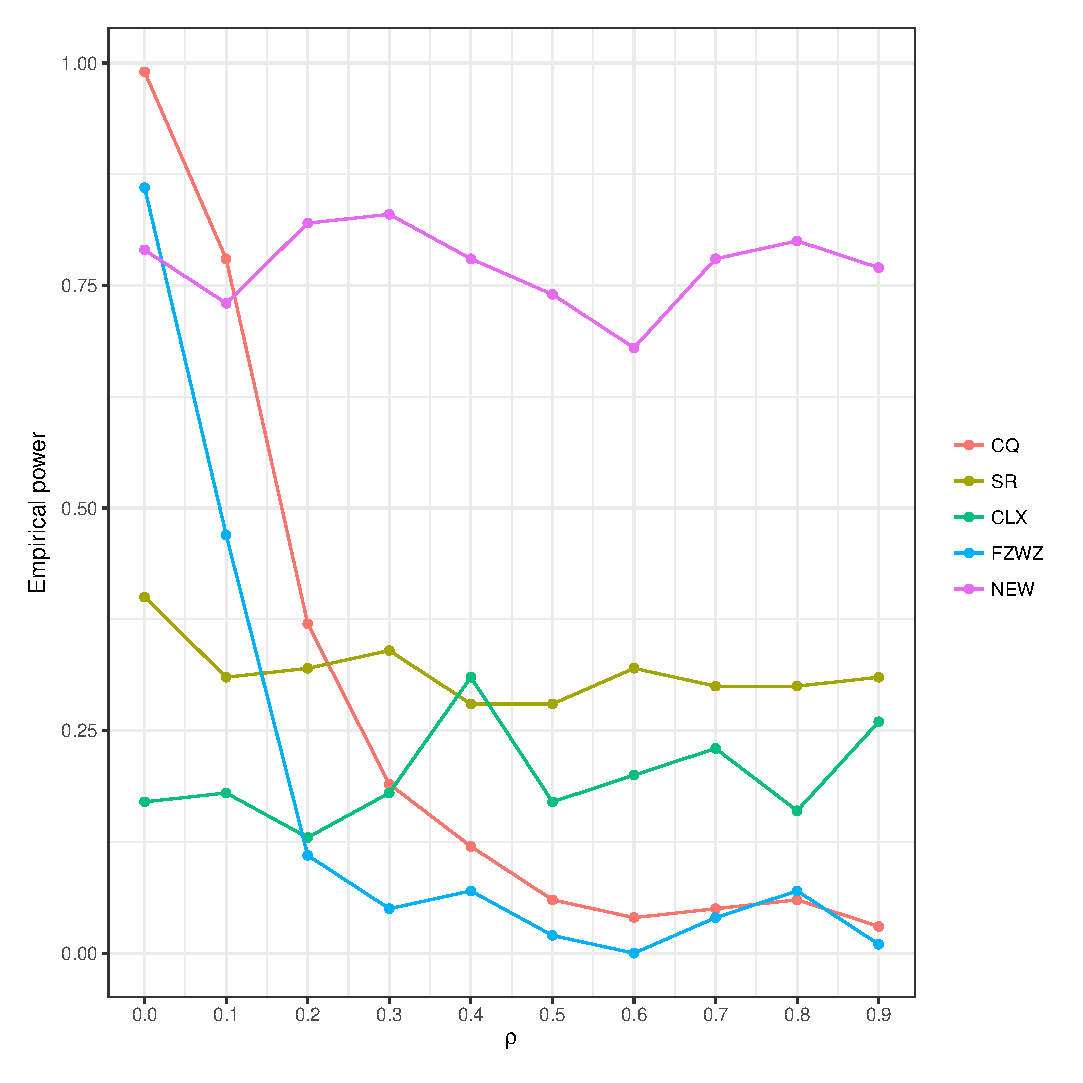
\includegraphics[width=12cm,height=12cm]{figure1}
    \caption{The empirical powers of tests. $\alpha=0.05$, $k=2$, $n_1=n_2=20$, $p=150$.}\label{figure1}
\end{figure}




%\begin{table}[!hbp]
%    \caption{Empirical powers of tests under covariance structure II and non-sparse alternative. $\alpha=0.05$, $k=3$, $n_1=n_2=n_3=25$. }
%    \label{table5}
%    \centering
%\begin{tabular}{*{10}{c}}
%\toprule
%\multirow{2}{*}{SNR} &\multicolumn{3}{c}{$p=100$}&\multicolumn{3}{c}{$p=150$}&\multicolumn{3}{c}{$p=200$} \\
%    \cmidrule(r){2-4}\cmidrule(r){5-7}\cmidrule(r){8-10}
%        & CX & SC & LFD & CX &SC &LFD &CX & SC & LFD\\
%\midrule
%0 & 0.063 & 0.054 & 0.058 & 0.052 & 0.040 & 0.042 & 0.045 & 0.049 & 0.070 \\ 
%1 & 0.141 & 0.120 & 0.115 & 0.126 & 0.120 & 0.112 & 0.103 & 0.110 & 0.102 \\ 
%2 & 0.181 & 0.209 & 0.169 & 0.330 & 0.260 & 0.210 & 0.200 & 0.227 & 0.201 \\ 
%3 & 0.692 & 0.367 & 0.244 & 0.759 & 0.385 & 0.341 & 0.468 & 0.413 & 0.394 \\ 
%4 & 0.753 & 0.539 & 0.420 & 0.744 & 0.573 & 0.515 & 0.516 & 0.554 & 0.561 \\ 
%5 & 0.828 & 0.690 & 0.509 & 0.871 & 0.697 & 0.693 & 0.556 & 0.724 & 0.727 \\ 
%6 & 0.809 & 0.812 & 0.622 & 0.822 & 0.824 & 0.766 & 0.959 & 0.838 & 0.859 \\ 
%7 & 1.000 & 0.882 & 0.780 & 0.979 & 0.916 & 0.903 & 0.990 & 0.923 & 0.947 \\ 
%8 & 0.993 & 0.955 & 0.789 & 1.000 & 0.965 & 0.954 & 0.999 & 0.972 & 0.971 \\ 
%9 & 1.000 & 0.979 & 0.911 & 0.999 & 0.981 & 0.979 & 0.964 & 0.986 & 0.987 \\ 
%10 & 1.000 & 0.991 & 0.877 & 0.989 & 0.996 & 0.988 & 0.996 & 0.996 & 0.997 \\ 
%\bottomrule
%\end{tabular}
%\end{table}

%\begin{table}[!hbp]
%    \caption{Empirical powers of tests under covariance structure II and sparse alternative. $\alpha=0.05$, $k=3$, $n_1=n_2=n_3=25$. }
%    \label{table6}
%    \centering
%\begin{tabular}{*{10}{c}}
%\toprule
%\multirow{2}{*}{SNR} &\multicolumn{3}{c}{$p=100$}&\multicolumn{3}{c}{$p=150$}&\multicolumn{3}{c}{$p=200$} \\
%    \cmidrule(r){2-4}\cmidrule(r){5-7}\cmidrule(r){8-10}
%        & CX & SC & LFD & CX &SC &LFD &CX & SC & LFD\\
%\midrule
%0 & 0.052 & 0.055 & 0.047 & 0.055 & 0.057 & 0.053 & 0.044 & 0.055 & 0.057 \\ 
%1 & 0.068 & 0.124 & 0.065 & 0.070 & 0.130 & 0.085 & 0.049 & 0.116 & 0.087 \\ 
%2 & 0.085 & 0.233 & 0.112 & 0.076 & 0.239 & 0.149 & 0.067 & 0.241 & 0.161 \\ 
%3 & 0.110 & 0.388 & 0.161 & 0.090 & 0.408 & 0.215 & 0.097 & 0.417 & 0.227 \\ 
%4 & 0.120 & 0.530 & 0.184 & 0.112 & 0.552 & 0.282 & 0.103 & 0.556 & 0.309 \\ 
%5 & 0.167 & 0.708 & 0.238 & 0.142 & 0.699 & 0.387 & 0.140 & 0.687 & 0.394 \\ 
%6 & 0.196 & 0.807 & 0.261 & 0.168 & 0.820 & 0.472 & 0.162 & 0.823 & 0.547 \\ 
%7 & 0.217 & 0.875 & 0.318 & 0.177 & 0.892 & 0.505 & 0.173 & 0.896 & 0.646 \\ 
%8 & 0.234 & 0.935 & 0.378 & 0.220 & 0.951 & 0.625 & 0.195 & 0.948 & 0.749 \\ 
%9 & 0.312 & 0.965 & 0.407 & 0.222 & 0.970 & 0.672 & 0.224 & 0.979 & 0.809 \\ 
%10 & 0.334 & 0.976 & 0.505 & 0.292 & 0.987 & 0.773 & 0.254 & 0.989 & 0.881 \\ 
%\bottomrule
%\end{tabular}
%\end{table}

\section{Concluding remarks}\label{concluding}
In this paper, using the idea of least favorable direction, we proposed LFD test for MANOVA in high dimensional setting.
We derived the asymptotic distribution of LFD test statistic. We also gave the asymptotic local power function.
Our theoretic work and simulation studies show that when the covariance matrix is spiked, LFD test tends to be more powerful than existing tests.

Our proof relies on the normality of the observations.
It is interesting to investigate whether the theorems are still valid without normal assumption.
Moreover, we assumed that $p$ doesn't grow too fast.
 Without prior knowledge of $\Sigma$, this condition is unavoidable since when $p$ is large, it's impossible to consistently estimate the principal space.
See, for example,~\cite{Cai2012Sparse}.
On the other hand, if we know some prior knowledge of $\Sigma$, for example, $\Sigma$ is sparse, it's possible to construct a better test.
We leave it for future research.


%In Section~\label{sc:compare}, we consider a random projection test.
%The theoretical properties of random projection test may be a.





\begin{appendices}
    \section{Technical details}\label{app}

\begin{proposition}\label{optProp}
    Suppose $\bA$ is a $p\times r$ matrix with rank $r$ and $\bB$ is a $p\times p$  non-zero positive semi-definite matrix.
    Denote by $\bA=\bU_\bA \bD_\bA \bV_\bA^T$ the singular value decomposition of $\bA$, where $\bU_\bA$ and $\bV_\bA$ are $p\times r$ and $r\times r$ column orthogonal matrix, $\bD_\bA$ is a $r\times r$ diagonal matrix.
    Let $\bP_\bA=\bU_\bA \bU_\bA^T$ be the projection matrix on the column space of $\bA$.
    Then
    \begin{equation}
        \max_{a^T a=1, a^T \bA \bA^T a=0}a^T \bB a=
        \lambda_{\max}\big(\bB(\bI_p-\bP_\bA)\big).
    \end{equation}
\end{proposition}
\begin{proof}
    Note that $a^T \bA \bA^T a=0$ is equivalent to $\bP_\bA a=0$ which in turn is equivalent to $a= (\bI_p-\bP_\bA)a$.
    Then
    \begin{equation}\label{eq:prop1eq1}
        \begin{aligned}
        \max_{a^T a=1, a^T \bA \bA^T a=0}a^T \bB a
            &=
        \max_{a^T a=1, \bP_\bA a=0}a^T(\bI_p-\bP_\bA) \bB (\bI_p-\bP_\bA)a,
        \end{aligned}
    \end{equation}
    which is obviously no greater than $\lambda_{\max}\big((\bI-\bP_\bA)\bB(\bI-\bP_\bA)\big)$.
    To prove that they are equal,  without loss of generality, we can assume $\lambda_{\max}\big((\bI-\bP_\bA)\bB(\bI-\bP_\bA)\big)>0$.
    Let $\alpha_1$ be one eigenvector corresponding to the largest eigenvalue of $(\bI-\bP_\bA)\bB(\bI-\bP_\bA)$.
    Since $(\bI-\bP_\bA)\bB(\bI-\bP_\bA)\bP_\bA=(\bI-\bP_\bA)\bB(\bP_\bA-\bP_\bA)=\bO_{p\times p}$ and $\bP_\bA$ is symmetric, the rows of $\bP_\bA$ are eigenvetors of $(\bI-\bP_\bA)\bB(\bI-\bP_\bA)$ corresponding to eigenvalue $0$.
    It follows that $\bP_\bA\alpha_1=0$.
    Therefore, $\alpha_1$ satisfies the constraint of~\eqref{eq:prop1eq1} and~\eqref{eq:prop1eq1} is no less than $\lambda_{\max}\big((\bI-\bP_\bA)\bB(\bI-\bP_\bA)\big)$.
    The conclusion now follows by noting that $\lambda_{\max}\big((\bI-\bP_\bA)\bB(\bI-\bP_\bA)\big)=\lambda_{\max}\big( \bB(\bI-\bP_\bA)\big)$.
    
\end{proof}
    \begin{lemma}[Weyl's inequality]
        Let $\bA$ and $\bB$ be two symmetric $n\times n$ matrices. If $r+s-1\leq i \leq j+k-n$, we have
        $$
        \lambda_j(\bA) +\lambda_k(\bB)\leq \lambda_i (\bA+\bB) \leq
        \lambda_r(\bA)+\lambda_s(\bB).
        $$
        See, for example,~\citet{Horn1985Matrix} Theorem 4.3.1.
\end{lemma}
%\begin{lemma}[\citet{DAVIDSON2001317} Theorem II.7]\label{DSbound}
    %Let $\bA$ be $m\times n$ random matrix with iid $\mathcal{N}(0,1)$ entries.
    %If $m>n$, then for any $t>0$,
    %\begin{align*}
        %\Pr(\sqrt{\lambda_1(\bA \bA^T)}>\sqrt{m}+\sqrt{n}+t)\leq \exp(-t^2/2),\\
        %\Pr(\sqrt{\lambda_n(\bA \bA^T)}<\sqrt{m}-\sqrt{n}-t)\leq \exp(-t^2/2).
    %\end{align*}
%\end{lemma}

\begin{lemma}\label{lemma:con}
    Let $\{Z_i\}_{i=1}^n$ be iid $p$-dimensional random vectors with common distribution $\mathcal{N}_p(\mathbf{0}_p,\bI_p)$.
    Then for any $n$-dimensional vector $\omega=(\omega_1,\ldots,\omega_n)^T$, we have
\begin{equation*}
    \left\|\sum_{i=1}^n \omega_i(Z_i Z_i^T - \bI_p)\right\|=O_P(|\omega|_2 \sqrt{p}+|\omega|_{\infty}p).
\end{equation*}
\end{lemma}
\begin{proof}
    This proof is adapted from the proof of Theorem 5.39 in~\cite{Vershynin2010Introduction}.
    By Lemma 5.2 and Lemma 5.4 of~\cite{Vershynin2010Introduction}, there exists a set $\mathcal{C}\subset \{x\in\mathbb{R}^p: |x|_2=1\}$ satisfying $\text{Card} (\mathcal{C})\leq 9^p$ such that for any $p\times p$ symmetric matrix $\bA$,
    \begin{equation}\label{eq:b1}
    \|A\|\leq 2\max_{x\in\mathcal{C}} x^T \bA x.
\end{equation}
For $t>1$, we have
\begin{equation*}
    \begin{split}
        &\Pr\left(
            \left\|\sum_{i=1}^n \omega_i(Z_i Z_i^T - \bI_p)\right\|
            > t (|\omega|_2 \sqrt{p}+|\omega|_{\infty} p)
        \right)
        \\
        \leq &
        \Pr\left(
            2\sup_{x\in\mathcal{C}}\left|\sum_{i=1}^n \omega_i(x^T Z_i Z_i^T x - 1)\right|
            > t (|\omega|_2 \sqrt{p}+|\omega|_{\infty} p)
        \right)
        \\
        \leq &
        \sum_{x\in\mathcal{C}}
        \Pr\left(
            \left|\sum_{i=1}^n \omega_i(x^T Z_i Z_i^T x - 1)\right|
            >  |\omega|_2 \sqrt{\frac{pt}{4}}+2|\omega|_{\infty} \frac{pt}{4}
        \right)
        \\
        \leq & 2\cdot 9^{p} \exp\left(-\frac{pt}{4}\right)
        =2\exp\left((2\log 3 -t/4)p\right)
        \leq 2\exp\left(2\log 3 -t/4\right)
        ,
    \end{split}
\end{equation*}
where the first inequality follows from~\eqref{eq:b1}, the second inequality follows from union bound and the third inequality follows Lemma 1 of~\cite{Laurent2000Adaptive}.
The upper bound $2\exp\left(2\log 3 -t/4\right)$ can be arbitrarily small as long as $t$ is large enough.
This completes the proof.
\end{proof}

We can write $\bY=\bU\bLambda^{1/2}\bZ$, where $\bZ$ be a $p\times n$ random matrix with iid standard normal entries.
    Let $\bZ =(\bZ_1^T,\bZ_2^T)^T$, where $\bZ_1$ and $\bZ_2$ are the first $r$ rows and last $p-r$ rows of $\bZ$.
    Let $\hat{\bSigma}=n^{-1}\bY\bY^T$.
\begin{proposition}
    \label{eigenvalueProp}
    Suppose that $r\leq n$.
    Then uniformly for $i=1,\ldots, r$, 
\begin{equation}\label{eigenvalueProp:R1}
        %\lambda_i\left(n^{-1}\bZ^T \bLambda \bZ\right)
    \lambda_i(\hat{\bSigma})
        =
        \blambda_i
        +
        n^{-1}\sum_{i=r+1}^p\blambda_i
        +O_P\left(\blambda_i \sqrt{\frac{r}{n}}+\sqrt{\frac{\mytr(\bLambda_2^2)}{ n}}+\blambda_{r+1}\right).
    \end{equation}
And 
\begin{equation}\label{eigenvalueProp:R2}
    \begin{split}
     &\sum_{i=r+1}^p\lambda_i(\hat{\bSigma})
    =
\mytr(\bLambda_2)
    -
    \frac{r}{n}\sum_{i=r+1}^p \blambda_i
    +O_P\left(r\sqrt{\frac{\mytr(\bLambda_2^2)}{ n}}+r\blambda_{r+1}\right)
    .
    \end{split}
\end{equation}
\end{proposition}
\begin{proof}
    We only need to deal with the matrix $n^{-1}\bZ^T \bLambda \bZ$ since it shares the same non-zero eigenvalues as $\hat{\bSigma}$.
    Write
    \begin{equation*}
        \begin{split}
        n^{-1}\bZ^T \bLambda \bZ=&
        n^{-1}\bZ_1^T \bLambda_1 \bZ_1+
        n^{-1}\bZ_2^T \bLambda_2 \bZ_2
        \\
        =&
        n^{-1}\bZ_1^T \bLambda_1 \bZ_1+
        n^{-1}(\sum_{i=r+1}^p\blambda_i)\bI_n+
        n^{-1}\left(\bZ_2^T \bLambda_2 \bZ_2-(\sum_{i=r+1}^p\blambda_i)\bI_n\right)
        .
        \end{split}
    \end{equation*}
    Then Weyl's inequality implies that for $ i=1,\ldots, r$,
    \begin{equation}\label{eigenBoundForF}
        \begin{split}
        &
        \left|
        \lambda_i\left(n^{-1}\bZ^T \bLambda \bZ\right)
        -
        \lambda_i(n^{-1}\bZ_1^T \bLambda_1 \bZ_1)
        -
        n^{-1}\sum_{i=r+1}^p\blambda_i
        \right|
        \leq
        n^{-1}\left\|\bZ_2^T \bLambda_2 \bZ_2-(\sum_{i=r+1}^p\blambda_i)\bI_n\right\|.
        \end{split}
    \end{equation}
    Using Weyl's inequality, we can derive the following lower bound for $\lambda_i(n^{-1}\bZ_1^T \bLambda_1 \bZ_1)$, $ i=1,\ldots, r$.
\begin{equation*}\label{eq:DLower}
\begin{aligned}
\lambda_i(\bZ_1^T \bLambda_1 \bZ_1)
\geq&
\lambda_i(\bZ_1^T \mydiag(\blambda_i \bI_{i},\bO_{(r-i)\times(r-i)}) \bZ_1)
\\
    =&
    \lambda_i\Big( \blambda_i \bZ_1^T \bZ_1-\blambda_i\bZ_1^T \mydiag(\bO_{i\times i}, \bI_{r-i}) \bZ_1\Big)\\
    \geq&
    \lambda_r\Big( \blambda_i \bZ_1^T \bZ_1\Big)+\lambda_{n+i-r}\Big(-\blambda_i\bZ_1^T \mydiag(\bO_{i\times i}, \bI_{r-i}) \bZ_1\Big)\\
= &
\blambda_i \lambda_r(\bZ_1\bZ_1^T).
\end{aligned}
\end{equation*}
Similarly, we can derive the following upper bound for
$\lambda_i(\bZ_1^T \bLambda_1 \bZ_1)$, $i=1,\ldots,r$.
\begin{equation*}\label{eq:DUpper}
\begin{aligned}
&\lambda_i(\bZ_1^T \bLambda_1 \bZ_1)
\\
=&\lambda_i\Big(
\bZ_1^T \big(
\mydiag(\blambda_1,\ldots,\blambda_{i-1},\bO_{(r-i+1)\times(r-i+1)})+
\mydiag(\bO_{(i-1)\times(i-1)},\blambda_i,\ldots,\blambda_r)
\big)
\bZ_1
\Big)\\
%\leq&
%\lambda_1(\bZ_{1[1:r,:]}^T \mydiag(\bO_{(i-1)\times(i-1)},\lambda_i,\ldots,\lambda_r) \bZ_{1[1:r,:]})
    \leq&
\lambda_1(\bZ_1^T \mydiag(\bO_{(i-1)\times(i-1)},\blambda_i \bI_{r-i+1}) \bZ_1)
\leq  \blambda_i \lambda_1(\bZ_1\bZ_1^T).
\end{aligned}
\end{equation*}
The above lower bound and upper bound imply
\begin{equation}\label{eigenBoundForA}
    \begin{aligned}
\left|
\lambda_i(n^{-1}\bZ_1^T \bLambda_1 \bZ_1)-\blambda_i
\right|
\leq&
\blambda_i 
\max\left(
    |\lambda_1(n^{-1}\bZ_1 \bZ_1^T)-1|,
    |\lambda_r(n^{-1}\bZ_1 \bZ_1^T)-1|
\right)
\\
=&\blambda_i \|n^{-1}\bZ_1\bZ_1^T -\bI_r\|.
    \end{aligned}
\end{equation}
Combining the bounds~\eqref{eigenBoundForF} and~\eqref{eigenBoundForA} gives that for $i=1,\ldots,r$,
\begin{equation*}
    \begin{split}
        &
        \left|
        \lambda_i\left(n^{-1}\bZ^T \bLambda \bZ\right)
        -
        \blambda_i
        -
        n^{-1}\sum_{i=r+1}^p\blambda_i
        \right|
        \\
        \leq&
        n^{-1}\left\|\bZ_2^T \bLambda_2 \bZ_2-(\sum_{i=r+1}^p\blambda_i)\bI_n\right\|
        +\blambda_i \|n^{-1}\bZ_1\bZ_1^T -\bI_r\|.
    \end{split}
\end{equation*}
    By Lemma~\ref{lemma:con}, we have
\begin{align}
    \label{conB2B1}
            \|n^{-1}\bZ_1\bZ_1^T -\bI_r\|&=
            O_P\left(\sqrt{\frac{r}{n}}\right),
        \\
        \label{conB2B}
        n^{-1}\left\|\bZ_2^T \bLambda_2 \bZ_2-(\sum_{i=r+1}^p\blambda_i)\bI_n\right\|&=O_P\left(\sqrt{\frac{\mytr(\bLambda_2^2)}{ n}}+\blambda_{r+1}\right).
\end{align}
Then~\eqref{eigenvalueProp:R1} follows.

To prove~\eqref{eigenvalueProp:R2}, we note that
\begin{equation*}
    \begin{split}
     \sum_{i=r+1}^p\lambda_i(\hat{\bSigma})
    =&
    \sum_{i=r+1}^n\lambda_i(n^{-1}\ \bZ^T \bLambda \bZ)
    \\
    =&
    \mytr (n^{-1}\bZ^T \bLambda \bZ) -\sum_{i=1}^r\lambda_i(n^{-1}\ \bZ^T \bLambda \bZ)
    \\
    =&
    \mytr (n^{-1}\bZ_1^T \bLambda_1 \bZ_1)
    +
    \mytr (n^{-1}\bZ_2^T \bLambda_2 \bZ_2)
    -\sum_{i=1}^r\lambda_i(n^{-1}\ \bZ^T \bLambda \bZ)
    .
    \end{split}
\end{equation*}
It follows from inequalities~\eqref{eigenBoundForF} and~\eqref{conB2B} that
\begin{equation*}
    \begin{split}
    &\left|
    \sum_{i=1}^r\lambda_i(n^{-1}\ \bZ^T \bLambda \bZ)
    -\mytr (n^{-1}\bZ_1^T \bLambda_1 \bZ_1)- \frac{r}{n}\sum_{i=r+1}^p \blambda_i
    \right|
    \\
    \leq & \frac{r}{n}
    \left\|\bZ_2^T \bLambda_2 \bZ_2-(\sum_{i=r+1}^p\blambda_i)\bI_n\right\|
    =
    O_P\left(
    r\sqrt{\frac{\mytr(\bLambda_2^2)}{ n}}+r\blambda_{r+1}
    \right)
    .
    \end{split}
\end{equation*}
Thus,
\begin{equation*}
        \sum_{i=r+1}^p\lambda_i(\hat{\bSigma})
    =
    \mytr (n^{-1}\bZ_2^T \bLambda_2 \bZ_2)
    -
    \frac{r}{n}\sum_{i=r+1}^p \blambda_i
    +O_P\left(
    r\sqrt{\frac{\mytr(\bLambda_2^2)}{ n}}+r\blambda_{r+1}
    \right)
    .
\end{equation*}
It is straightforward to show that
\begin{equation*}
    \myE \mytr (n^{-1}\bZ_2^T \bLambda_2 \bZ_2)=\mytr(\bLambda_2),
    \quad
    \myVar \left(\mytr (n^{-1}\bZ_2^T \bLambda_2 \bZ_2)\right)
    =\frac{2}{n}\mytr(\bLambda_2^2).
\end{equation*}
Hence
\begin{equation*}
    \begin{split}
     &\sum_{i=r+1}^p\lambda_i(\hat \bSigma)
     \\
    =&
\mytr(\bLambda_2)+O_P\left(\sqrt{\frac{\mytr(\bLambda_2^2)}{ n}}\right)
    -
    \frac{r}{n}\sum_{i=r+1}^p \blambda_i
    +O_P\left(
    r\sqrt{\frac{\mytr(\bLambda_2^2)}{ n}}+r\blambda_{r+1}
\right)
     \\
    =&
\mytr(\bLambda_2)
    -
    \frac{r}{n}\sum_{i=r+1}^p \blambda_i
    +O_P\left(
    r\sqrt{\frac{\mytr(\bLambda_2^2)}{ n}}+r\blambda_{r+1}
\right)
    .
    \end{split}
\end{equation*}
This completes the proof of~\eqref{eigenvalueProp:R2}.

\end{proof}

\begin{proposition}\label{newEigenvectorProp}
    Suppose that $p>n$, $r=o(n)$ and $r\blambda_{r+1} /\mytr(\bLambda_2)\to 0$. Then
    \begin{equation*}
        \|\bU_{\bY,1}\bU_{\bY,1}^T -\bP_{\bY,1}^* \|
        =O_P\left(\frac{\blambda_{r+1}+n^{-1}\mytr(\bLambda_2)}{\blambda_r +n^{-1}\mytr(\bLambda_2)}\right),
    \end{equation*}
    where
    \begin{equation*}
        \bP_{\bY,1}^*=
    \bU
    \begin{pmatrix}
       \bI_r \\
       \bQ
    \end{pmatrix}
    \left(\bI_r+ n^{-1}\mytr(\bLambda_2)\bLambda_1^{-1}\right)^{-1}
    \begin{pmatrix}
        \bI_r
          &
          \bQ^T
        \end{pmatrix}
        \bU^T.
    \end{equation*}
\end{proposition}
\begin{proof}
    The following intermediate matrix
    \begin{equation*}
        \begin{split}
    \hat{\bSigma}_0 =&
    n^{-1}\bU_1 \bLambda_1^{1/2} \bZ_1 \bZ_1^T \bLambda_1^{1/2}\bU_1^T
    +n^{-1}\bU_1 \bLambda_1^{1/2} \bZ_1 \bZ_2^T \bLambda_2^{1/2}\bU_2^T
    +n^{-1}\bU_2 \bLambda_2^{1/2} \bZ_2 \bZ_1^T \bLambda_1^{1/2}\bU_1^T
    \\
    &+n^{-1}\bU_2 \bLambda_2^{1/2} \bZ_2 \bZ_1^T 
    ( \bZ_1 \bZ_1^T )^{-1}
    \bZ_1
    \bZ_2^T \bLambda_2^{1/2}\bU_2^T
        \end{split}
    \end{equation*}
    plays a key role in the proof.
    It can be seen that 
    \begin{equation*}
        \hat{\bSigma}_0=n^{-1}
    \bU
    \begin{pmatrix}
       \bI_r \\
       \bQ
    \end{pmatrix}
    \bLambda_1^{1/2}\bZ_1 \bZ_1^T\bLambda_1^{1/2}
    \begin{pmatrix}
        \bI_r
          &
          \bQ^T
        \end{pmatrix}
        \bU^T,
    \end{equation*}
    where
    $
       \bQ=
       \bLambda_2^{1/2} \bZ_2 \bZ_1^T (\bZ_1 \bZ_1^T)^{-1} \bLambda_1^{-1/2}
       $.
    Consequently, $\hat{\bSigma}_0$ is a positive semi-definite matrix with rank $r$, and 
    %the columns of
    %\begin{equation*}
    %\bU
    %\begin{pmatrix}
       %\bI_r \\
       %\bQ
   %\end{pmatrix}
    %\end{equation*}
    %spans the rank $r$ principal subspace of $\hat{\bSigma}_0$.
    %Hence
    the matrix
    \begin{equation*}
        \begin{split}
        \bP_0
        =&
    \bU
    \begin{pmatrix}
       \bI_r \\
       \bQ
    \end{pmatrix}
    \left(
        \bI_r+\bQ^T \bQ
    \right)^{-1}
    \begin{pmatrix}
        \bI_r
          &
          \bQ^T
        \end{pmatrix}
        \bU^T
        \end{split}
    \end{equation*}
    is the projection matrix onto the rank $r$ principal subspace of $\hat{\bSigma}_0$.

    From~\cite{Cai2015Optimal}, Proposition 1, we have
    \begin{equation}\label{asd1}
        \|\bU_{\bY,1}\bU_{\bY,1}^T -\bP_0 \|
        \leq 
        \frac{2\|\hat{\bSigma}-\hat{\bSigma}_0\|}{\lambda_r(\hat{\bSigma}_0)}.
    \end{equation}
    We have the following upper bound for $\|\hat{\bSigma}-\hat{\bSigma}_0\|$.
    \begin{equation}\label{asd2}
        \begin{split}
            \|\hat{\bSigma}-\hat{\bSigma}_0\|
            =&
    n^{-1}\left\|\bU_2 \bLambda_2^{1/2} \bZ_2  
    \bZ_2^T \bLambda_2^{1/2}\bU_2^T
    -\bU_2 \bLambda_2^{1/2} \bZ_2 \bZ_1^T 
    ( \bZ_1 \bZ_1^T )^{-1}
    \bZ_1
    \bZ_2^T \bLambda_2^{1/2}\bU_2^T
    \right\|
    \\
    \leq &
    n^{-1}\left\| \bLambda_2^{1/2} \bZ_2  
    \bZ_2^T \bLambda_2^{1/2}\right\|
    +n^{-1}\left\|\bLambda_2^{1/2} \bZ_2 \bZ_1^T 
    ( \bZ_1 \bZ_1^T )^{-1}
    \bZ_1
    \bZ_2^T \bLambda_2^{1/2}
    \right\|
    \\
    \leq &
    2n^{-1}\left\|\bZ_2^T \bLambda_2 \bZ_2\right\|
    \\
 \leq& 
     2n^{-1}\left\| \bZ_2^T \bLambda_2\bZ_2-\mytr(\bLambda_2)\bI_n\right\|
     +n^{-1}
     \mytr(\bLambda_2)
     \\
     =&O_P\left( 
\sqrt{\frac{\mytr\left(\bLambda_2^2\right)}{n}}+\blambda_{r+1}
     +
     n^{-1}\mytr(\bLambda_2)
 \right)
 \\
     =&O_P\left( 
\blambda_{r+1}
     +
     n^{-1}\mytr(\bLambda_2)
 \right)
 ,
    \end{split}
\end{equation}
where
the second last equality follows from~\eqref{conB2B} and the last equality follows from
\begin{equation*}
    \sqrt{\frac{\mytr\left(\bLambda_2^2\right)}{n}}
    \leq
    \sqrt{\frac{\blambda_{r+1}\mytr\left(\bLambda_2\right)}{n}}
    \leq
    \frac{1}{2}\left(\blambda_{r+1}+n^{-1}\mytr\left(\bLambda_2\right)\right).
\end{equation*}
Now we deal with $\lambda_r(\hat{\bSigma}_0)$.
We have
\begin{equation*}
    \begin{split}
     \lambda_r(\hat{\bSigma}_0)
     =&\lambda_r\left(
n^{-1}
         \bZ_1^T \bLambda_1^{1/2}(\bI_r +\bQ^T \bQ)\bLambda_1^{1/2} \bZ_1
     \right)
     \\
     =&\lambda_r\left(
n^{-1}
          \bLambda_1^{1/2}(\bI_r +\bQ^T \bQ)\bLambda_1^{1/2} \bZ_1\bZ_1^T
     \right)
     \\
     =&\lambda_r\left(
n^{-1}
  (\bZ_1\bZ_1^T)^{1/2}\bLambda_1^{1/2}(\bI_r +\bQ^T \bQ)\bLambda_1^{1/2} (\bZ_1\bZ_1^T)^{1/2}
     \right)
     \\
     =&
     \lambda_r\left(
        n^{-1} (\bZ_1\bZ_1^T)^{1/2}
         \bLambda_1 
         (\bZ_1\bZ_1^T)^{1/2}
         +
        n^{-1} (\bZ_1 \bZ_1^T)^{-1/2} \bZ_1 \bZ_2^T \bLambda_2 \bZ_2 \bZ_1^T (\bZ_1 \bZ_1^T)^{-1/2} 
    \right).
    \end{split}
\end{equation*}
It can be seen that $\bZ_2 \bZ_1^T (\bZ_1 \bZ_1^T)^{-1/2}$ is a $(p-r)\times r$ random matrix with iid $\mathcal{N}(0,1)$ entries.
Then Lemma~\ref{lemma:con} implies that
\begin{equation}\label{projCon}
        \begin{split}
        &\left\|n^{-1} (\bZ_1 \bZ_1^T)^{-1/2} \bZ_1 \bZ_2^T \bLambda_2 \bZ_2 \bZ_1^T (\bZ_1 \bZ_1^T)^{-1/2} 
        -n^{-1} \mytr(\bLambda_2) \bI_r
        \right\|
        \\
        =&
        O_P\left(
            n^{-1}\sqrt{r\mytr\left(\bLambda_2^2\right)}
            +rn^{-1}\blambda_{r+1}
        \right)
        \\
        =&
        O_P\left(
            n^{-1}\sqrt{r\blambda_{r+1}\mytr\left(\bLambda_2\right)}
            +rn^{-1}\blambda_{r+1}
        \right)
        \\
        =&o_P\left(n^{-1}\mytr(\bLambda_2)\right)
        ,
        \end{split}
    \end{equation}
    where the last equality follows from the condition $r\blambda_{r+1} /\mytr(\bLambda_2)\to 0$.
    Then it follows from Weyl's inequality that 
    \begin{equation*}
        \begin{split}
        &\left| 
        \lambda_r (\hat{\bSigma}_0)-
     \lambda_r\left(
        n^{-1} (\bZ_1\bZ_1^T)^{1/2}
         \bLambda_1 
         (\bZ_1\bZ_1^T)^{1/2}
         +
         n^{-1} \mytr(\bLambda_2)\bI_r 
    \right)
    \right|
\\
        \leq &\left\|n^{-1} (\bZ_1 \bZ_1^T)^{-1/2} \bZ_1 \bZ_2^T \bLambda_2 \bZ_2 \bZ_1^T (\bZ_1 \bZ_1^T)^{-1/2} 
        -n^{-1} \mytr(\bLambda_2) \bI_r
        \right\|
        \\
        =&o_P\left(n^{-1}\mytr(\bLambda_2)\right).
        \end{split}
    \end{equation*}
    On the other hand,~\eqref{eigenBoundForA} and~\eqref{conB2B1} imply that
    \begin{equation*}
        \begin{split}
        &
     \lambda_r\left(
        n^{-1} (\bZ_1\bZ_1^T)^{1/2}
         \bLambda_1 
         (\bZ_1\bZ_1^T)^{1/2}
         +
         n^{-1} \mytr(\bLambda_2)\bI_r 
    \right)
\\
        =&
     \lambda_r\left(
        n^{-1} \bZ_1^T
         \bLambda_1 
         \bZ_1
    \right)
         +
         n^{-1} \mytr(\bLambda_2)
        \\
        =&
        \blambda_r +o_P(\blambda_r)
         +
         n^{-1} \mytr(\bLambda_2).
        \end{split}
    \end{equation*}
    Hence we have 
    \begin{equation}\label{asd3}
    \lambda_r(\hat{\bSigma}_0)=(1+o_P(1))(\blambda_r+n^{-1}\mytr(\bLambda_2)).
    \end{equation}
    Combining~\eqref{asd1},~\eqref{asd2} and~\eqref{asd3} yields
    \begin{equation*}
        \|\bU_{\bY,1}\bU_{\bY,1}^T -\bP_0 \|
        =O_P\left(\frac{\blambda_{r+1}+n^{-1}\mytr(\bLambda_2)}{\blambda_r +n^{-1}\mytr(\bLambda_2)}\right).
    \end{equation*}

    Now we deal with $\bP_0$.
    By some algebra, we have
    \begin{equation*}
        \begin{split}
        &\Big\|\bP_0
        -
        \bP_{\bY,1}^*
        \Big\|
        \\
        = &
        \left\|
\left(\bI_r+ \bQ^T \bQ \right)^{1/2}
        \left(
    \left(\bI_r+ \bQ^T \bQ \right)^{-1}
-
    \left(\bI_r+ n^{-1}\mytr(\bLambda_2)\bLambda_1^{-1}\right)^{-1}
\right)
\left(\bI_r+ \bQ^T \bQ \right)^{1/2}
        \right\|
        \\
        = &
        \left\|
        \bI_r-
\left(\bI_r+ \bQ^T \bQ \right)^{1/2}
    \left(\bI_r+ n^{-1}\mytr(\bLambda_2)\bLambda_1^{-1}\right)^{-1}
\left(\bI_r+ \bQ^T \bQ \right)^{1/2}
        \right\|
        \\
        = &
        \left\|
        \bI_r-
    \left(\bI_r+ n^{-1}\mytr(\bLambda_2)\bLambda_1^{-1}\right)^{-1/2}
\left(\bI_r+ \bQ^T \bQ \right)
    \left(\bI_r+ n^{-1}\mytr(\bLambda_2)\bLambda_1^{-1}\right)^{-1/2}
        \right\|
        \\
        = &
        \left\|
    \left(\bI_r+ n^{-1}\mytr(\bLambda_2)\bLambda_1^{-1}\right)^{-1/2}
    \left(\bQ^T \bQ-n^{-1}\mytr(\bLambda_2) \bLambda_1^{-1} \right)
    \left(\bI_r+ n^{-1}\mytr(\bLambda_2)\bLambda_1^{-1}\right)^{-1/2}
        \right\|
        \\
        =&
        \left\|
        \left(\bLambda_1+n^{-1}\mytr(\bLambda_2)\right)^{-1/2}
        \left(
            %(\bZ_1 \bZ_1^T)^{-1}
            %\bZ_1 \bZ_2^T \bLambda_2 \bZ_2 \bZ_1^T 
            %(\bZ_1 \bZ_1^T)^{-1}
            \bLambda_1^{1/2}\bQ^T \bQ \bLambda_1^{1/2}
            - n^{-1} \mytr(\bLambda_2) \bI_r
        \right)
        \left(\bLambda_1+n^{-1}\mytr(\bLambda_2)\right)^{-1/2}
        \right\|
        .
        \end{split}
    \end{equation*}
    Thus,
    \begin{equation*}
        \begin{split}
        &
        \left\|
        \bP_0-\bP_{\bY,1}^*
        \right\|
        \\
        \leq &
        \left(\blambda_r+n^{-1}\mytr(\bLambda_2)\right)^{-1}
        \left\|
            (\bZ_1 \bZ_1^T)^{-1}
            \bZ_1 \bZ_2^T \bLambda_2 \bZ_2 \bZ_1^T 
            (\bZ_1 \bZ_1^T)^{-1}
            - n^{-1} \mytr(\bLambda_2) \bI_r
        \right\|
        \\
        \leq &
        \left(\blambda_r+n^{-1}\mytr(\bLambda_2)\right)^{-1}
        \left\|
            (\bZ_1 \bZ_1^T)^{-1}
            \bZ_1 \bZ_2^T \bLambda_2 \bZ_2 \bZ_1^T 
            (\bZ_1 \bZ_1^T)^{-1}
        -
        \mytr(\bLambda_2)  \left(\bZ_1 \bZ_1^T\right)^{-1} 
        \right\|
        \\
        &+
        \left(\blambda_r+n^{-1}\mytr(\bLambda_2)\right)^{-1}
        \left\|
        \mytr(\bLambda_2) \left(\bZ_1 \bZ_1^T\right)^{-1} 
         -n^{-1}\mytr(\bLambda_2) \bI_r
         \right\|
        \\
        %=&
        %\left\|
        %\bLambda_1^{-1/2} (\bZ_1\bZ_1^T)^{-1/2}
        %\left((\bZ_1\bZ_1^T)^{-1/2} \bZ_1 \bZ_2^T \bLambda_2 \bZ_2 \bZ_1^T (\bZ_1 \bZ_1^T)^{-1/2}
        %    -\mytr(\bLambda_2)\bI_r
        %\right)
        %(\bZ_1 \bZ_1^T)^{-1/2} \bLambda_1^{-1/2}
        %\right\|
        %\\
        %&+
        %\mytr(\bLambda_2)
        %\left\|
        %\bLambda_1^{-1/2}
        %\left(
        %    \left(\bZ_1\bZ_1^T\right)^{-1}
        %    -n^{-1}\bI_r
        %\right)
        %\bLambda_1^{-1/2}
        %\right\|
        %\\
        \leq &
        \left(\blambda_r+n^{-1}\mytr(\bLambda_2)\right)^{-1}
         \left\|(\bZ_1 \bZ_1^T)^{-1}\right\|
        \left\|
        (\bZ_1 \bZ_1)^{-1/2} \bZ_1 \bZ_2^T \bLambda_2 \bZ_2 \bZ_1^T (\bZ_1 \bZ_1^T)^{-1/2}
        -\mytr(\bLambda_2 ) \bI_r
        \right\|
        \\
        &+
        \left(\blambda_r+n^{-1}\mytr(\bLambda_2)\right)^{-1}
        \mytr(\bLambda_2)
        \left\|(\bZ_1 \bZ_1^T)^{-1}\right\|
        \left\|
            n^{-1}
            \bZ_1\bZ_1^T
            -
        \bI_r
        \right\|
        \\
        =& o_P\left(\frac{n^{-1}\mytr(\bLambda_2)}{\blambda_r+n^{-1}\mytr(\bLambda_2)}\right),
        \end{split}
    \end{equation*}
    where the last equality follows from the fact $\|(\bZ_1 \bZ_1^T)^{-1}\|=\lambda_r(\bZ_1\bZ_1^T)^{-1}$, \eqref{eigenBoundForA}, \eqref{conB2B1} and~\eqref{projCon}.
    This completes the proof.
\end{proof}

\begin{proposition}\label{newEigenvectorPropCor}
    Suppose that $p>n$, $r=o(n)$, $r\blambda_{r+1} /\mytr(\bLambda_2)\to 0$ and $\mytr(\bLambda_2)/(n\blambda_r)\to 0$.
    Then
    \begin{equation*}
        \|\bU_{\bY,1}\bU_{\bY,1}^T - \|
    =O_P\left(\frac{\blambda_{r+1}}{\blambda_r}+\frac{\mytr(\bLambda_2)}{n\blambda_r}\right).
    \end{equation*}
\end{proposition}
\begin{proof}
    Under the condition $\mytr(\bLambda_2)/(n\blambda_r)\to 0$, Proposition~\ref{newEigenvectorProp} implies that
    \begin{equation*}
        \|\bU_{\bY,1}\bU_{\bY,1}^T - 
        \bP_{\bY,1}^*
        \|
    =O_P\left(\frac{\blambda_{r+1}}{\blambda_r}+\frac{\mytr(\bLambda_2)}{n\blambda_r}\right).
    \end{equation*}
    We have
    \begin{equation*}
        \begin{split}
        &\left\|
        \bP_{\bY,1}^* 
            -
            \bU_1 \bU_1^T - \bU_1 \bQ^T \bU_2^T
            -\bU_2 \bQ \bU_1^T
        \right\|
        \\
        \leq&
        \Big\|
        \bP_{\bY,1}^* 
        -
        \bU
        \begin{pmatrix}
           \bI_r \\
           \bQ
        \end{pmatrix}
        \begin{pmatrix}
            \bI_r
              &
              \bQ^T
            \end{pmatrix}
            \bU^T
        \Big\|
        \\
        &+
        \Big\|
        \bU
        \begin{pmatrix}
           \bI_r \\
           \bQ
        \end{pmatrix}
        \begin{pmatrix}
            \bI_r
              &
              \bQ^T
            \end{pmatrix}
            \bU^T
            -
            \bU_1 \bU_1^T - \bU_1 \bQ^T \bU_2^T
            -\bU_2 \bQ \bU_1^T
        \Big\|
        \\
        =&
        \Big\|
        \begin{pmatrix}
           \bI_r \\
           \bQ
        \end{pmatrix}
        \left(
        \left(\bI_r+n^{-1} \mytr(\bLambda_2) \bLambda_1^{-1}\right)^{-1}
            -\bI_r
        \right)
        \begin{pmatrix}
            \bI_r
              &
              \bQ^T
            \end{pmatrix}
        \Big\|
        +\left\| \bU_2 \bQ \bQ^T \bU_2^T \right\|
        \\
        \leq &
        (1+\|\bQ^T \bQ\|)
        \left\|
        \left(\bI_r+n^{-1} \mytr(\bLambda_2) \bLambda_1^{-1}\right)^{-1}
        -\bI_r
        \right\|
        +\left\|\bQ^T \bQ\right\|
        \\
        \leq &
        (1+\|\bQ^T \bQ\|)
        \frac{
            \mytr(\bLambda_2)/(n\blambda_r)
    }{1+\mytr(\bLambda_2)/(n\blambda_r)
}
+\left\|\bQ^T \bQ\right\|.
        \end{split}
    \end{equation*}

    Note that

    \begin{equation*}
        \begin{split}
        \leq &
        \left(1+\blambda_r^{-1}\|(\bZ_1\bZ_1^T)^{-1}\| \|(\bZ_1\bZ_1^T)^{-1/2}\bZ_1 \bZ_2^T \bLambda_2 \bZ_2 \bZ_1^T(\bZ_1\bZ_1^T)^{-1/2}\|\right)
        \frac{
            \mytr(\bLambda_2)/(n\blambda_r)
    }{1+\mytr(\bLambda_2)/(n\blambda_r)
}
\\
=&\left(1+O_P\left(\frac{\mytr(\bLambda_2)}{n\blambda_r}\right)\right)
        \frac{
            \mytr(\bLambda_2)/(n\blambda_r)
    }{1+\mytr(\bLambda_2)/(n\blambda_r)
}
\\
=&O_P\left(\frac{\mytr(\bLambda_2)}{n\blambda_r}\right),
        \end{split}
    \end{equation*}

    where the second last equality follows from the fact $\|(\bZ_1 \bZ_1^T)^{-1}\|=\lambda_r(\bZ_1\bZ_1^T)^{-1}$, \eqref{eigenBoundForA}, \eqref{conB2B1} and~\eqref{projCon}.
    Note that
    \begin{equation*}
        \begin{split}
        &\bU
        \begin{pmatrix}
           \bI_r \\
           \bQ
        \end{pmatrix}
        \begin{pmatrix}
            \bI_r
              &
              \bQ^T
            \end{pmatrix}
            \bU^T
            \\
            =&
            \bU_1 \bU_1^T + \bU_1 \bQ^T \bU_2^T
        +\bU_2 \bQ \bU_1^T + \bU_2 \bQ \bQ^T \bU_2^T
        \end{split}
    \end{equation*}
\end{proof}

%\begin{proposition}\label{eigenvectorProp}
%    Suppose that $p>n$, $r=o(n)$, ${\blambda_1 \mytr(\bLambda_2)}/{(n \blambda_r^2)}\to 0$, $r\blambda_{r+1} /\mytr(\bLambda_2)\to 0$ and $\blambda_{r+1}/\blambda_r\to 0$. Then
%    \begin{equation*}
%        \begin{split}
%            &\Big\|
%         \bU_{\bY,1}\bU_{\bY,1}^T
%         -\bP_{\bY,1}^*
%            \Big\|
%            =
%            O_P
%                \left(
%                    \sqrt{r}\sqrt{\frac{\blambda_1 \mytr(\bLambda_2)}{n\blambda_r^2}}
%                    \left(
%\sqrt{\frac{\blambda_1 \mytr(\bLambda_2)}{n\blambda_r^2}}
%+\sqrt{\frac{\blambda_r}{n\blambda_1}}
%                    \right)
%        +\frac{\sqrt{r}\blambda_{r+1}^2}{\blambda_r^2}
%    \right),
%        \end{split}
%    \end{equation*}
%    where
%    $
%    \bP_{\bY,1}^*=\bU_1\bU_1^T
%+
%n^{-1}\bU_2 \bLambda_2^{1/2} \bZ_2 \bZ_1^T \bLambda_1^{-1/2} \bU_1^T
%+
%    n^{-1}\bU_1  \bLambda_1^{-1/2} \bZ_1 \bZ_2^T \bLambda_2^{1/2} \bU_2^T
%    $.
%
%\end{proposition}
%\begin{proof}
%
%    We shall apply Lemma~\ref{perturbation} with $\bA=\hat{\bSigma}_0$ and $\hat{\bA}=\hat{\bSigma}$, where
%    $\hat{\bSigma}_0=\bU_1\bU_1^T \hat{\bSigma}\bU_1\bU_1^T$.
%    Note that
%    $\bU_1$ is in fact the $r$ leading eigenvectors of $\hat{\bSigma}_0$. Then
%    \begin{equation*}
%        \hat{\bSigma}-\hat{\bSigma}_0 
%        =
%        \bU_1\bU_1^T \hat{\bSigma}\bU_2\bU_2^T + \bU_2\bU_2^T \hat{\bSigma}\bU_1\bU_1^T
%        +\bU_2\bU_2^T \hat{\bSigma}\bU_2\bU_2^T
%        .
%    \end{equation*}
%    Hence
%    \begin{equation*}
%        \begin{split}
%            \|\hat{\bSigma}-\hat{\bSigma}_0 \| 
%        \leq &
%        \left\|
%        \bU_1\bU_1^T \hat{\bSigma}\bU_2\bU_2^T + \bU_2\bU_2^T \hat{\bSigma}\bU_1\bU_1^T
%        \right\|
%        +
%\left\| 
%        \bU_2^T \hat{\bSigma}\bU_2
%\right\|
%        \\
%        =&
%         \left\|\bU_1^T \hat{\bSigma}\bU_2\right\|
%        +
%        n^{-1}\left\| 
%        \bZ_2^T \bLambda_2 \bZ_2
%\right\|
%        \\
%        \leq&
%        n^{-1} \blambda_1^{1/2}\left\| \bZ_1 \bZ_2^T \bLambda_2^{1/2}\right\|
%        +
%        n^{-1}\left\| 
%        \bZ_2^T \bLambda_2 \bZ_2
%        \right\|.
%        \end{split}
%    \end{equation*}
%    Write $\bZ_1 \bZ_2^T
%        = (\bZ_1 \bZ_1^T)^{1/2} \bL $
%    where $\bL=(\bZ_1 \bZ_1^T)^{-1/2}\bZ_1\bZ_2^T$ is an $r\times (p-r)$ random matrix with independent $\mathcal{N} (0,1)$ entries.
%    Then
%\begin{equation*}
%    \begin{split}
%        %&
% \left\| \bZ_1 \bZ_2^T \bLambda_2^{1/2}\right\|
%        %=  \lambda_1\left((\bZ_1 \bZ_1^T)^{1/2} \bL \bLambda_2 \bL^T (\bZ_1 \bZ_1^T)^{1/2} \right)^{1/2}
%        %\\
%        \leq &
%        \lambda_1\left(  \bZ_1 \bZ_1^T \right)^{1/2}
%        \lambda_1\left(\bL \bLambda_2 \bL^T \right)^{1/2}.
%    \end{split}
%\end{equation*}
%It follows from~\eqref{conB2B1} that
%$\lambda_1\left(  \bZ_1 \bZ_1^T \right)
%=
%n(1+o_P(1))$.
%Applying Weyl's inequality and Lemma~\ref{lemma:con} leads to
%\begin{equation*}
%    \begin{split}
%        \lambda_1\left( \bL \bLambda_2 \bL^T \right) 
%        =&\mytr(\bLambda_2)+
%        \lambda_1\left( \bL \bLambda_2 \bL^T - 
%        \mytr(\bLambda_2) \bI_r
%        \right) 
%        \\
%        \leq&
%        \mytr(\bLambda_2)+
%        \| \bL \bLambda_2 \bL^T - 
%        \mytr(\bLambda_2) \bI_r
%        \|
%        \\
%        =&
%        \mytr(\bLambda_2)+ 
%        O_P\left(
%            \sqrt{r\mytr\left(\bLambda_2^2\right)}
%            +r\blambda_{r+1}
%        \right).
%    \end{split}
%\end{equation*}
%Then it follows from $\sqrt{r\mytr\left(\bLambda_2^2\right)}\leq \sqrt{r\blambda_{r+1} \mytr(\bLambda_2)}$ and
%the assumption $r\blambda_{r+1}=o(\mytr(\bLambda_2))$ that $
%        \lambda_1\left( \bL \bLambda_2 \bL^T \right) 
%        =\mytr(\bLambda_2)(1+o_P(1))
%        $.
%        Consequently,
%\begin{equation}\label{firstTermNao}
%\left\| \bZ_1 \bZ_2^T \bLambda_2^{1/2}\right\|
%=
%O_P\left(\sqrt{n\mytr(\bLambda_2)}
%\right)
%.
%\end{equation}
%By~\eqref{conB2B}, the term $
%n^{-1}\|\bZ_2^T \bLambda_2 \bZ_2\|
%$ satisfies
%\begin{equation}\label{ineqForZ2}
%    \begin{split}
%n^{-1}\|\bZ_2^T \bLambda_2 \bZ_2\|
% \leq& 
%     n^{-1}\left\| \bZ_2^T \bLambda_2\bZ_2-\mytr(\bLambda_2)\bI_n\right\|
%     +n^{-1}
%     \mytr(\bLambda_2)
%     \\
%     =&O_P\left( 
%\sqrt{\frac{\mytr\left(\bLambda_2^2\right)}{n}}+\blambda_{r+1}
%     +
%     n^{-1}\mytr(\bLambda_2)
% \right)
% \\
%     =&O_P\left( 
%\blambda_{r+1}
%     +
%     n^{-1}\mytr(\bLambda_2)
% \right)
% ,
%    \end{split}
%\end{equation}
%where the last equality follows from
%\begin{equation*}
%    \sqrt{\frac{\mytr\left(\bLambda_2^2\right)}{n}}
%    \leq
%    \sqrt{\frac{\blambda_{r+1}\mytr\left(\bLambda_2\right)}{n}}
%    \leq
%    \frac{1}{2}\left(\blambda_{r+1}+n^{-1}\mytr\left(\bLambda_2\right)\right).
%\end{equation*}
%From bounds~\eqref{firstTermNao} and~\eqref{ineqForZ2}, we have
%\begin{equation*}
%    \begin{split}
%    &\|\hat{\bSigma}-\hat{\bSigma}_0\|
%    =O_P\left(
%        \sqrt{\frac{\blambda_1 \mytr(\bLambda_2)}{n}}
%            +\blambda_{r+1}
%            +
%            n^{-1}\mytr(\bLambda_2)
%        \right)
%    =O_P\left(
%        \sqrt{\frac{\blambda_1 \mytr(\bLambda_2)}{n}}
%            +\blambda_{r+1}
%        \right)
%        ,
%    \end{split}
%\end{equation*}
%where the last equality holds since
%\begin{equation*}
%    n^{-1}\mytr(\bLambda_2)
%    =
%    \sqrt{\frac{\blambda_{1}\mytr\left(\bLambda_2\right)}{n}}
%    \sqrt{\frac{\mytr\left(\bLambda_2\right)}{n\blambda_1}}
%    \leq
%    \sqrt{\frac{\blambda_{1}\mytr\left(\bLambda_2\right)}{n}}
%    \sqrt{\frac{\blambda_1\mytr\left(\bLambda_2\right)}{n\blambda_r^2}}
%    =o_P\left(
%    \sqrt{\frac{\blambda_{1}\mytr\left(\bLambda_2\right)}{n}}
%\right).
%\end{equation*}
%It follows from \eqref{eigenBoundForA},~\eqref{conB2B1} and the condition $r=o(n)$ that uniformly for $i=1,\ldots,r$,
%\begin{equation}\label{uniformreigenvalue}
%        \lambda_i(\hat{\bSigma}_0)
%        =
%        \lambda_i(n^{-1}   \bZ_1^T \bLambda_1 \bZ_1)
%   = 
%   \blambda_i+O_P\left(\blambda_i\sqrt{\frac{r}{n}}\right)
%    .
%    \end{equation}
%    Consequently,
%\begin{equation*}
%    \frac{\|\hat{\bSigma}-\hat{\bSigma}_0\|}{\lambda_r(\hat{\bSigma}_0)}
%    =O_P\left(
%        \sqrt{\frac{\blambda_1 \mytr(\bLambda_2)}{n\blambda_r^2}}
%        +\frac{\blambda_{r+1}}{\blambda_r}
%    \right),
%\end{equation*}
%which tends to $0$ in probability.
%Then Lemma~\ref{perturbation} implies that
%    \begin{equation*}
%        \begin{split}
%            &\|
%         \bU_{\bY,1}\bU_{\bY,1}^T
%         -\bU_1\bU_1^T
%-
%            [
%                f(
%                    (\hat{\bSigma}-\hat{\bSigma}_0) \bU_{1}
%                )\bU_{1}^T
%                +
%                \bU_{1}f(
%                    (\hat{\bSigma}-\hat{\bSigma}_0) \bU_{1}
%                )^T
%            ]
%            \|
%            \\
%            =&
%            O_P\left( 
%        \frac{\sqrt{r}\blambda_1 \mytr(\bLambda_2)}{n\blambda_r^2}
%        +\frac{\sqrt{r}\blambda_{r+1}^2}{\blambda_r^2}
%            \right)
%            .
%        \end{split}
%    \end{equation*}
%    It remains to deal with $
%                f(
%                    (\hat{\bSigma}-\hat{\bSigma}_0) \bU_{1}
%                )
%    $. Note that
%$(\hat{\bSigma}-\hat{\bSigma}_0)\bU_1 = n^{-1} \bU_2 \bLambda_2^{1/2} \bZ_2 \bZ_1^T \bLambda_1^{1/2}$
%and  for $j=1,\ldots, r$,
%$\mathcal{R}_j=-\lambda_j^{-1}(\hat{\bSigma}_0) \bU_2 \bU_2^T$.
%    Hence
%    \begin{equation*}
%                f(
%                    (\hat{\bSigma}-\hat{\bSigma}_0) \bU_{1}
%                )
%                =
%                n^{-1} \bU_2 \bLambda_2^{1/2} \bZ_2 \bZ_1^T \bLambda_1^{1/2} 
%                \mydiag\left(\lambda_1^{-1}(\hat{\bSigma}_0), \ldots,\lambda_r^{-1}(\hat{\bSigma}_0) \right)
%                .
%    \end{equation*}
%It follows that
%    \begin{equation*}
%        \begin{split}
%                &\left\|f((\hat{\bSigma}-\hat{\bSigma}_0) \bU_{1})
%                -
%                n^{-1} \bU_2 \bLambda_2^{1/2} \bZ_2 \bZ_1^T \bLambda_1^{-1/2}  \right\|
%                \\
%                \leq&
%                \left\|
%                n^{-1} \bU_2 \bLambda_2^{1/2} \bZ_2 \bZ_1^T \bLambda_1^{-1/2} 
%                \left(
%                \bLambda_1
%                \mydiag\left(\lambda_1^{-1}(\hat{\bSigma}_0), \ldots,\lambda_r^{-1}(\hat{\bSigma}_0) \right)
%                - \bI_r
%                \right)
%                \right\|
%                \\
%                \leq &
%                \left\|
%                n^{-1} \bLambda_2^{1/2} \bZ_2 \bZ_1^T
%                \right\|
%                \left\|
%                \bLambda_1^{-1/2} 
%                \right\|
%                \left\|
%                \bLambda_1
%                \mydiag\left(\lambda_1^{-1}(\hat{\bSigma}_0), \ldots,\lambda_r^{-1}(\hat{\bSigma}_0) \right)
%                -\bI_r
%                \right\|
%                \\
%                =&
%                O_P
%                \left(
%                    \sqrt{\frac{r\mytr(\bLambda_2)}{n^2\blambda_r}}
%    \right)
%    ,
%        \end{split}
%    \end{equation*}
%    where the last equality follows from \eqref{firstTermNao} and
%    \eqref{uniformreigenvalue}.
%    This completes the proof.
%\end{proof}



Let $\bU_{\bY,2}$ denote the $(r+1)$ to $n$th columns of $\bU_\bY$.
\begin{proposition}
    Suppose that $p>n$, $r=o(n)$, ${\blambda_1 \mytr(\bLambda_2)}/{(n \blambda_r^2)}\to 0$, $n\blambda_{r+1} /\mytr(\bLambda_2)\to 0$. Then
    \label{eigenvectorprop2}
    \begin{equation*}
        \begin{split}
            &\left\|\bU_{\bY,2}\bU_{\bY,2}^{T}-
            \bU_2 \bLambda_2^{1/2}\bZ_{2} \tilde{\bV}_{\bZ_1}
            \left(\tilde{\bV}_{\bZ_1}^T \bZ_2^T \bLambda_2 \bZ_2 \tilde{\bV}_{\bZ_1}\right)^{-1}
            \tilde{\bV}_{\bZ_1}^T \bZ_2^T \bLambda_2^{1/2} \bU_2^T
            \right\|
         \\
         =&
        O_P\left(
\sqrt{\frac{r\blambda_1^3 \mytr(\bLambda_2)}{n\blambda_r^4}}
+\sqrt{\frac{r\blambda_1}{n\blambda_r}}
                \right).
        \end{split}
    \end{equation*}
\end{proposition}
\begin{proof}
    Note that $\bU_{\bY,2}$ is in fact the first $n-r$ eigenvectors of $(\bI_p -\bU_{\bY,1}\bU_{\bY,1}^T)\hat{\bSigma}(\bI_p -\bU_{\bY,1}\bU_{\bY,1}^T)$.
    It can be seen that
    \begin{equation*}
        \begin{split}
             &(\bI_p -\bU_{\bY,1}\bU_{\bY,1}^T)\hat{\bSigma}(\bI_p -\bU_{\bY,1}\bU_{\bY,1}^T)
             -
             (\bI_p -\bP^*_{\bY,1})\hat{\bSigma}(\bI_p-\bP^*_{\bY,1})
             \\
             =&
             (\bP^*_{\bY,1}-\bU_{\bY,1}\bU_{\bY,1}^T)\hat{\bSigma}(\bI_p-\bP^*_{\bY,1})
             +(\bI_p-\bP^*_{\bY,1})\hat{\bSigma}(\bP^*_{\bY,1}-\bU_{\bY,1}\bU_{\bY,1}^T)
             \\
             &+
             (\bP^*_{\bY,1}-\bU_{\bY,1}\bU_{\bY,1}^T)\hat{\bSigma}(\bP^*_{\bY,1}-\bU_{\bY,1}\bU_{\bY,1}^T).
        \end{split}
    \end{equation*}
    Under the condition $n\blambda_{r+1}/\mytr(\bLambda_2)\to 0$,  Proposition~\ref{eigenvalueProp} implies that
    \begin{equation*}
        \|\hat{\bSigma}\|=\lambda_1(\hat{\bSigma})=\blambda_1(1+o_P(1)),
    \end{equation*}
    and Proposition~\ref{eigenvectorProp} imply that 
    \begin{equation*}
            \Big\|
         \bU_{\bY,1}\bU_{\bY,1}^T
         -\bP_{\bY,1}^*
            \Big\|
            =
            O_P
                \left(
                    \sqrt{r}\sqrt{\frac{\blambda_1 \mytr(\bLambda_2)}{n\blambda_r^2}}
                    \left(
\sqrt{\frac{\blambda_1 \mytr(\bLambda_2)}{n\blambda_r^2}}
+\sqrt{\frac{\blambda_r}{n\blambda_1}}
                    \right)
                \right).
    \end{equation*}
     Then
     \begin{equation}\label{aiBound1}
        \begin{split}
             &\left\|
             (\bP^*_{\bY,1}-\bU_{\bY,1}\bU_{\bY,1}^T)\hat{\bSigma}(\bP^*_{\bY,1}-\bU_{\bY,1}\bU_{\bY,1}^T)
             \right\|
             \\
             \leq&
             \|\hat{\bSigma}\|
             \left\|
             \bP^*_{\bY,1}-\bU_{\bY,1}\bU_{\bY,1}^T
             \right\|^2
             \\
                 =&
            O_P
                \left(
                    \frac{r\blambda_1^2 \mytr(\bLambda_2)}{n\blambda_r^2}
                    \left(
\frac{\blambda_1 \mytr(\bLambda_2)}{n\blambda_r^2}
+\frac{\blambda_r}{n\blambda_1}
                    \right)
                \right).
        \end{split}
    \end{equation}
    %where the last equality follows from Proposition~\ref{eigenvectorProp}.
    On the other hand, we have
    \begin{equation*}
        \begin{split}
             &\left|(\bP^*_{\bY,1}-\bU_{\bY,1}\bU_{\bY,1}^T)\hat{\bSigma}(\bI_p-\bP^*_{\bY,1})\right|
             \\
             \leq &
             \left\|\bP^*_{\bY,1}-\bU_{\bY,1}\bU_{\bY,1}^T\right\|
             \left\|n^{-1}\bU \bLambda^{1/2} \bZ\right\|
             \left\|\bZ^T \bLambda^{1/2} \bU^T (\bI_p-\bP^*_{\bY,1})\right\|
             \\
             = &
             n^{-1/2}\left\|\bP^*_{\bY,1}-\bU_{\bY,1}\bU_{\bY,1}^T\right\|
             \left\|\hat{\bSigma}\right\|^{1/2}
             \left\|\bZ^T \bLambda^{1/2} \bU^T (\bI_p-\bP^*_{\bY,1})\right\|
             \\
             =&
            O_P
                \left(
                    \sqrt{r}\sqrt{\frac{\blambda_1^2 \mytr(\bLambda_2)}{n^2 \blambda_r^2}}
                    \left(
\sqrt{\frac{\blambda_1 \mytr(\bLambda_2)}{n\blambda_r^2}}
+\sqrt{\frac{\blambda_r}{n\blambda_1}}
                    \right)
                \right)
             \left\| \bZ^T \bLambda^{1/2} \bU^T (\bI_p-\bP^*_{\bY,1})\right\|
                 .
        \end{split}
    \end{equation*}
    It is straightforward to show that
    \begin{equation}\label{straightforwardHaha}
        \bZ^T \bLambda^{1/2}\bU^T (\bI_p-\bP^*_{\bY,1})  
        = (\bI_n -n^{-1} \bZ_1^T \bZ_1)\bZ_2^T \bLambda_2^{1/2}\bU_2^T   
        -n^{-1}  \bZ_2^T \bLambda_2 \bZ_2  \bZ_1^T\bLambda_1^{-1/2} \bU_1^T.
    \end{equation}
    Then
    \begin{equation*}
        \begin{split}
        &\left\|
        \bZ^T \bLambda^{1/2}\bU^T (\bI_p-\bP^*_{\bY,1})  
        \right\|
        \\
        \leq &
        \left(1+n^{-1}\left\|  \bZ_1\bZ_1^T\right\|\right) \left\|\bZ_2^T \bLambda_2 \bZ_2\right\|^{1/2}
         +
         n^{-1}\blambda_r^{-1/2}  \left\|\bZ_2^T \bLambda_2 \bZ_2\right\|  \left\|\bZ_1\bZ_1^T\right\|^{1/2}
         .
        \end{split}
    \end{equation*}
    It follows from~\eqref{ineqForZ2} and the condition $n\blambda_{r+1}/\mytr(\bLambda_2)\to 0$ that
        $\|\bZ_2^T \bLambda_2 \bZ_2\| =O_P\left(\mytr (\bLambda_2)\right)$.
        Consequently,
    \begin{equation*}
        \begin{split}
        \left\|
        \bZ^T \bLambda^{1/2}\bU^T (\bI_p-\bP^*_{\bY,1})  
        \right\|
         = 
         O_P\left(
             \sqrt{\mytr(\bLambda_2)}
         \right)
         +O_P\left(
             \frac{\mytr(\bLambda_2)}{\sqrt{n\blambda_r}}
         \right)
         = 
         O_P\left(
             \sqrt{\mytr(\bLambda_2)}
         \right).
        \end{split}
    \end{equation*}
%    Note that
%    \begin{equation*}
%        \begin{split}
%             \hat{\bSigma}(\bI_p-\bP^*_{\bY,1})
%             =&
%             n^{-1} \bU \bLambda^{1/2}\bZ \bZ_2^T \bLambda_2^{1/2} \bU_2^T
%             -n^{-2} \bU \bLambda^{1/2} \bZ \bZ_2^T \bLambda_2 \bZ_2 \bZ_1^T \bLambda_1^{-1/2}\bU_1^T
%             \\
%             &
%             -n^{-2} \bU \bLambda^{1/2} \bZ \bZ_1^T \bZ_1 \bZ_2^T \bLambda_2^{1/2}\bU_2^T.
%        \end{split}
%    \end{equation*}
%
%    \begin{equation*}
%        \begin{split}
%             &\left\|\hat{\bSigma}(\bI_p-\bP^*_{\bY,1})\right\|
%             \\
%             \leq &
%             n^{-1} \left\|\bLambda^{1/2}\bZ \bZ_2^T \bLambda_2^{1/2} \right\|
%             +n^{-2} \left\| \bLambda^{1/2} \bZ \bZ_2^T \bLambda_2 \bZ_2 \bZ_1^T \bLambda_1^{-1/2}\right\|
%             +n^{-2} \left\| \bLambda^{1/2} \bZ \bZ_1^T \bZ_1 \bZ_2^T \bLambda_2^{1/2}\right\|
%             \\
%             \leq &
%             n^{-1} \left\|\bLambda_1^{1/2}\bZ_1 \bZ_2^T \bLambda_2^{1/2} \right\|
%             +
%             n^{-1} \left\|\bLambda_2^{1/2}\bZ_2 \bZ_2^T \bLambda_2^{1/2} \right\|
%             +n^{-2} \left\| \bLambda_1^{1/2} \bZ_1 \bZ_2^T \bLambda_2 \bZ_2 \bZ_1^T \bLambda_1^{-1/2}\right\|
%             \\
%             &
%             +n^{-2} \left\| \bLambda_2^{1/2} \bZ_2 \bZ_2^T \bLambda_2 \bZ_2 \bZ_1^T \bLambda_1^{-1/2}\right\|
%             +n^{-2} \left\| \bLambda_1^{1/2} \bZ_1 \bZ_1^T \bZ_1 \bZ_2^T \bLambda_2^{1/2}\right\|
%             +n^{-2} \left\| \bLambda_2^{1/2} \bZ_2 \bZ_1^T \bZ_1 \bZ_2^T \bLambda_2^{1/2}\right\|
%             \\
%             \leq&
%             n^{-1}\blambda_1^{1/2} \left\|\bZ_1 \bZ_2^T \bLambda_2^{1/2} \right\|
%             +
%             n^{-1} \left\| \bZ_2^T \bLambda_2 \bZ_2 \right\|
%             +n^{-2}\sqrt{\frac{\blambda_1}{\blambda_r}} \left\|  \bZ_1  \bZ_1^T \right\| \left\|\bZ_2^T \bLambda_2 \bZ_2\right\|
%             \\
%             &+n^{-2} \blambda_r^{-1/2} 
%\left\| \bZ_2^T \bLambda_2 \bZ_2 \right\|
%             \left\| \bLambda_2^{1/2} \bZ_2 \bZ_1^T \right\|
%             +n^{-2} \blambda_1^{1/2} \left\|  \bZ_1 \bZ_1^T \right\| \left\| \bZ_1 \bZ_2^T \bLambda_2^{1/2}\right\|
%             +n^{-2} \left\|\bZ_1^T \bZ_1\right\| \left\|\bZ_2^T \bLambda_2 \bZ_2\right\|
%             \\
%             =&O_P\left(\sqrt{\frac{\blambda_1 \mytr(\bLambda_2)}{n}}\right)
%             +O_P\left(\blambda_{r+1}+\frac{\mytr(\bLambda_2)}{n}\right)
%             +O_P\left(\sqrt{\frac{\blambda_1}{\blambda_r}}\blambda_{r+1}+\sqrt{\frac{\blambda_1}{\blambda_r}}\frac{\mytr(\bLambda_2)}{n}\right)
%             \\
%         &+O_P\left(
%             \sqrt{\frac{\mytr(\bLambda_2)}{n\blambda_r}}
%         \left(\blambda_{r+1}+\frac{\mytr (\bLambda_2)}{n}\right)
%\right)
%             +O_P\left(\sqrt{\frac{\blambda_1 \mytr(\bLambda_2)}{n}}\right)
%             +O_P\left(\blambda_{r+1}+\frac{\mytr(\bLambda_2)}{n}\right)
%             \\
%             =&O_P\left(\sqrt{\frac{\blambda_1 \mytr(\bLambda_2)}{n}}+\sqrt{\frac{\blambda_1}{\blambda_r}}\blambda_{r+1}\right)
%             \\
%             =&O_P\left(
%                 \blambda_1
%             \right)
%                 \left(
%                     \left(\frac{\sqrt{r}\blambda_1 \mytr(\bLambda_2)}{n\blambda_r^2}\right)^{1/2}
%                     +\left(\frac{\sqrt{r}\blambda_{r+1}^2}{\blambda_r^2}\right)^{1/2}
%                     +\left(\frac{r}{n}\right)^{1/2}
%                 \right)
%             ,
%        \end{split}
%    \end{equation*}
%    where the third last equality follows from~\eqref{conB2B1},~\eqref{firstTermNao} and~\eqref{ineqForZ2}.
    Thus,
    \begin{equation}\label{aiBound2}
    \left|(\bP^*_{\bY,1}-\bU_{\bY,1}\bU_{\bY,1}^T)\hat{\bSigma}(\bI_p-\bP^*_{\bY,1})\right|
             =O_P\left(
                    \frac{\sqrt{r}\blambda_1 \mytr(\bLambda_2)}{n \blambda_r}
                    \left(
\sqrt{\frac{\blambda_1 \mytr(\bLambda_2)}{n\blambda_r^2}}
+\sqrt{\frac{\blambda_r}{n\blambda_1}}
                    \right)
                \right).
    \end{equation}
    Combine~\eqref{aiBound1} and~\eqref{aiBound2}, we obtain
    \begin{equation*}
        \begin{split}
             &\left\|(\bI_p -\bU_{\bY,1}\bU_{\bY,1}^T)\hat{\bSigma}(\bI_p -\bU_{\bY,1}\bU_{\bY,1}^T)
             -
             (\bI_p-\bP^*_{\bY,1})\hat{\bSigma}(\bI_p-\bP^*_{\bY,1})\right\|
             \\
             =&
             O_P\left(
                    \frac{r\blambda_1^2 \mytr(\bLambda_2)}{n\blambda_r^2}
                    \left(
\frac{\blambda_1 \mytr(\bLambda_2)}{n\blambda_r^2}
+\frac{\blambda_r}{n\blambda_1}
                    \right)
                 +\frac{\sqrt{r} \blambda_1 \mytr(\bLambda_2)}{n \blambda_r}
                    \left(
\sqrt{\frac{\blambda_1 \mytr(\bLambda_2)}{n\blambda_r^2}}
+\sqrt{\frac{\blambda_r}{n\blambda_1}}
                    \right)
                \right).
        \end{split}
    \end{equation*}

    Now we deal with $(\bI_p-\bP^*_{\bY,1})\hat{\bSigma}(\bI_p-\bP^*_{\bY,1})$.
    In view of~\eqref{straightforwardHaha}, we have
    \begin{equation*}
        \begin{split}
             &(\bI_p-\bP^*_{\bY,1})\hat{\bSigma}(\bI_p-\bP^*_{\bY,1})
             \\
             =&
             n^{-1}\bU_2 \bLambda_2^{1/2} \bZ_2 (\bI_n -n^{-1} \bZ_1^T \bZ_1)^{2} \bZ_2^T \bLambda_2^{1/2} \bU_2^T
             \\
             &-
             n^{-2} \bU_2 \bLambda_2^{1/2} \bZ_2 (\bI_n -n^{-1} \bZ_1^T \bZ_1)
             \bZ_2^T \bLambda_2 \bZ_2 \bZ_1^T \bLambda_1^{-1/2} \bU_1^T
             \\
             &-
             n^{-2} \bU_1 \bLambda_1^{-1/2} \bZ_1 \bZ_2^T \bLambda_2 \bZ_2(\bI_n -n^{-1} \bZ_1^T \bZ_1) \bZ_2^T \bLambda_2^{1/2} \bU_2^T
             \\
             &+
             n^{-3}
\bU_1 \bLambda_1^{-1/2} \bZ_1 \bZ_2^T \bLambda_2 \bZ_2 \bZ_2^T \bLambda_2 \bZ_2 \bZ_1^T \bLambda_1^{-1/2} \bU_1^T
.
        \end{split}
    \end{equation*}
    Then
    \begin{equation*}
        \begin{split}
             &\left\|
             (\bI_p-\bP^*_{\bY,1})\hat{\bSigma}(\bI_p-\bP^*_{\bY,1})
             -n^{-1}\bU_2 \bLambda_2^{1/2} \bZ_2 (\bI_n -n^{-1} \bZ_1^T \bZ_1)^{2} \bZ_2^T \bLambda_2^{1/2} \bU_2^T
             \right\|
             \\
             \leq&
             n^{-2} 
             \left\| \bLambda_2^{1/2} \bZ_2 (\bI_n -n^{-1} \bZ_1^T \bZ_1)
             \bZ_2^T \bLambda_2 \bZ_2 \bZ_1^T \bLambda_1^{-1/2} \right\|
             +
             n^{-3}
\left\| \bLambda_1^{-1/2} \bZ_1 \bZ_2^T \bLambda_2 \bZ_2 \bZ_2^T \bLambda_2 \bZ_2 \bZ_1^T \bLambda_1^{-1/2} \right\|
\\
\leq&
             n^{-2} 
             \blambda_r^{-1/2}
             \left(1 + n^{-1}\|  \bZ_1\bZ_1^T\|\right)
            \|\bZ_2^T \bLambda_2\bZ_2\|^{3/2}
            \left\| \bZ_1\bZ_1^T \right\|^{1/2}
             +
             n^{-3}
             \blambda_r^{-1}
            \left\| \bZ_1 \bZ_1^T \right\|
            \left\|\bZ_2^T \bLambda_2 \bZ_2\right\|^2
\\
=&O_P\left(\frac{\mytr^{3/2}(\bLambda_2)}{n^{3/2}\blambda_r^{1/2}}\right)
+
O_P\left(\frac{\mytr^2(\bLambda_2)}{n^2\blambda_r}\right)
\\
=&O_P\left(\frac{\mytr^{3/2}(\bLambda_2)}{n^{3/2}\blambda_r^{1/2}}\right)
.
        \end{split}
    \end{equation*}
    Let $\bZ_1=\bU_{\bZ_1}\bLambda_{\bZ_1}^{1/2}\bV_{\bZ_1}^T$.
    Let $\tilde{\bV}_{\bZ_1}$ be a $n\times (n-r)$ column orthogonal matrix which satisfies $\tilde{\bV}_{\bZ_1}\tilde{\bV}_{\bZ_1}^T= \bI_{n}-\bV_{\bZ_1}\bV_{\bZ_1}^T$.
    We have
    \begin{equation*}
        \begin{split}
             &\left\|
             n^{-1}\bU_2 \bLambda_2^{1/2} \bZ_2 (\bI_n -n^{-1} \bZ_1^T \bZ_1)^{2} \bZ_2^T \bLambda_2^{1/2} \bU_2^T
             -
         n^{-1}\bU_2 \bLambda_2^{1/2} \bZ_2 \tilde{\bV}_{\bZ_1}\tilde{\bV}_{\bZ_1}^T  \bZ_2^T \bLambda_2^{1/2} \bU_2^T
             \right\|
             \\
             =&\left\|
             n^{-1}\bU_2 \bLambda_2^{1/2} \bZ_2 \left(\bV_{\bZ_1}\bV_{\bZ_1}^T-2n^{-1} \bZ_1^T \bZ_1+(n^{-1} \bZ_1^T \bZ_1)^2\right) \bZ_2^T \bLambda_2^{1/2} \bU_2^T
             \right\|
             \\
             =&\left\|
             n^{-1}\bU_2 \bLambda_2^{1/2} \bZ_2 \bV_{\bZ_1}\left(n^{-1} \bLambda_{\bZ_1}-\bI_r\right)^2 \bV_{\bZ_1}^T\bZ_2^T \bLambda_2^{1/2} \bU_2^T
             \right\|
             \\
             \leq &
            n^{-1}
             \left\|
              \bZ_2^T \bLambda_2 \bZ_2
             \right\|
             \left\|
             n^{-1}\bZ_1\bZ_1^T-\bI_r
             \right\|^2
             =O_P\left(\frac{r\mytr(\bLambda_2)}{n^2}\right).
        \end{split}
    \end{equation*}
    Combine all these bounds together, we have
    \begin{equation*}
        \begin{split}
             &\left\|(\bI_p -\bU_{\bY,1}\bU_{\bY,1}^T)\hat{\bSigma}(\bI_p -\bU_{\bY,1}\bU_{\bY,1}^T)
             -
         n^{-1}\bU_2 \bLambda_2^{1/2} \bZ_2 \tilde{\bV}_{\bZ_1}\tilde{\bV}_{\bZ_1}^T  \bZ_2^T \bLambda_2^{1/2} \bU_2^T
             \right\|
             \\
             =&
             O_P\left(
                    \frac{r\blambda_1^2 \mytr(\bLambda_2)}{n\blambda_r^2}
                    \left(
\frac{\blambda_1 \mytr(\bLambda_2)}{n\blambda_r^2}
+\frac{\blambda_r}{n\blambda_1}
                    \right)
                 +\frac{\sqrt{r} \blambda_1 \mytr(\bLambda_2)}{n \blambda_r}
                    \left(
\sqrt{\frac{\blambda_1 \mytr(\bLambda_2)}{n\blambda_r^2}}
+\sqrt{\frac{\blambda_r}{n\blambda_1}}
                    \right)
                \right).
        \end{split}
    \end{equation*}
    The matrix $n^{-1}\bU_2 \bLambda_2^{1/2} \bZ_2 \tilde{\bV}_{\bZ_1}\tilde{\bV}_{\bZ_1}^T  \bZ_2^T \bLambda_2^{1/2} \bU_2^T$ is of rank $n-r$ and shares the same non-zero eigenvalues as $n^{-1} \tilde{\bV}_{\bZ_1}^T\bZ_2^T\bLambda_2 \bZ_2 \tilde{\bV}_{\bZ_1}$.
    Note that $\bZ_{2}\tilde{\bV}_{\bZ_1}$ is a $p\times (n-r)$ random matrix with iid $\mathcal{N}(0,1)$ entries.
    Then it follows from Lemma~\ref{lemma:con} and the condition $n\blambda_{r+1}/\mytr(\bLambda_2)\to 0$ that
    \begin{equation*}
        \begin{split}
        \left\|
        n^{-1} \tilde{\bV}_{\bZ_1}^T\bZ_2^T\bLambda_2 \bZ_2 \tilde{\bV}_{\bZ_1}-n^{-1}\mytr(\bLambda_2)\bI_{n-r}
        \right\|
        =&O_P\left(n^{-1/2}\mytr^{1/2}(\bLambda_2^2)+\blambda_{r+1}\right)
        \\
        \leq &
        O_P\left(n^{-1/2}\blambda_{r+1}^{1/2}\mytr^{1/2}(\bLambda_2)+\blambda_{r+1}\right)
        \\
        =& o_P\left(n^{-1}\mytr(\bLambda_2)\right).
        \end{split}
    \end{equation*}
    Hence we have 
    \begin{equation*}
        %\lambda_{n-r}\left(
            %n^{-1}\bU_2 \bLambda_2^{1/2} \bZ_2 \tilde{\bV}_{\bZ_1}\tilde{\bV}_{\bZ_1}^T  \bZ_2^T \bLambda_2^{1/2} \bU_2^T
        %\right)
        %=
        \lambda_{n-r}\left(
            n^{-1} \tilde{\bV}_{\bZ_1}^T\bZ_2^T\bLambda_2 \bZ_2 \tilde{\bV}_{\bZ_1}   
        \right)
        =(1+o_P(1))\frac{\mytr(\bLambda_1)}{n}.
    \end{equation*}
    Note that the matrix $
            \bU_2 \bLambda_2^{1/2}\bZ_{2} \tilde{\bV}_{\bZ_1}
            \left(\tilde{\bV}_{\bZ_1}^T \bZ_2^T \bLambda_2 \bZ_2 \tilde{\bV}_{\bZ_1}\right)^{-1}
            \tilde{\bV}_{\bZ_1}^T \bZ_2^T \bLambda_2^{1/2} \bU_2^T
            $ is a projection matrix which projects any vector on the principal space of $n^{-1}\bU_2 \bLambda_2^{1/2} \bZ_2 \tilde{\bV}_{\bZ_1}\tilde{\bV}_{\bZ_1}^T  \bZ_2^T \bLambda_2^{1/2} \bU_2^T$.
            on the space spanned by the first $n-r$ columns
    By~\cite{Cai2015Optimal}, proposition 1, we have
    \begin{equation*}
        \begin{split}
            &\left\|\bU_{\bY,2}^{(1)}\bU_{\bY,2}^{(1)T}-
            \bU_2 \bLambda_2^{1/2}\bZ_{2} \tilde{\bV}_{\bZ_1}
            \left(\tilde{\bV}_{\bZ_1}^T \bZ_2^T \bLambda_2 \bZ_2 \tilde{\bV}_{\bZ_1}\right)^{-1}
            \tilde{\bV}_{\bZ_1}^T \bZ_2^T \bLambda_2^{1/2} \bU_2^T
            \right\|
            \\
             \leq&
             \frac{
                 2\left\|(\bI_p -\bU_{\bY,1}\bU_{\bY,1}^T)\hat{\bSigma}(\bI_p -\bU_{\bY,1}\bU_{\bY,1}^T)
             -
         n^{-1}\bU_2 \bLambda_2^{1/2} \bZ_2 \tilde{\bV}_{\bZ_1}\tilde{\bV}_{\bZ_1}^T  \bZ_2^T \bLambda_2^{1/2} \bU_2^T
             \right\|
         }{
        \lambda_{n-r}\left(
            n^{-1}\bU_2 \bLambda_2^{1/2} \bZ_2 \tilde{\bV}_{\bZ_1}\tilde{\bV}_{\bZ_1}^T  \bZ_2^T \bLambda_2^{1/2} \bU_2^T
        \right)
         }
         \\
         =&
        O_P\left(
                    \frac{r\blambda_1^2}{\blambda_r^2}
                    \left(
\frac{\blambda_1 \mytr(\bLambda_2)}{n\blambda_r^2}
+\frac{\blambda_r}{n\blambda_1}
                    \right)
                 +\frac{\sqrt{r} \blambda_1 }{ \blambda_r}
                    \left(
\sqrt{\frac{\blambda_1 \mytr(\bLambda_2)}{n\blambda_r^2}}
+\sqrt{\frac{\blambda_r}{n\blambda_1}}
                    \right)
                \right)
         \\
         =&
        O_P\left(
\sqrt{\frac{r\blambda_1^3 \mytr(\bLambda_2)}{n\blambda_r^4}}
+\sqrt{\frac{r\blambda_1}{n\blambda_r}}
                \right).
        \end{split}
    \end{equation*}
    This completes the proof.


\end{proof}




\paragraph{Proofs of the main results}

It can be seen that $\bX\bJ\bC$ is independent of $\bY$.
Since
$
\myE \bY = \bO_{p\times (n-k)}
$,
we can write
$
\bY = \bU\bLambda^{1/2} \bZ_1
$,
where $\bZ_1$ is a $p\times (n-k)$ matrix with iid $\mathcal{N}(0,1)$ entries.
We write
$
\bX\bJ\bC = \bTheta \bC + \bU\bLambda^{1/2} \bZ_2
$, 
where $\bZ_2$ is a $p\times (k-1)$ matrix with iid $\mathcal{N}(0,1)$ entries.

Then 
\begin{equation}\label{eq:maindec}
\begin{aligned}
\bC^T\bJ^T \bX^T(\bI_p-\bP_{\bY}) \bX\bJ\bC
=&
\bZ_2^T \bLambda^{1/2}\bU^T (\bI_p-\bP_{\bY})\bU\bLambda^{1/2}\bZ_2+
 \bC^T \bTheta^T (\bI_p -\bP_{\bY})\bTheta \bC+\\
& \bC^T \bTheta^T (\bI_p -\bP_{\bY})\bU\bLambda^{1/2}\bZ_2+
\bZ_2^T \bLambda^{1/2}\bU^T (\bI_p-\bP_{\bY})\bTheta \bC.
\end{aligned}
\end{equation}
    The first term of~\eqref{eq:maindec} can be represented as
\begin{equation}\label{eq:firstTerm}
\bZ_2^T \bLambda^{1/2}\bU^T (\bI_p-\bP_{\bY})\bU\bLambda^{1/2}\bZ_2=
\sum_{i=1}^p \lambda_i (\bLambda^{1/2}\bU^T (\bI_p-\bP_{\bY})\bU\bLambda^{1/2})\eta_i \eta_i^T,
\end{equation}
where $\eta_i\overset{iid}{\sim} \mathcal{N}(0,\bI_{k-1})$, $i=1,\ldots,p$.




Let $\bZ_1=(\bZ_{1A}^T,\bZ_{1B}^T)^T$, where $\bZ_{1A}$ is the first $r$ rows of $\bZ_1$ and $\bZ_{1B}$ is the last $p-r$ rows of $\bZ_1$.
The following lemma gives the asymptotic property of $\lambda_{i}(\bY^T \bY)$, $i=1,\ldots, r$.


Let $\bU_{\bY,1}$ denote the first $r$ columns of $\bU_{\bY}$.
Since the columns space of $\bU_{\bY,1}$ is a subspace of $\bU_{\bY}$, we have $\bU_{\bY,1}\bU_{\bY,1}^T\leq \bP_{\bY}$.
%Let $\bU_\bY=(\bU_{\bY,1},\bU_{\bY,2})$, where $\bU_{\bY,1}$ and $\bU_{\bY,2}$ are the first $r$ and last $p-r$ columns of $\bU_\bY$ respectively.
\begin{lemma}\label{PCAlemma2}
    Under the assumptions of Lemma~\ref{PCAlemma1}, we have
$$
\lambda_{\max}(\bI_r-\bU_1^T \bU_{\bY,1}\bU_{\bY,1}^T \bU_1)
=O_P(\frac{ p}{\blambda_r n}).
$$
If in addition, we assume
    \begin{equation}\label{newCondition}
        \frac{\log \blambda_r}{n}\to 0,
    \end{equation}
     then we have
$$
\myE\lambda_{\max}(\bI_r-\bU_1^T \bU_{\bY,1}\bU_{\bY,1}^T \bU_1)
=O(\frac{ p}{\blambda_r n})
$$
and
$$
\myE\lambda_{\max}^2(\bI_r-\bU_1^T \bU_{\bY,1}\bU_{\bY,1}^T \bU_1)
=O(\frac{ p^2}{\blambda_r^2 n^2}).
$$
\end{lemma}
\begin{proof}
    From
$
\bU\bLambda^{1/2} \bZ_1 \bZ_1^T \bLambda^{1/2} \bU^T 
=\bU_{\bY}\bD_{\bY}^2 \bU_{\bY}^T
$,
we have
%$$
 %\bLambda^{1/2}\bZ_1 \bZ_1^T  \bLambda^{1/2}
%= \bU^T \bU_{\bY}\bD_{\bY}^2 \bU_{\bY}^T \bU.
%$$ 
$$
    \begin{pmatrix}        
        \bLambda_{1}^{\frac{1}{2}}\bZ_{1A} \bZ_{1A}^T \bLambda_1^{\frac{1}{2}}&
        \bLambda_{1}^{\frac{1}{2}} \bZ_{1A}\bZ_{1B}^T\bLambda_2^{\frac{1}{2}}\\
        \bLambda_{2}^{\frac{1}{2}} \bZ_{1B} \bZ_{1A}^T\bLambda_1^{\frac{1}{2}} &
        \bLambda_{2}^{\frac{1}{2}}\bZ_{1B}\bZ_{1B}^T\bLambda_2^{\frac{1}{2}}\\
    \end{pmatrix}
    =
    \begin{pmatrix}        
         \bU_1^T \bU_{\bY}\bD_{\bY}^2 \bU_{\bY}^T \bU_1&
         \bU_1^T \bU_{\bY}\bD_{\bY}^2 \bU_{\bY}^T \bU_2\\
        \bU_2^T \bU_{\bY}\bD_{\bY}^2 \bU_{\bY}^T \bU_1&
         \bU_2^T \bU_{\bY}\bD_{\bY}^2 \bU_{\bY}^T \bU_2\\
    \end{pmatrix}.
$$
It follows that
$$
\begin{aligned}
 \bLambda_{2}^{\frac{1}{2}}\bZ_{1B} \bZ_{1B}^T  \bLambda_{2}^{\frac{1}{2}}
    =&
         \bU_2^T \bU_{\bY}\bD_{\bY}^2 \bU_{\bY}^T \bU_2\\
\geq&
     \bU_{2}^T \bU_{\bY,1}\mydiag(\lambda_1(\bY^T \bY),\ldots,\lambda_r(\bY^T \bY))\bU_{\bY,1}^T \bU_{2}\\
\geq&
    \lambda_r(\bY^T \bY) \bU_{2}^T \bU_{\bY,1}\bU_{\bY,1}^T \bU_{2}.
\end{aligned}
$$
Hence
    \begin{equation}\label{ineq:eigenvector}
\lambda_{1}(\bU_{2}^T \bU_{\bY,1} \bU_{\bY,1}^T \bU_{2})\leq
\frac{c_1}{\lambda_r(\bY^T \bY)} \lambda_{1}
(\bZ_{1B} \bZ_{1B}^T).
%=O_P(\frac{p}{\lambda_r n}),
    \end{equation}
    %where the last equality follows by Lemma~\ref{PCAlemma1} and Weyl's inequality.
    Then~\eqref{eq:qu1},~\eqref{ineq:eigenvector} and Lemma~\ref{PCAlemma1} implies that
    $$\lambda_{1}(\bU_{2}^T \bU_{\bY,1} \bU_{\bY,1}^T \bU_{2})=O_P(\frac{p}{\blambda_r n}).
    $$
 The first conclusion of the lemma then follows by the equality
$$
\begin{aligned}
&\lambda_{\max}(\bU_{2}^T \bU_{\bY,1} \bU_{\bY,1}^T \bU_{2})
=
\lambda_{\max}(\bU_{\bY,1}^T \bU_{2} \bU_{2}^T \bU_{\bY,1})\\
=&
    \lambda_{\max}(\bU_{\bY,1}^T (\bI_p-\bU_{1} \bU_{1}^T) \bU_{\bY,1})
    =
\lambda_{\max}(\bI_r-\bU_{\bY,1}^T\bU_{1} \bU_{1}^T \bU_{\bY,1})\\
=&
1-\lambda_{\min}(\bU_{\bY,1}^T\bU_{1} \bU_{1}^T \bU_{\bY,1})
=
1-\lambda_{\min}( \bU_{1}^T \bU_{\bY,1}\bU_{\bY,1}^T\bU_{1})\\
=&
\lambda_{\max}(\bI_r-\bU_{1}^T \bU_{\bY,1}\bU_{\bY,1}^T\bU_{1}).
\end{aligned}
$$

Next we prove the second conclusion of the lemma.
In~\eqref{yaohuo2} and~\eqref{yaohuo1}, we take $t=\sqrt{4\log(\blambda_r n/p)}$.
The condition~\eqref{newCondition} implies $t=o(\sqrt{n})$.
Hence for large $n$ and some small $0<\epsilon<1$, with probability at least $1-4(\frac{p}{ n\blambda_r})^2$, we have
$$
\begin{aligned}
    &1-\epsilon\leq \frac{\lambda_r(\bZ_{1A}\bZ_{1A}^T)}{n}\leq
\frac{\lambda_1(\bZ_{1A}\bZ_{1A}^T)}{n}\leq 1+\epsilon,\\
    &1-\epsilon\leq \frac{\lambda_r(\bZ_{1B}\bZ_{1B}^T)}{p}\leq
\frac{\lambda_1(\bZ_{1B}\bZ_{1B}^T)}{p}\leq 1+\epsilon.
\end{aligned}
$$
If these two inequalities holds,~\eqref{mainInequality} implies that
$$
\Big|\frac{\lambda_r(\bY^T \bY)}{n\blambda_r}-1\Big|
\leq 
\epsilon+c_1\frac{p}{n\blambda_r}(1+\epsilon).
$$
These inequalities, combined with~\eqref{ineq:eigenvector}, yield
\begin{equation}\label{fen}
\lambda_{1}(\bU_{2}^T \bU_{\bY,1} \bU_{\bY,1}^T \bU_{2})\leq
\frac{c_1}{n\blambda_r(1-\epsilon-c_1\frac{p}{n\blambda_r (1+\epsilon)})}p(1+\epsilon)
\end{equation}
with probability at least $1-4(\frac{p}{n\blambda_r})^2$ for sufficiently large $n$ so that the denominator on the right hand side is positive.
When~\eqref{fen} doesn't hold, we use the simple bound $\lambda_{1}(\bU_{2}^T \bU_{\bY,1} \bU_{\bY,1}^T \bU_{2})\leq 1$.
Hence for sufficiently large $n$,
$$
\begin{aligned}
    &\myE\lambda_{1}^2(\bU_{2}^T \bU_{\bY,1} \bU_{\bY,1}^T \bU_{2})\\
    \leq&
\Big(1-4\big(\frac{p}{\blambda_r n}\big)^2\Big)
\Big(\frac{c_1}{n\blambda_r(1-\epsilon-c_1\frac{p}{n\blambda_r (1+\epsilon)})}p(1+\epsilon)\Big)^2
+4\Big(\frac{p}{\blambda_r n}\Big)^2=O(\frac{p^2}{\blambda_r^2 n^2}).
\end{aligned}
$$
And
$$
\begin{aligned}
    \myE\lambda_{1}(\bU_{2}^T \bU_{\bY,1} \bU_{\bY,1}^T \bU_{2})
    \leq
    \sqrt{\myE\lambda_{1}^2(\bU_{2}^T \bU_{\bY,1} \bU_{\bY,1}^T \bU_{2})}=O(\frac{p}{\blambda_r^2 n}).\\
\end{aligned}
$$
This completes the proof.
\end{proof}

\begin{lemma}\label{gg:Lemma1}
    Under the assumptions of Lemma~\ref{PCAlemma1},
    we have the following upper and lower bound for $\bLambda^{1/2}\bU^T (\bI_p-\bP_{\bY})\bU\bLambda^{1/2}$.
    \begin{align}
        &\lambda_i (\bLambda^{1/2}\bU^T (\bI_p-\bP_{\bY})\bU\bLambda^{1/2})\geq
        \blambda_{i+n-k},\quad 
        \text{$i=1,\ldots, p-n+k$},
        \label{eq:mybound2}\\
        &\lambda_i\big(\bLambda^{1/2}\bU^T (\bI_p-\bP_{\bY})\bU\bLambda^{1/2}\big)= O_P(\frac{\blambda_1 p}{\blambda_r n}),\quad
        \text{$i=1,\ldots, r$},\label{eq:mybound3}\\
        &\lambda_i (\bLambda^{1/2}\bU^T (\bI_p-\bP_{\bY})\bU\bLambda^{1/2})\leq
        \blambda_i, \quad 
        \text{$i=r+1,\ldots, p$}.\label{eq:mybound1}
    \end{align}
\end{lemma}
\begin{proof}
    The inequality~\eqref{eq:mybound1} follows from the fact $\bI_p-\bP_{\bY}\leq \bI_p$.
    The inequality~\eqref{eq:mybound2} follows from the fact that $\myrank(\bP_{\bY})\leq n-k$ and Weyl's inequality.
    As for inequality~\eqref{eq:mybound3}, note that the positive eigenvalues of $\bLambda^{1/2}\bU^T (\bI_p-\bP_{\bY})\bU\bLambda^{1/2}$  equal to the positive eigenvalues of $(\bI_p-\bP_{\bY})\bU\bLambda \bU^T (\bI_p-\bP_{\bY})$.
We write $(\bI_p-\bP_{\bY})\bU\bLambda \bU^T (\bI_p-\bP_{\bY})$ as the sum of two terms
$$
\begin{aligned}
&(\bI_p-\bP_{\bY})\bU\bLambda \bU^T (\bI_p-\bP_{\bY})
\\
=&
(\bI_p-\bP_{\bY})\bU_1\bLambda_1 \bU_1^T(\bI_p-\bP_{\bY})+(\bI_p-\bP_{\bY})\bU_2\bLambda_2 \bU_2^T (\bI_p-\bP_{\bY})
\overset{def}{=}\bR_1+\bR_2.
\end{aligned}
$$
Lemma~\ref{PCAlemma2} can be applied to control the largest eigenvalue of $\bR_1$:
$$
\begin{aligned}
&\lambda_{1}\big( \bR_1 \big)
=
\lambda_{1}\big(\bLambda_1^{1/2} \bU_1^T(\bI_p-\bP_{\bY}) \bU_1 \bLambda_1^{1/2}\big)
\leq 
\lambda_{1}\big(\bLambda_1^{1/2} \bU_1^T(\bI_p-\bU_{\bY,1}\bU_{\bY,1}^T) \bU_1 \bLambda_1^{1/2}\big)\\
\leq &
\blambda_1
\lambda_{1}\big(\bU_1^T(\bI_p-\bU_{\bY,1}\bU_{\bY,1}^T) \bU_1 \big)
= 
\blambda_1
\lambda_{1}\big(\bI_r - \bU_1^T\bU_{\bY,1}\bU_{\bY,1}^T \bU_1 \big)
=
O_P(\frac{\blambda_1 p}{\blambda_r n}).
\end{aligned}
$$
Thus, for $i=1,\ldots, r$, we have
    $$\lambda_i(\bLambda^{1/2}\bU^T (\bI_p-\bP_{\bY})\bU\bLambda^{1/2})
        \leq \lambda_1(\bR_1)+\lambda_1(\bR_2)= O_P(\frac{\blambda_1 p}{\blambda_r n}) + c_1=O_P(\frac{\blambda_1 p}{\blambda_r n}).
    $$
\end{proof}
\begin{lemma}\label{gg:Lemma2}
    Under the assumptions of Theorem~\ref{thm1}, we have
    \begin{equation}\label{eq:spiketrace2}
        \mytr\big(\bLambda^{1/2} \bU^T (\bI_p-\bP_{\bY})\bU \bLambda^{1/2}\big)
= \frac{p-r-n+k}{p-r}\mytr(\bLambda_2)+o_P(\sqrt{p}),
\end{equation}
and
    \begin{equation}\label{eq:spiketrace1}
    \mytr\big(\bLambda^{1/2} \bU^T (\bI_p-\bP_{\bY})\bU \bLambda^{1/2}\big)^2 
 =(1+o_P(1))\mytr(\bLambda_2^2).
    \end{equation}
\end{lemma}
\begin{proof}
    First we prove the equation~\eqref{eq:spiketrace1}.
    By Lemma~\ref{gg:Lemma1}, we have
$$
    \sum_{i=n-k+1}^p \blambda_i^2\leq \mytr\big(\bLambda^{1/2} \bU^T (\bI_p-\bP_{\bY})\bU \bLambda^{1/2}\big)^2 \leq  r(O_P(\frac{\blambda_1 p}{\blambda_r n})+c_1)^2+\sum_{i=r+1}^p \blambda_i^2.
$$
    Hence
    \begin{equation*}
        \begin{aligned}
        &\big|\mytr\big(\bLambda^{1/2} \bU^T (\bI_p-\bP_{\bY})\bU \bLambda^{1/2}\big)^2 - \sum_{i=r+1}^p \blambda_i^2 \big|\\
        \leq &
            \max\Big(\sum_{i=r+1}^{n-k} \blambda_i^2 , r(O_P(\frac{\blambda_1 p}{\blambda_r n})+c_1)^2\Big)\\
        \leq &
            r(O_P(\frac{\blambda_1 p}{\blambda_r n})+c_1)^2+O(n)=o_P(p).
        \end{aligned}
    \end{equation*}
    Then~\eqref{eq:spiketrace1} holds.

    Now we prove the equation~\eqref{eq:spiketrace2}. Note that
$
\mytr\big(\bLambda^{1/2} \bU^T (\bI_p-\bP_{\bY})\bU \bLambda^{1/2}\big)
    $ can be written as the sum of two terms:
    $$
\mytr\big(\bLambda^{1/2} \bU^T (\bI_p-\bP_{\bY})\bU \bLambda^{1/2}\big)
=
\mytr\big(\bLambda_1^{1/2} \bU_1^T (\bI_p-\bP_{\bY})\bU_1 \bLambda_1^{1/2}\big)
+
\mytr\big(\bLambda_2^{1/2} \bU_2^T (\bI_p-\bP_{\bY})\bU_2 \bLambda_2^{1/2}\big).
    $$
    By equation \ref{eq:mybound3}, we have 
    $$
    \begin{aligned}
        &\mytr\big(\bLambda_1^{1/2} \bU_1^T (\bI_p-\bP_{\bY})\bU_1 \bLambda_1^{1/2}\big)=
    \sum_{i=1}^r \lambda_i\big(\bLambda_1^{1/2} \bU_1^T (\bI_p-\bP_{\bY})\bU_1 \bLambda_1^{1/2}\big)\\
        \leq&
    \sum_{i=1}^r \lambda_i\big(\bLambda^{1/2} \bU^T (\bI_p-\bP_{\bY})\bU \bLambda^{1/2}\big)
    =O_P(\frac{\blambda_1 p r}{\blambda_r n})=o_P(\sqrt{p}).
    \end{aligned}    
    $$
    The second term can be written as
    $
    \mytr\big(\bLambda_2^{1/2} \bU_2^T (\bI_p-\bP_{\bY})\bU_2 \bLambda_2^{1/2}\big)
    =
    \mytr(\bLambda_2)-\mytr(\bP_{\bY}\bU_2\bLambda_2 \bU_2^T)
    $.
    For $\mytr(\bP_{\bY}\bU_2\bLambda_2 \bU_2^T)$, we have
    $$
    \begin{aligned}
        &
        \big|
    \mytr(\bP_{\bY}\bU_2\bLambda_2 \bU_2^T)
    -\frac{n-k}{p-r}\mytr(\bLambda_2)
    \big|\\
        =&
        \big|
    \mytr(\bP_{\bY}\bU_2\bLambda_2 \bU_2^T)
        -\frac{1}{p-r}\mytr(\bP_{\bY})\mytr(\bLambda_2)
    \big|\\
        =&
        \big|
    \mytr(\bP_{\bY}\bU_2\bLambda_2 \bU_2^T)
        -\frac{1}{p-r}\mytr(\bP_{\bY}(\bU_2\bU_2^T))\mytr(\bLambda_2)
        -\frac{1}{p-r}\mytr(\bP_{\bY}(\bU_1\bU_1^T))\mytr(\bLambda_2)
    \big|\\
        \leq&
    \Big|
        \mytr\Big(\bP_{\bY} \bU_2 \big(\bLambda_2-\frac{1}{p-r} (\mytr \bLambda_2) \bI_{p-r} \big) \bU_2^T\Big)
    \Big|
        +
        \Big|\frac{1}{p-r}\mytr(\bP_{\bY}(\bU_1\bU_1^T))\mytr(\bLambda_2)\Big|
        \\
        \leq &
        \sqrt{\mytr(\bU_2^T\bP_{\bY}\bU_2)^2}
        \sqrt{\mytr \Big(\bLambda_2-\frac{1}{p-r}\big(\mytr \bLambda_2\big) \bI_{p-r}\Big)^2}+c_1 r
        \\
        \leq&\sqrt{(n-k)\mytr \Big(\bLambda_2-\frac{1}{p-r}\big(\mytr \bLambda_2\big) \bI_{p-r}\Big)^2}+c_1 r
        =o(\sqrt{p}),
    \end{aligned}
    $$
    where the last equality uses the fact $r=o(\sqrt{p})$. To see this, note that
    $$
   \frac{r^2}{p} = \frac{\blambda_1^2 p r^2}{\blambda_r^2 n^2}\cdot\frac{\blambda_r^2}{\blambda_1^2}\cdot\frac{n^2}{p^2}\to 0.
    $$
    Thus, we have
    $$
    \mytr\big(\bLambda_2^{1/2} \bU_2^T (\bI_p-\bP_{\bY})\bU_2 \bLambda_2^{1/2}\big)
    =
    \frac{p-r-n+k}{p-r}\mytr(\bLambda_2)+o(\sqrt{p}).
    $$
    This completes the proof of~\eqref{eq:spiketrace2}.
\end{proof}

\begin{proof}[\textrm{Proof of Theorem~\ref{thm1}}]
    Lemma~\eqref{gg:Lemma1} and Lemma~\eqref{gg:Lemma2} imply that the first term of~\eqref{eq:maindec} satisfies the Lyapunov condition
$$
    \frac{\lambda_1\Big(\big(\bLambda^{1/2} \bU^T (\bI_p-\bP_{\bY})\bU \bLambda^{1/2}\big)^2\Big)}{\mytr \Big( \big(\bLambda^{1/2} \bU^T (\bI_p-\bP_{\bY})\bU \bLambda^{1/2}\big)^2\Big)}
%\leq
%\frac{
%\big( O_P(\frac{\lambda_1 p}{\lambda_r n})+C\big)^2
%}{\sum_{i=1}^{p-r-n+k}\lambda_{i+n-k}^2}
%\leq
%\frac{
%\big( O_P(\frac{\lambda_1 p}{\lambda_r n})+C\big)^2
%}{c(p-r-n+k)}
=
\frac{
\big( O_P(\frac{\blambda_1 p}{\blambda_r n})+c_1\big)^2
}{
    (1+o_P(1))\mytr(\bLambda_2)
}
\xrightarrow{P} 0.
$$
Apply Lyapunov central limit theorem conditioning on $\bP_{\bY}$, we have
$$
\begin{aligned}
    &\Big(\mytr \Big(\big(\bLambda^{1/2} \bU^T (\bI_p-\bP_{\bY})\bU \bLambda^{1/2}\big)^2\Big) \Big)^{-1/2}\\
    &\big( \bZ_2^T \bLambda^{1/2}\bU^T (\bI_p-\bP_{\bY})\bU\bLambda^{1/2}\bZ_2
    -\mytr\big(\bLambda^{1/2} \bU^T (\bI_p-\bP_{\bY})\bU \bLambda^{1/2}\big)
     \bI_{k-1} \big)
\xrightarrow{\mathcal{L}} \bW_{k-1}.
\end{aligned}
$$
%where $\bW_{k-1}$ is a $(k-1)\times(k-1)$ symmetric random matrix whose entries above the main diagonal are iid\ $\mathcal{N}(0,1)$ and the entries on the diagonal are iid\ $\mathcal{N}(0,2)$.
    This, combined with Lemma~\ref{gg:Lemma2} and Slutsky's theorem, yields
$$
\begin{aligned}
    \frac{1}{\sqrt{\mytr(\bLambda_2^2)}}
    \big( \bZ_2^T \bLambda^{1/2} \bU^T (\bI_p-\bP_{\bY})\bU\bLambda^{1/2}\bZ_2
    -\tfrac{p-r-n+k}{p-r}\mytr(\bLambda_2)\bI_{k-1} \big)
\xrightarrow{\mathcal{L}} \bW_{k-1}.
\end{aligned}
$$

Next we show that the cross term of~\eqref{eq:maindec} is negligible. Note that
$$
\begin{aligned}
    &\myE [\|\bC^T \bTheta^T (\bI_p -\bP_{\bY})\bU\bLambda^{1/2}\bZ_2\|_F^2|\bY]\\
    = &
    (k-1)\mytr(\bC^T \bTheta^T (\bI_p -\bP_{\bY})\bU\bLambda \bU^T (\bI_p -\bP_{\bY})\bTheta \bC)\\
    \leq &
    (k-1)\lambda_1\big((\bI_p -\bP_{\bY})\bU\bLambda \bU^T (\bI_p -\bP_{\bY})\big)\|\bTheta \bC\|^2_F\\
    \leq &
    (k-1)\lambda_1\big(\bLambda^{1/2} \bU^T (\bI_p -\bP_{\bY})\bU \bLambda^{1/2}\big)\|\bTheta \bC\|^2_F\\
    = &
    (k-1) O_P(\frac{\blambda_1 p}{\blambda_r n})  \|\bTheta \bC\|^2_F\\
    = &
    (k-1) O_P\big(\frac{\blambda_1 \sqrt{p}}{\blambda_r n}\big) \sqrt{p}  \|\bTheta \bC\|^2_F=o_P(p),
\end{aligned}
$$
where the last equality holds since we have assumed $\frac{1}{\sqrt{p}}\|\bTheta \bC\|_F^2=O(1)$.
Hence $\|\bC^T \bTheta^T (\bI_p -\bP_{\bY})\bU\bLambda^{1/2}\bZ_2\|_F^2=o_P(p)$. Now,
$$
\begin{aligned}
\frac{1}{\sqrt{\mytr(\bLambda_2^2)}}
    \big( \bC^T\bY^T(\bI_p-\bP_{\bY}) \bY \bC
    -\tfrac{p-r-n+k}{p-r}\mytr(\bLambda_2)\bI_{k-1} -\bC^T \bTheta^T (\bI_p-\bP_{\bY})\bTheta \bC\big)
\xrightarrow{\mathcal{L}} \bW_{k-1}.
\end{aligned}
$$
    Equivalently,
    $$
    \begin{aligned}
        &\frac{1}{\sqrt{\mytr(\bLambda_2^2)}} {\Big(\bC^T\bY^T(\bI_p-\bP_{\bY}) \bY \bC- \frac{p-r-n+k}{p-r}\mytr(\bLambda_2)\bI_{k-1}}\Big)\\
        \sim&
\frac{1}{\sqrt{\mytr(\bLambda_2^2)}} \bC^T \bTheta^T (\bI_p-\bP_{\bY})\bTheta \bC
        +\bW_{k-1}+o_P(1).
    \end{aligned}
    $$
    The conclusion follows by taking the maximum eigenvalue.
\end{proof}

\begin{proof}[Proof of Proposition~\ref{numberConsistency}]
    First we consider the case of $r>0$. By the construction of $\hat{r}$,
    $$
    \{\hat{r}=r\}\supseteq 
    \{\frac{\lambda_{r}(\bY^T \bY)}{\lambda_{r+1}(\bY^T \bY)}\geq \gamma_n\}
    \cap
    \{\frac{\lambda_{r+1}(\bY^T \bY)}{\lambda_{n-k}(\bY^T \bY)}< \gamma_n\}.
    $$
    Suppose $0<\epsilon< 1$ is a fixed number.
    By assumption, there exists an $n_0^*$ such that $n\geq n_0^*$ implies $\gamma_n\leq (1-\epsilon)n\blambda_r/(c_1 p)$ and $\gamma_n> (1+\epsilon) c_1/c_2 $. Thus,
    $$
    \{\hat{r}=r\}\supseteq 
    \{\frac{\lambda_{r}(\bY^T \bY)}{\lambda_{r+1}(\bY^T \bY)}\geq (1-\epsilon)\frac{n\blambda_r}{c_1 p}\}
    \cap
    \{\frac{\lambda_{r+1}(\bY^T \bY)}{\lambda_{n-k}(\bY^T \bY)}\leq (1+\epsilon) \frac{c_1}{c_2} \}.
    $$
     Lemma~\ref{PCAlemma1} implies that almost surely, there exists an $n_0$ such that $n\geq n_0$ implies
    $$\frac{\lambda_r(\bY^T \bY)}{\lambda_{r+1}(\bY^T \bY)}\geq (1-\epsilon)\frac{n\blambda_r}{c_1 p},
    \quad
    \frac{\lambda_{r+1}(\bY^T \bY)}{\lambda_{n-k}(\bY^T \bY)}\leq (1+\epsilon)\frac{c_1}{c_2}.
    $$
    This yields $\Pr(\hat{r}=r)\to 1$ for $r>0$.
    The case of $r=0$ can be similarly proved by noting that
    $$
    \{\hat{r}=0\}\supseteq 
    \{\frac{\lambda_{1}(\bY^T \bY)}{\lambda_{n-k}(\bY^T \bY)}\leq \gamma_n\}.
    $$
\end{proof}

\begin{proof}[Proof of Proposition~\ref{traceProp1}]
    Since $\hat{r}$ is a consistent estimator of $r$, we only need to prove
    $$
    \frac{1 }{n-k}
        \sum_{i=r+1}^{n-k}\lambda_i(\bY^T\bY)
        =\mytr(\bLambda_2)+O_P(\sqrt{p}).
    $$
    Note that
$$
\bY^T \bY =\bZ_1^T \bLambda \bZ_1
=
\bZ_{1A}^T \bLambda_1 \bZ_{1A}+
\bZ_{1B}^T \bLambda_2 \bZ_{1B}.
$$
By Weyl's inequality, for $i=r+1,\ldots, n-k$, we have
$$
\lambda_{i}(\bZ_{1B}^T \bLambda_2 \bZ_{1B})\leq \lambda_i(\bY^T \bY)\leq \lambda_{i-r}(\bZ_{1B}^T \bLambda_2 \bZ_{1B}).
$$
It follows that
$$
\sum_{i=r+1}^{n-k}\lambda_{i}(\bZ_{1B}^T \bLambda_2 \bZ_{1B})\leq \sum_{i=r+1}^{n-k}\lambda_i(\bY^T \bY)\leq \sum_{i=1}^{n-k-r}\lambda_{i}(\bZ_{1B}^T \bLambda_2 \bZ_{1B}).
$$
Hence
$$
 \big|\sum_{i=r+1}^{n-k}\lambda_i(\bY^T \bY)- \mytr(\bZ_{1B}^T \bLambda_2 \bZ_{1B})\big|\leq r \lambda_1(\bZ_{1B}^T \bLambda_2 \bZ_{1B})=O_P(rp),
$$
    Where the last equality holds by Lemma~\ref{DSbound}.
But central limit theorem implies that
$$\mytr(\bZ_{1B}^T \bLambda_2 \bZ_{1B})-(n-k)\mytr(\bLambda_2)%=\sqrt{(n-k)\mytr(\bLambda_2^2)}O_P(1)
=O_P(\sqrt{np}).$$
Thus,
$$
    \begin{aligned}
        &\frac{1}{n-k}\sum_{i=r+1}^{n-k}\lambda_i (\bY^T \bY)\\
        =&\mytr(\bLambda_2)+
        \frac{1}{n-k}\big(\sum_{i=r+1}^{n-k}\lambda_i(\bY^T \bY)-\mytr(\bZ_{1B}^T \bLambda_2 \bZ_{1B})\big) +\frac{1}{n-k}\big(\mytr(\bZ_{1B}^T \bLambda_2 \bZ_{1B})-(n-k)\mytr(\bLambda_2)\big)\\
        =&\mytr(\bLambda_2)+O_P(\frac{rp}{n})+O_P(\sqrt{\frac{p}{n}})
        =\mytr(\bLambda_2)+O_P(\sqrt{p}),
    \end{aligned}
$$
    where the last equality follows form Assumption~\ref{assumpEigen}.
\end{proof}

    \begin{proof}[Proof of Proposition~\ref{Taichangle}]
        Let $\bU_{\bY,1;(i,j)}$ be the first $r$ columns of $\bU_{\bY;(i,j)}$.
        Let $\bU_{\bY,2;(i,j)}$ be a $p\times (p-r)$ orthogonal matrix satisfying $\bU_{\bY,2;(i,j)}\bU_{\bY,2;(i,j)}^T= \bI_p-\bU_{\bY,1;(i,j)}\bU_{\bY,1;(i,j)}^T$.
        Then by Lemma~\ref{PCAlemma2}, we have
        $$
        \myE\lambda_1(\bU_1^T \bU_{\bY,2;(i,j)}\bU_{\bY,2;(i,j)}^T \bU_1)
        =
        \myE\lambda_1(\bI_r-\bU_1^T \bU_{\bY,1;(i,j)}\bU_{\bY,1;(i,j)}^T \bU_1)
        =
        O(\frac{p}{\blambda_r n})
        $$
        and
        $$
        \myE\lambda_1^2(\bU_1^T \bU_{\bY,2;(i,j)}\bU_{\bY,2;(i,j)}^T \bU_1)
        =
        O(\frac{p^2}{\blambda_r^2 n^2}).
        $$


        First, we prove that $w_{ij}^2$ is an approximation of $Y_i^T \bU_2 \bU_2^T Y_j$.
        For $1\leq i<j\leq n-k$, define $\epsilon_{ij}= w_{ij}-Y_i^T \bU_{2} \bU_{2}^T Y_j$, then we have
        \begin{equation}\label{emLong}
    \begin{aligned}
        &\epsilon_{ij}
        =Y_i^T (\tilde{\bU}_{\bY;(i,j)} \tilde{\bU}_{\bY;(i,j)}^T-\bU_2 \bU_2^T) Y_j\\
        =&Y_i^T(\bU_1 \bU_1^T+\bU_2 \bU_2^T) (\tilde{\bU}_{\bY;(i,j)} \tilde{\bU}_{\bY;(i,j)}^T-\bU_2 \bU_2^T)(\bU_1 \bU_1^T+\bU_2 \bU_2^T) Y_j\\
        =&Y_i^T \bU_2 \bU_2^T (\tilde{\bU}_{\bY;(i,j)} \tilde{\bU}_{\bY;(i,j)}^T-\bU_2\bU_2^T) \bU_2 \bU_2^T Y_j\\
        &+Y_i^T \bU_1 \bU_1^T \tilde{\bU}_{\bY;(i,j)} \tilde{\bU}_{\bY;(i,j)}^T \bU_2 \bU_2^T Y_j\\
        &+Y_i^T \bU_2 \bU_2^T \tilde{\bU}_{\bY;(i,j)} \tilde{\bU}_{\bY;(i,j)}^T \bU_1 \bU_1^T Y_j\\
        &+Y_i^T \bU_1 \bU_1^T \tilde{\bU}_{\bY;(i,j)} \tilde{\bU}_{\bY;(i,j)}^T \bU_1 \bU_1^T Y_j\\
        =&
            Y_i^T\bU_2 \bU_2^T ( \tilde{\bU}_{\bY;(i,j)} \tilde{\bU}_{\bY;(i,j)}^T-\bU_{\bY,2;(i,j)} \bU_{\bY,2;(i,j)}^T)\bU_2 \bU_2^T Y_j\\
            &+
            Y_i^T \bU_2 \bU_2^T(\bU_{\bY,2;(i,j)} \bU_{\bY,2;(i,j)}^T-\bU_2 \bU_2^T)\bU_2 \bU_2^T Y_j\\
        &+Y_i^T \bU_1 \bU_1^T \tilde{\bU}_{\bY;(i,j)} \tilde{\bU}_{\bY;(i,j)}^T \bU_2 \bU_2^T Y_j\\
        &+Y_i^T \bU_2 \bU_2^T \tilde{\bU}_{\bY;(i,j)} \tilde{\bU}_{\bY;(i,j)}^T \bU_1 \bU_1^T Y_j\\
        &+Y_i^T \bU_1 \bU_1^T \tilde{\bU}_{\bY;(i,j)} \tilde{\bU}_{\bY;(i,j)}^T \bU_1 \bU_1^T Y_j\\
        \overset{def}{=} &
        \epsilon_{ij}^{(1)}+
        \epsilon_{ij}^{(2)}+
        \epsilon_{ij}^{(3)}+
        \epsilon_{ij}^{(4)}+
        \epsilon_{ij}^{(5)}.
    \end{aligned}
    \end{equation}
        We deal with the five terms separately.
        First we deal with $\epsilon_{ij}^{(1)}$.
        Note that
        $$
\bU_{\bY,2;(i,j)} \bU_{\bY,2;(i,j)}^T
-
        \tilde{\bU}_{\bY;(i,j)} \tilde{\bU}_{\bY;(i,j)}^T
        =
\bU_{\bY;(i,j)} \bU_{\bY;(i,j)}^T-
        \bU_{\bY,1;(i,j)} \bU_{\bY,1;(i,j)}^T
        $$
        is a projection matrix whose rank is not larger than $n-k-2-r$.
        By definition, $Y_i$, $Y_j$ and $\tilde{\bU}_{\bY;(i,j)}$ are mutually independent.
        Then
        $$
        \begin{aligned}
            &\myE (\epsilon_{ij}^{(1)})^2\\
            %&\myE\|Y_i^T\bU_2 \bU_2^T ( \tilde{\bU}_{\bY;(i,j)} \tilde{\bU}_{\bY;(i,j)}^T-\bU_{\bY,2;(i,j)} \bU_{\bY,2;(i,j)}^T)\bU_2 \bU_2^T Y_j\|^2\\
            =&\myE \mytr (\bLambda_2^{1/2}\bU_2^T(\tilde{\bU}_{\bY;(i,j)} \tilde{\bU}_{\bY;(i,j)}^T-\bU_{\bY,2;(i,j)} \bU_{\bY,2;(i,j)}^T)\bU_2 \bLambda_2^{1/2})^2\\
            \leq & c_1^2\myE \mytr (\tilde{\bU}_{\bY;(i,j)} \tilde{\bU}_{\bY;(i,j)}^T-\bU_{\bY,2;(i,j)} \bU_{\bY,2;(i,j)}^T)^2\\
            \leq & c_1^2 (n-k-2-r)=o(p).
        \end{aligned}
        $$
        Next we deal with $\epsilon_{ij}^{(2)}$. we have
        $$
        \begin{aligned}
            &\myE (\epsilon_{ij}^{(2)})^2
            =\myE \mytr (\bLambda_2^{1/2}\bU_2^T(
            \bU_{\bY,2;(i,j)} \bU_{\bY,2;(i,j)}^T-\bU_2\bU_2^T
            )\bU_2 \bLambda_2^{1/2})^2\\
            \leq & c_1^2 
            \myE \mytr (\bU_2^T(
            \bU_{\bY,2;(i,j)} \bU_{\bY,2;(i,j)}^T-\bU_2\bU_2^T
            )\bU_2 )^2\\
            = & c_1^2 
            \myE \mytr (\bU_2^T(
            \bU_1\bU_1^T-
\bU_{\bY,1;(i,j)} \bU_{\bY,1;(i,j)}^T
            )\bU_2 )^2\\
            = & c_1^2 
            \myE \mytr (\bU_2^T\bU_{\bY,1;(i,j)} \bU_{\bY,1;(i,j)}^T\bU_2 )^2\\
            \leq  & c_1^2 
            \myE \mytr (\bU_{\bY,1;(i,j)} \bU_{\bY,1;(i,j)}^T)^2
            =c_1^2 r=o(p).
        \end{aligned}
        $$

        The terms $\epsilon_{i,j}^{(3)}$ and $\epsilon_{i,j}^{(4)}$ have the same distribution, we have
        $$
        \begin{aligned}
            &\myE(\epsilon_{ij}^{(3)})^2 =
            \myE(\epsilon_{ij}^{(4)})^2 \\
            =&\myE \mytr ( \bLambda_1^{1/2}\bU_1^T\tilde{\bU}_{\bY;(i,j)}\tilde{\bU}_{\bY;(i,j)}^T \bU_2 \bLambda_2 \bU_2^T \tilde{\bU}_{\bY;(i,j)}\tilde{\bU}_{\bY;(i,j)}^T \bU_1 \bLambda_1^{1/2})\\
            \leq& c_1 \blambda_1  \myE \mytr ( \bU_1^T\tilde{\bU}_{\bY;(i,j)}\tilde{\bU}_{\bY;(i,j)}^T \bU_2 \bU_2^T \tilde{\bU}_{\bY;(i,j)}\tilde{\bU}_{\bY;(i,j)}^T \bU_1 )\\
            \leq& c_1 \blambda_1  \myE \mytr ( \bU_1^T\tilde{\bU}_{\bY;(i,j)}\tilde{\bU}_{\bY;(i,j)}^T \bU_1 )\\
            \leq& c_1 \blambda_1  \myE \mytr ( \bU_1^T{\bU}_{\bY,2;(i,j)}{\bU}_{\bY,2;(i,j)}^T \bU_1 )\\
            \leq& c_1 \blambda_1 r \frac{p}{\blambda_r n}=o(p).
        \end{aligned}
        $$
        As for $\epsilon_{i,j}^{(5)}$, we have
        $$
        \begin{aligned}
            \myE(\epsilon_{ij}^{(5)})^2 
            =&\myE \mytr (\bLambda_1^{1/2}\bU_1^T
            \tilde{\bU}_{\bY;(i,j)} \tilde{\bU}_{\bY;(i,j)}^T\bU_1 \bLambda_1^{1/2})^2\\
            \leq & \blambda_1^2\myE \mytr (\bU_1^T
            \tilde{\bU}_{\bY;(i,j)} \tilde{\bU}_{\bY;(i,j)}^T\bU_1 )^2\\
            \leq&  \blambda_1^2  \myE \mytr ( \bU_1^T{\bU}_{\bY,2;(i,j)}{\bU}_{\bY,2;(i,j)}^T \bU_1 )^2\\
            \leq& \blambda_1^2 r \frac{p^2}{\blambda_r^2 n^2}=o(p).
        \end{aligned}
        $$
Hence we have bound $\bE (\epsilon_{ij}^2)=o(p)$.

        Note that
    $$
        \begin{aligned}
            &\widehat{\mytr(\bLambda_2^2)}
            =
        \frac{2}{(n-k)(n-k-1)}\sum_{1\leq i<j\leq n-k}(Y_i^T \bU_2 \bU_2^T Y_j)^2 \\
            &+
            \frac{2}{(n-k)(n-k-1)}\sum_{1\leq i<j\leq n-k}\big(2\epsilon_{ij}(Y_i^T \bU_2 \bU_2^T Y_j)
            + \epsilon_{ij}^2\big).
        \end{aligned}
    $$
        We have
        $$
            \begin{aligned}
                &\myE\Big|\frac{2}{(n-k)(n-k-1)}\sum_{1\leq i<j\leq n-k}\big(2\epsilon_{ij}(Y_i^T \bU_2 \bU_2^T Y_j)
                +
                \epsilon_{ij}^2\big)\Big|\\
                \leq&
                \myE\Big|2\epsilon_{12}(Y_1^T \bU_2 \bU_2^T Y_2)
            +
            \epsilon_{12}^2\Big|\\
            \leq&
                2\sqrt{\myE (\epsilon_{12}^2)\myE\big(Y_1^T \bU_2 \bU_2^T Y_2\big)^2}
            +
                \myE (\epsilon_{12}^2)=o(p)=o(\mytr(\bLambda_2^2)).
        \end{aligned}
    $$
    It follows that
$$
    \begin{aligned}
        \widehat{\mytr(\bLambda_2^2)}
        =
    \frac{2}{(n-k)(n-k-1)}\sum_{1\leq i<j\leq n-k}(Y_i^T \bU_2 \bU_2^T Y_j)^2 
        +o_P(\mytr(\bLambda_2^2)).
    \end{aligned}
$$

        Now we only need to prove that
        $$
    \frac{2}{(n-k)(n-k-1)}\sum_{1\leq i<j\leq n-k}(Y_i^T \bU_2 \bU_2^T Y_j)^2 
        $$
        is ratio consistent.
        Since $\myE (Y_i^T \bU_2 \bU_2^T Y_j)^2=\mytr(\bLambda_2^2)$ for $i< j$, we have
    $$
        \myE
    \frac{2}{(n-k)(n-k-1)}\sum_{1\leq i<j\leq n-k}(Y_i^T \bU_2 \bU_2^T Y_j)^2 
        =\mytr(\bLambda_2^2).
        $$
        To prove the proposition, we only need to show that 
        $$
        \myVar
    \Big(
    \frac{2}{(n-k)(n-k-1)}\sum_{1\leq i<j\leq n-k}(Y_i^T \bU_2 \bU_2^T Y_j)^2 
    \Big)
        =o(\mytr^2(\bLambda_2^2)).
        $$
         Note that
         $$
        \begin{aligned}
            &\myE\Big(
    \frac{2}{(n-k)(n-k-1)}\sum_{1\leq i<j\leq n-k}(Y_i^T \bU_2 \bU_2^T Y_j)^2 
            \Big)^2\\
            =&
            \frac{4}{(n-k)^2(n-k-1)^2}\Big(\sum_{1\leq i < j\leq n-k}(Y_i^T \bU_2 \bU_2^T Y_j)^2\Big)^2\\
            =&
            \frac{4}{(n-k)^2(n-k-1)^2}\myE\Big( \sum_{i<j}(Y_i^T\bU_2 \bU_2^T Y_j)^4\\
            &+
            \sum_{i<j,k<l:\{i,j\}\cap\{k,l\}=\emptyset}(Y_i^T\bU_2 \bU_2^T Y_j)^2 (Y_k^T\bU_2 \bU_2^T Y_l)^2\\
            &+2\sum_{i<j<k}\big((Y_i^T\bU_2 \bU_2^T Y_j)^2(Y_i\bU_2 \bU_2^T Y_k)^2\\
            &+(Y_i^T\bU_2 \bU_2^T Y_j)^2(Y_j\bU_2 \bU_2^T Y_k)^2+(Y_i^T\bU_2 \bU_2^T Y_k)^2(Y_j\bU_2 \bU_2^T Y_k)^2\big) \Big)\\
            =&
    \frac{4}{(n-k)^2(n-k-1)^2}\Big(
            \frac{(n-k)(n-k-1)}{2}\big(6\mytr(\bLambda_2^4)+3\mytr^2(\bLambda_2^2)\big)\\
            &+\frac{(n-k)(n-k-1)(n-k-2)(n-k-3)}{4}\mytr^2(\bLambda_2^2)\\
            &+(n-k)(n-k-1)(n-k-2)\big(2\mytr(\bLambda_2^4)
            +\mytr^2(\bLambda_2^2)\big)
            \Big)\\
            =&
            \mytr^2(\bLambda_2^2)(1+o(1)).
        \end{aligned}
         $$
        It follows that
        $$
        \myVar
    \Big(\frac{2}{(n-k)(n-k-1)}\sum_{1\leq i<j\leq n-k}(Y_i^T \bU_2 \bU_2^T Y_j)^2 
    \Big)
            =
            o(\mytr^2(\bLambda_2^2)).
        $$
        This completes the proof.
\end{proof}
\section{new thoery}

\end{appendices}
%%%%%%%%%%%%%%%%%%%%%%%%%%%%%%%%%%%%%%%%%%%%%%%%%%%%%%%%%%%%%%%%%%%%%%%%%%%%%%%%%%%%%%%%%%%%%%%%%%%%%%%%%%%%%%%%%%%%%%%%%%%%
%\vskip 14pt
%\noindent {\large\bf Supplementary Materials}
%
%Contain
%the brief description of the online supplementary materials.
%\par
%%%%%%%%%%%%%%%%%%%%%%%%%%%%%%%%%%%%%%%%%%%%%%%%%%%%%%%%%%%%%%%%%%%%%%%%%%%%%%%%%%%%%%%%%%%%%%%%%%%%%%%%%%%%%%%%%%%%%%%%%%%%
\vskip 14pt
\noindent {\large\bf Acknowledgements}
This work was supported by the National Natural Science Foundation of
China under Grant No. 11471035, 11471030.
\par

%%%%%%%%%%%%%%%%%%%%%%%%%%%%%%%%%%%%%%%%%%%%%%%%%%%%%%%%%%%%%%%%%%%%%%%%%%%%%%%%%%%%%%%%%%%%%%%%%%%%%%%%%%%%%%%%%%%%%%%%%%%%
\markboth{\hfill{\footnotesize\rm FIRSTNAME1 LASTNAME1 AND FIRSTNAME2 LASTNAME2} \hfill}
{\hfill {\footnotesize\rm GENERALIZED LIKELIHOOD RATIO TEST} \hfill}

%\iffalse
\bibhang=1.7pc
\bibsep=2pt
\fontsize{9}{14pt plus.8pt minus .6pt}\selectfont
\renewcommand\bibname{\large \bf References}
%\begin{thebibliography}{11}
\expandafter\ifx\csname
natexlab\endcsname\relax\def\natexlab#1{#1}\fi
\expandafter\ifx\csname url\endcsname\relax
  \def\url#1{\texttt{#1}}\fi
\expandafter\ifx\csname urlprefix\endcsname\relax\def\urlprefix{URL}\fi
%\fi

\bibliographystyle{chicago}      % Chicago style, author-year citations
\bibliography{mybibfile}   % name your BibTeX data base

%-------------------------------------------
\vskip .65cm
\noindent
School of Mathematics and Statistics, Beijing Institute of Technology, Beijing, 100081,China
\vskip 2pt
\noindent
E-mail: wangruiphd@bit.edu.cn
\vskip 2pt

\noindent
School of Mathematics and Statistics, Beijing Institute of Technology, Beijing, 100081,China
\\
and
Beijing Key Laboratory on MCAACI, Beijing Institute of Technology, Beijing
100081,China
\vskip 2pt
\noindent
E-mail: xuxz@bit.edu.cn

\end{document}
